\documentclass[11pt,a4paper,english,greek,twoside]{dblab-thesis}
\usepackage{epsfig}
%\usepackage[english,greek]{babel}
%\usepackage[T1]{fontenc}
%\usepackage[iso-8859-7]{inputenc}
%\usepackage{graphicx}
%\DeclareGraphicsRule{.tif}{bmp}{}{}
%\usepackage[explicit]{titlesec}
\usepackage{indentfirst}
\usepackage{verbatim}
\usepackage{amsmath}
\usepackage{subcaption}
\usepackage{amsthm}
\usepackage{amssymb}
\usepackage{epstopdf}
\usepackage{latexsym}
\usepackage{index}
\usepackage{datetime}
\usepackage{textcomp}
\usepackage{graphicx}
\usepackage{url}
\usepackage{array}
\usepackage{algorithm}
\usepackage{algorithmic}
\usepackage{babel}
\usepackage{afterpage}
\usepackage{caption}
\usepackage{bbm}
\usepackage{multirow}
\usepackage{longtable}
\usepackage{tabu} % not regularly maintained
%\usepackage{makeidx}
%\bibliographystyle{alpha}
%\bibliographystyle{abbrv}
\bibliographystyle{plain}

\newindex{default}{idx}{ind}{Ευρετήριο όρων}
\newindex{en}{edx}{end}{Ευρετήριο αγγλικών όρων}
%\makeindex

% For confusion matrix %
\usepackage{array}
\usepackage{multirow}

\newcommand\MyBox[2]{
  \fbox{\lower0.75cm
     \vbox to 1.7cm{\vfil
      \hbox to 1.7cm{\hfil\parbox{1.4cm}{#1\\#2}\hfil}
      \vfil}%
   }%
}
%%%%%%%%%%%%%%%%%%%%%%%%%

% Page definitions
%\setlength{\textheight}{23cm} \setlength{\textwidth}{15.5cm}
%\setlength{\oddsidemargin}{0.2cm}
%\setlength{\evensidemargin}{0.2cm} \setlength{\topmargin}{-1.2cm}
%\setlength{\headsep}{1.5cm}

% 1.5 spacing
\renewcommand{\baselinestretch}{1.2}

\newcommand\blankpage{%
    \null
    \thispagestyle{empty}%
    \addtocounter{page}{-1}%
    \newpage}
% latin text (and greek text)
%\newcommand{\prg}[1]{\textlatin{\texttt{#1}}}
\newcommand{\tl}[1]{\textlatin{#1}}
\newcommand{\tg}[1]{\textgreek{#1}}

% typeset short english phrases
\newcommand{\en}[1]{\foreignlanguage{english}{#1}}

% typeset source code
\newcommand{\src}[1]{{\tt\en{#1}}}



% typeset a backslash
\newcommand{\bkslash}{\en{\symbol{92}}}

% real newcommand
\newcommand{\R}{\mathbb{R}}


%typeset infx(a) supx(a) etc
%\newcommand{\infx}[1]{inf_x({#1})}
%\newcommand{\infy}[1]{inf_y({#1})}
%\newcommand{\supx}[1]{sup_x({#1})}
%\newcommand{\supy}[1]{sup_y({#1})}
%\newcommand{\dlt}{\delta}
%\newcommand{\most}{${\cal M}ost$}
%\newcommand{\br}{${\cal B}r$}
\newcommand*\Hide{%
\titleformat{\chapter}[display]
  {}{}{0pt}{\Huge}
\titleformat{\part}
  {}{}{0pt}{}
}
\newtheorem{definition}{Ορισμός}
\newtheorem{proposition}{Πρόταση}
\newtheorem{theorem}{Θεώρημα}
\newtheorem{corollary}{Συμπέρασμα}
\newtheorem{lemma}{Λήμμα}
\newtheorem{example}{Παράδειγμα}
\newtheorem{remark}{Σημείωση}
\newtheorem{notation}{Συμβολισμός}
\newtheorem{law}{Νόμος}
\renewcommand{\thedefinition}{\arabic{chapter}.\arabic{definition}}
\renewcommand{\theproposition}{\arabic{chapter}.\arabic{proposition}}
\renewcommand{\thetheorem}{\arabic{chapter}.\arabic{theorem}}
\renewcommand{\thecorollary}{\arabic{chapter}.\arabic{corollary}}
\renewcommand{\thelemma}{\arabic{chapter}.\arabic{lemma}}
\renewcommand{\theexample}{\arabic{chapter}.\arabic{example}}
\newcommand{\set}[1]{\left\{#1\right\}}
\newcommand{\To}{\Longrightarrow}
\newcommand{\xml}{\en{XML}}


\selectlanguage{greek}
\hyphenation{τμή-μα Επο-μέ-νως}

\title{Ανίχνευση μη τεχνικών απωλειών με συστήματα μηχανικής μάθησης}
\author{ΜΗΤΣΕΛΟΣ ΑΘΑΝΑΣΙΟΣ}
\supervisor{Χατζηαργυρίου Νικόλαος}
\TRnumber{ΕΣΒΓΔ-ΔΙΠΛ-2015-03}
\epitropiF{Παπαθανασίου Σταύρος}
\epitropiS{Γεωργιλάκης Παύλος}


\begin{document}
\selectlanguage{greek}
\maketitle

\frontmatter
\pagenumbering{roman}
\mainmatter
\begin{acknowledgements}

Θα ήθελα να ευχαριστήσω τον επιβλέποντα καθηγητή κ. Νικόλαο Χατζηαργυρίου για την ευκαιρία που μου έδωσε να εκπονήσω τη παρούσα διπλωματική και την υποστήριξή του σε όλη την πορεία της.

Επίσης, θα ήθελα να ευχαριστήσω  τους καθηγητές κ. Σταύρο Παπαθανασίου και κ. Παύλο Γεωργιλάκη για την τιμή που μου έκαναν να συμμετάσχουν στην επιτροπή εξέτασης της διπλωματικής.

Eυχαριστώ ιδιαίτερα τον υποψήφιο διδάκτορα Γιώργη Μεσσήνη για την καθοδήγηση, στήριξη και καθοριστική βοήθεια που μου παρείχε.

Τέλος, θα ήθελα να ευχαριστήσω την οικογένειά μου και τους φίλους μου που παρέχουν πάντοτε ένα χέρι βοήθειας σε ό,τι χρειαστώ.

\end{acknowledgements}


\begin{abstract}
Οι εταιρίες παροχής ηλεκτρισμού αντιμετωπίζουν το ολοένα και αυξανόμενο πρόβλημα της διείσδυσης μη τεχνικών απωλειών στις καταναλώσεις των πελατών τους. Το γεγονός αυτό πλήττει σημαντικά τις εταιρίες, μειώνοντας το εισόδημά τους και θέτει σε κίνδυνο τους ανειδίκευτους καταναλωτές που επεμβαίνουν στις υποδομές του παρόχου. Η προσέγγιση αυτού του προβλήματος έγινε με προσομοίωση ρευματοκλοπών σε ετήσιες χρονοσειρές καταναλωτών και δοκιμάστηκαν πληθώρα αλγορίθμων επιβλεπόμενης, μη επιβλεπόμενης και ημι-επιβλεπόμενης μηχανικής μάθησης για την ανίχνευση των καταναλωτών με διείσδυση μη τεχνικών απωλειών. Τα αποτελέσματα αναδεικνύουν τις δυνατότητες των συστημάτων μη επιβλεπόμενης και ημι-επιβλεπόμενης μάθησης σε σχέση με τη δεδομένη επιτυχία των αλγορίθμων επιβλεπόμενης μάθησης. Τα συστήματα που δημιουργήθηκαν έχουν ικανοποιητική απόδοση που δεν αποκλίνει σημαντικά από τους αλγορίθμους αναφοράς της επιβλεπόμενης μάθησης. Καθίσταται λοιπόν σαφές πως η ανίχνευση μη τεχνικών απωλειών είναι εφικτή με συστήματα μηχανικής μάθησης.

\begin{keywords}
  Μη τεχνικές απώλειες, Ρευματοκλοπές, Χρονοσειρές, Μηχανική μάθηση, Επιβλεπόμενοι αλγόριθμοι, Μη επιβλεπόμενοι αλγόριθμοι, Ημι-επιβλεπόμενοι αλγόριθμοι.
 
\end{keywords}

\end{abstract}



\begin{abstracteng}
\tl{Power companies face the problem of increasing intrusion of non-technical losses on consumptions of their clients. That fact hurts significantly power companies by reducing their economical growth and sets on danger unskilled consumers who intervene with the power infastracture. This problem was approached by simulating frauds on yearly timeseries and by testing  many different algorithms of supervised, unsupervised and semi-supervised  machine learning in order to detect consumers with non-technical loss intrusion. The results show the potencial of the unsupervised and semi-supervised learning in relation with the given success of supervised algorithms. The created systems have satisfactory performance which does not diverge significantly from the reference algorithms of supervised learning. Concluding the detection of non-technical losses is achievable with machine learning systems.}
\begin{keywordseng}
  \tl{Non-technical losses, power fraud, Timeseries, Machine learning, Supervised algorithms, Unsupervised algorithms, Semi-supervised algorithms.}
\end{keywordseng}

\end{abstracteng}

\tableofcontents
\listoffigures
\listoftables
%% The Main Body %%
\chapter{Εισαγωγή}
\section{Κίνητρο και υπόβαθρο διπλωματικής}
Ο Παγκόσμιος Ιστός αποτελεί χώρο διακίνησης τεράστιου όγκου
πληροφοριών. Ωστόσο, η συντριπτική πλειοψηφία των πληροφοριών του
Ιστού, είναι προσανατολισμένη προς τον άνθρωπο-χρήστη και δεν
είναι κατανοητή από τις εφαρμογές. Για να αξιοποιηθεί λοιπόν η
διαθέσιμη πληροφορία και να γίνει πιο εύκολη η ανταλλαγή και η
επεξεργασία της, ο Παγκόσμιος Ιστός εξελίσσεται στο Σημασιολογικό
Ιστό.
\section{Δομή Διπλωματικής}

\chapter{Θεωρητικό υπόβαθρο}
Η ηλεκτρική ενέργεια είναι ζωτικής σημασίας για την καθημερινότητά μας αλλά και ο ακρογωνιαίος λίθος της βιομηχανίας. Για αυτό το λόγο έννοια των μελλοντικών δικτύων (έξυπνα δίκτυα) στοχεύει στην αύξηση της αξιοπιστίας, της ποιότητας και της ασφάλειας της μελλοντικής παροχής ενέργειας. Για να συμβεί αυτό, απαιτούνται περαιτέρω πληροφορίες για την λειτουργία και την κατάσταση των δικτύων διανομής. Μια από τις σημαντικότερες προκλήσεις στα μελλοντικά δίκτυα διανομής είναι η αυξανόμενη διείσδυση κατανεμημένης παραγωγής (\en{Distributed Generation}) και η μετάβαση από την έννοια της παραδοσιακής παραγωγής ενέργειας με κυρίαρχους μεγάλους σταθμούς παραγωγής και ροές ενέργειας μονής κατεύθυνσης σε πιο περίπλοκες υποδομές και δίκτυα ισχύος. Οι πληροφορίες λειτουργίας θα είναι καίριας σημασίας για τη λειτουργικότητα των μελλοντικών δικτύων διανομής και για τους διαχειριστές του δικτύου (\en{Distribution Network Operators}). Μια από της πηγές πληροφορίας θα είναι οι υποδομές μέτρησης με έξυπνους μετρητές. Εκτός των άλλων, οι έξυπνοι μετρητές πρέπει να διευρύνουν τους γνωστικούς ορίζοντες των καταναλωτών για την ηλεκτρική ενέργεια. Η έννοια αυτή θα παράξει ακόμη περισσότερη πληροφορία στου διαχειριστές δικτύου. Δίνεται, λοιπόν η δυνατότητα στο διαχειριστή του δικτύου να αναλύσει ροές ενέργειας και να εντοπίσει πιθανή κλοπή ρεύματος \cite{netherlands}. \\
\section{Έξυπνοι μετρητές}
Η διανομή είναι ένας τομέας, που η εξέλιξη είναι σταδιακή, τουλάχιστον όσο αφορά τα στοιχεία του δικτύου. Παρόλα αυτά, ο κλάδος των τηλεπικοινωνιών και της εξαγωγής και επεξεργασίας δεδομένων έχει ραγδαία εξέλιξη τα τελευταία χρόνια. Απομακρυσμένες μετρήσεις και συνεχής έλεγχος της κατανάλωσης αναφέρονται ως προηγμένη υποδομή μέτρησης (\en{Advanced Metering Infrastructure}). Η δραστική μείωση στις τιμές των μετρητών και στον εξοπλισμό τηλεπικοινωνιών κάνει την απόκτησή τους οικονομικά βιώσιμη, ξεκινώντας σταδιακά με μεγάλους καταναλωτές και συνεχίζοντας στους μέσους και μικρούς. Η αποτελεσματικότητα των εργαλείων στην αναγνώριση και αποθάρρυνση της κλοπής και άλλων τρόπων παράκαμψης μετρητών είναι τεράστια, όπως φαίνεται να συμβαίνει σε αναπτυσσόμενες χώρες (συμπεριλαμβανομένου της Δομινικής Δημοκρατίας, της Ονδούρας και της Βραζιλίας).\par
Η ευρεία εφαρμογή AMI μπορεί να συμβάλει σημαντικά στην συνεχή ανάπτυξη και την αποτελεσματική λειτουργία τον ενεργειακών δομών. Οι προηγμένες υποδομές μέτρησης παρέχουν ισχυρά εργαλεία για να μειώσουν τις συνολικές απώλειες και να αυξήσουν τα έσοδα των εταιριών.
\subsection{Θετικά αντίκτυπα εφαρμογής \en{AMI}}
Η εφαρμογή των \en{AMI} θα έχει τα ακόλουθα θετικά αντίκτυπα:
\begin{enumerate}
\item Αίσθηση παρακολούθησης στους χρήστες. Οι καταναλωτές αντιλαμβάνονται πως η παροχή μπορεί να παρακολουθεί την κατανάλωση. Αυτό επιτρέπει στην εταιρία γρήγορη ανίχνευση οποιασδήποτε ανωμαλία στην κατανάλωση, λόγω αλλοίωσης του μετρητή ή παράκαμψής του και της δίνει τη δυνατότητα να κάνει διορθωτικές κινήσεις. Το αποτέλεσμα είναι η πειθάρχηση των καταναλωτών.
\item Ενίσχυση της εταιρικής διακυβέρνησης της εταιρίας και της καταπολέμησης της διαφθοράς. Τα παραδείγματα κλοπής μεγάλων καταναλωτών συνήθως συμπεριλαμβάνουν συνεννόηση μεταξύ αυτών και των ελεγκτών των μετρητών. Η διαφθορά είναι επίσης πιθανό να παρατηρηθεί και στις ενέργειες που συσχετίζονται με την αποσύνδεση του μετρητή, λόγω απλήρωτων λογαριασμών. Η είσοδος των μετρητών κάνει τις πληροφορίες των μετρητών διαθέσιμες στους καταναλωτές και τους διαχειριστές, επιβάλλοντας διαφάνεια.
\item Υλοποίηση προπληρωμένων καταναλώσεων. Η προ-πλήρωση των λογαριασμών είναι γενικώς κάτι πολύ καλό για τους καταναλωτές μικρού εισοδήματος. Οι \en{AMI} δίνουν τη δυνατότητα αντιγραφής του επιχειρηματικού μοντέλου των εταιριών κινητής τηλεφωνίας και στην τομέα της ενέργειας.
\item Ελαχιστοποίηση απωλειών σε μη διαχειρίσιμες περιοχές. Οι \en{AMI} έχει καθοριστικό ρόλο στην προσέγγιση της διανομής μέσης τάσης (\en{Medium-Voltage Distribution}), που χρησιμοποιείται για την κατασκευή και λειτουργία ηλεκτρικών δικτύων, για την παροχή ενέργειας σε περιοχές που η πρόσβαση της εταιρίας είναι περιορισμένη για λόγους ασφαλείας. Στα MVD δίκτυα κάθε κάθε σύνδεση καταναλωτή ξεκινάει απευθείας από το μετασχηματιστή μέσης σε χαμηλή τάση, με το δίκτυο χαμηλής τάσης να εκλείπει.
\item Διαχείριση από την πλευρά της ζήτησης για μεγιστοποίηση αποτελεσματικότητας στην παροχή και κατανάλωση ενέργειας. Οι μόνιμοι AMI μέσα σε έξυπνο δίκτυο επιτρέπουν την βελτιστοποίηση της κατανάλωσης ενέργειας ενημερώνοντας τους χρήστες σε πραγματικό χρόνο για τις τιμές, την αρχή και το τέλος των περιόδων αιχμής της κατανάλωσης, το άθροισμα της κατανάλωσης, συναγερμούς κτλ \cite{reduceloss}.
\end{enumerate}
\section{Μηχανική μάθηση}
Υπάρχουν διαφορετικοί τρόποι που ένας αλγόριθμος μπορεί να μοντελοποιήσει ένα πρόβλημα βασισμένος στην αλληλεπίδραση με την εμπειρία ή το περιβάλλον ή οτιδήποτε μπορεί να καλεστεί δεδομένα εισόδου. Είναι δημοφιλές στα βιβλία μηχανικής μάθησης και τεχνητής νοημοσύνης να εξεταστεί ο τρόπος εκμάθησης που ένας αλγόριθμος μπορεί να υιοθετήσει. Υπάρχουν μόνο μερικοί βασικοί τρόποι εκμάθησης ή μοντέλα εκμάθησης που ένας αλγόριθμος μπορεί χρησιμοποιήσει και θα αναφερθεί κάθε ένας με λίγα παραδείγματα από αλγορίθμους και τύπους προβλημάτων που ταιριάζει σε καθέναν. Αυτή η ταξινομία ή ο τρόπος οργάνωσης των αλγορίθμων είναι χρήσιμος, καθώς αναγκάζει το χρήστη να σκεφτεί το ρόλο των δεδομένων εισόδου και το μοντέλο επεξεργασίας και να επιλέξει τον κατάλληλο αλγόριθμο για το πρόβλημα, με στόχο τα βέλτιστα αποτελέσματα. Παρακάτω αναλύονται οι τρεις διαφορετικές κατηγορίες αλγορίθμων μηχανικής μάθησης με βάση τον τρόπο εκμάθησης.
\subsection{Επιβλεπόμενη μάθηση}
Τα δεδομένα εισόδου καλούνται δεδομένα εκπαίδευσης και είναι γνωστά τα δυαδικά χαρακτηριστικά ή τα αποτελέσματα όπως για παράδειγμα αν είναι ένα δεδομένο ανεπιθύμητο ή όχι ή η τιμή σε μια ορισμένη χρονική περίοδο. Ένα μοντέλο χτίζεται στη φάση της εκπαίδευσης κατά την οποία απαιτείται να κάνει προβλέψεις και να τις διορθώσει όταν είναι λάθος. Η διαδικασία της εκπαίδευσης συνεχίζει μέχρι το μοντέλο να επιτύχει το επίπεδο ευστοχίας στα δεδομένα εκπαίδευσης. Κάποια τέτοια προβλήματα είναι τα προβλήματα ταξινόμησης και παλινδρόμησης. Κάποιοι από τους δημοφιλείς αλγορίθμους είναι η λογιστική παλινδρόμησης και τα νευρωνικά δίκτυα.
\subsection{Μη-επιβλεπόμενη μάθηση}
Τα δεδομένα εισόδου δεν έχουν δυαδικά χαρακτηριστικά και δεν είναι γνωστά τα αποτελέσματα. Ένα μοντέλο προετοιμάζεται μέσα από την εξαγωγή μιας παρούσας δομής στα δεδομένα εισόδου. Αυτό μπορεί να συμβεί εξάγοντας γενικούς κανόνες. Αυτό συνήθως συμβαίνει μέσο κάποιας μαθηματικής διαδικασίας που μειώνει συστηματικά την εφεδρεία, ή με οργάνωση των δεδομένων βάση ομοιότητας. Τέτοιου είδους προβλήματα είναι η συσταδοποίηση, η μείωση διάστασης και η εκπαίδευση μέσω κανόνων συσχέτισης. Τέτοιο αλγόριθμοι είναι το \en{K-Means} και το \en{Principal Component Analysis (PCA)}.
\subsection{Ημι-επιβλεπόμενη μάθηση}
Τα δεδομένα εισόδου είμαι μια μίξη γνωστών και άγνωστων δυαδικών χαρακτηριστικών. Υπάρχει μια επιθυμητή πρόβλεψη τους προβλήματος, αλλά το μοντέλο πρέπει να μάθει τη δομή για να οργανώσει τα δεδομένα, αλλά και να κάνει τις τελικές προβλέψεις. Τέτοια προβλήματα είναι η ταξινόμηση και η παλινδρόμηση. Οι αλγόριθμοι που χρησιμοποιούνται είναι επέκταση άλλων ευέλικτων μεθόδων που κάνουν υποθέσεις για το μοντέλο χωρίς τα δυαδικά χαρακτηριστικά \cite{learningstyle}.
\section{Μετρικές μηχανικής μάθησης}
Για να γίνει αξιολόγηση της ταξινόμησης χρειάζεται να ληφθούν υπόψη κάποια κριτήρια και μετρικές. Ο ρυθμός ευστοχίας ή η μέση τιμή του λάθους αδυνατούν να μας περιγράψουν σαφώς τον ταξινομητή, οπότε εισάγεται η έννοια του \en{confusion matrix}. Σύμφωνα με τον πίνακα μετράμε τις εξής τιμές:\\

\begin{figure}[ht!]
\centering
\noindent
\renewcommand\arraystretch{1.5}
\setlength\tabcolsep{0pt}
\begin{tabular}{c >{\bfseries}r @{\hspace{0.7em}}c @{\hspace{0.4em}}c @{\hspace{0.7em}}l}
  \multirow{10}{*}{\parbox{1.1cm}{\bfseries\raggedleft Πραγαμτική\\ Τιμή}} & 
    & \multicolumn{2}{c}{\bfseries Πρόβλεψη} & \\
  & & \bfseries p & \bfseries n & \bfseries Συνολικά \\
  & \en{p}$'$ & \MyBox{\en{True}}{\en{Positive}} & \MyBox{\en{False}}{\en{Negative}} & \en{P}$'$ \\[2.4em]
  & \en{n}$'$ & \MyBox{\en{False}}{\en{Positive}} & \MyBox{\en{True}}{Negative} & \en{N}$'$ \\
  & Συνολικά & \en{P} & \en{N} &
\end{tabular}

\caption{\en{Confusion Matrix}}
\label{fig:confusion matrix}
\end{figure}

\begin{center}
$TP$=πλήθος των σωστών προβλέψεων στο θετικό αποτέλεσμα\\
$TN$=πλήθος των σωστών προβλέψεων στο αρνητικό αποτέλεσμα\\
$FN$=πλήθος των λανθασμένων προβλέψεων στο θετικό αποτέλεσμα (αρνητική πρόβλεψη)\\
$FP$=πλήθος των λανθασμένων προβλέψεων στο αρνητικό αποτέλεσμα (θετική πρόβλεψη)\\
\end{center}
Με τις παραπάνω τιμές γίνεται να δομήσουμε τα κριτήρια ευστοχίας του συστήματος. Οι τέσσερις βασικοί άξονες της μέτρησης είναι το ποσοστό αναγνώρισης \en{DR (Detection Rate)}, το ποσοστό λάθος συναγερμού \en{FPR(False Positive Rate)}, το ποσοστό της ευστοχίας \en{(Accuracy)} και το \en{F1 score} που είναι ένας συνδυασμός μετρικών για να φανεί μια γενικότερη εικόνα της ακρίβειας του συστήματος.
\begin{center}
$DR=\frac{TP}{TP+FN}$, $FPR=\frac{FP}{FP+TN}$, $Accuracy=\frac{TP+TN}{TP+FP+FN+TN}$\\
$Precision=\frac{TP}{TP + FP}$,
$Recall=DR=\frac{TP}{TP + FN}$,
$F1=2\frac{precision \cdotp recall}{precision + recall}$
\end{center}
Ακόμη θα χρησιμοποιηθεί το ποσοστό αναγνώρισης του \en{Bayes} και η αντίστοιχή του άρνηση για να μας δώσουν μια πιθανοτική σκοπιά για την αναγνώριση απάτης και την αναγνώριση φυσιολογικής κατανάλωσης. Η $P(I)$ είναι η πιθανότητα να υπάρχει απάτη στα δεδομένα και αυτό σε πραγματικές συνθήκες δεν είναι εύκολο να υπολογιστεί με ακρίβεια. Το ενδεχόμενο $A$ αντιστοιχεί στο συναγερμό που ενεργοποιείται στην αναγνώριση απάτης. Μπορεί στα συγκεκριμένα δεδομένα να οριστεί ως η πιθανότητα μια τυπική μέρα να βρεθεί απάτη στις μετρήσεις. 
Αυτό που έχει σημασία είναι και οι δύο πιθανότητες:
\begin{itemize}
\item $P(I|A)-$ότι ένας συναγερμός πραγματικά ενδεικνύει απάτη
\item $P(\neg{I}|\neg{A})-$ότι η απουσία του συναγερμού ενδεικνύει μη ικανοποιητικά δείγματα απάτης
\end{itemize}
να παραμείνουν όσο το δυνατόν μεγαλύτερες \cite{propab}.\\
Μπορούμε να αντιστοιχίσουμε τα βασικά κριτήρια με τις πιθανότητες στο ποσοστό αναγνώρισης του \en{Bayes}.
\begin{center}
$P(A|I)=DR$, $P(A|\neg{I})=FPR$, $P(\neg{A}|I)=1-P(A|I)$, $P(\neg{A}|\neg{I})=1-P(A|\neg{I})$
$P(I|A)=\frac{P(I)P(A|I)}{P(I)P(A|I)+P(\neg{I}) \cdotp P(A|\neg{I})}$, 
$P(\neg{I}|\neg{A})=\frac{P(\neg{I}) \cdotp P(\neg{A}|\neg{I})}{P(\neg{I}) \cdotp P(\neg{A}|\neg{I})+P(I) \cdotp P(\neg{A}|I)}$\\
$BDR=\frac{P(I)DR}{P(I) \cdotp DR+P(\neg{I}) \cdotp FPR}$\\

\end{center}


\chapter{Περιγραφή και οργάνωση δεδομένων}
\section{Περιγραφή δεδομένων}
\subsection{Ανάλυση χρονοσειρών}
\subsection{Μοντελοποίηση εποχιακών δεικτών}
Για βαθύτερη κατανόηση των χρονοσειρών γίνεται εκτίμηση της εποχιακής και μη εποχιακής καταναλωτικής τάσης με τη χρήση παραμετρικών μοντέλων. Με αυτό τον τρόπο θα καταστεί δυνατή η παρατήρηση της επαναληψιμότητας και των μορφών των καταναλώσεων. Για να γίνει αυτό χρησιμοποιείται αρχικά ο αλγόριθμος K-Means για την ομαδοποίηση των καταναλωτών σε τέσσερις συστάδες βάση του ετήσιου μέσου όρου καθενός. Στη συνέχεια δημιουργείται ένα προφίλ κατανάλωσης για κάθε συστάδα βρίσκοντας το μέσο ημερήσιο όρο κατανάλωσης. Χρειάστηκαν 2000 καταναλωτές για αυτή την ανάλυση με περισσότερους  1800 να ομαδοποιούνται σε δύο ομάδες υποδεικνύοντας προφίλ οικιακών καταναλωτών.
\subsubsection{Ανάλυση Παλινδρόμησης}
Σκοπός, λοιπόν αυτού του μέρους είναι να γίνει στατιστική μελέτη του πολυωνυμικού μοντέλου στα δεδομένα μας και να δούμε αν οι χρονοσειρές κάθε συστάδας μπορούν να περιγραφούν  με πολυώνυμο δευτέρου βαθμού. \cite{mathworkstrend}
\begin{center}
$T_t=\beta_0 + \beta_1t + \beta_2t^2$
\end{center}

\begin{figure}[ht!]
\centering
\includegraphics[width=180mm, height=120mm]{../../plots/Trend_estimation/quadratic_Trend_ALL.png}
\caption{Εφαρμογή πολυωνύμου δευτέρου  βαθμού}
\label{fig:quadratic trend}
\end{figure}


Όπως φαίνεται στο Σχήμα \ref{fig:quadratic trend} οι συστάδες μπορούν να χαρακτηριστούν από μια παραβολική καμπύλη με θετικό συντελεστή μεγιστοβάθμιου όρου.
\begin{itemize}
\item Η συστάδα 1 αποτελείται από 792 καταναλωτές και έχει η παραβολική καμπύλη τάσης λαμβάνει ελάχιστη τιμή την 189η μέρα του έτους.
\item Η συστάδα 2 αποτελείται από 81 καταναλωτές και έχει η παραβολική καμπύλη τάσης λαμβάνει ελάχιστη τιμή την 206η μέρα του έτους. 
\item Η συστάδα 3 αποτελείται από 81 καταναλωτές και έχει η παραβολική καμπύλη τάσης λαμβάνει ελάχιστη τιμή την 201η μέρα του έτους.
\item Η συστάδα 4 αποτελείται από 81 καταναλωτές και έχει η παραβολική καμπύλη τάσης λαμβάνει ελάχιστη τιμή την 194η μέρα του έτους.
\end{itemize}

Εύκολα, λοιπόν, βγάνει το συμπέρασμα πως οι οικιακοί καταναλωτές έχουν την τάση να έχουν πιο ομοιόμορφα κατανεμημένα την παραβολική καμπύλη, ενώ οι επιχειρήσεις έχουν μεγαλύτερο βαθμό τυχαιότητας και λιγότερο συμμετρική καμπύλη ως προς το ελάχιστο σημείο της.
\subsubsection{Εκτίμηση εποχιακών δεικτών}
Αρχικά για την εκτίμηση των εποχιακών δεικτών απαιτείται η αφαίρεση του πολυώνυμου δευτέρου βαθμού από τις χρονοσειρές των ομάδων.\cite{timeseriesanalysis} Δεδομένης της μικρής διάρκειας των καταναλώσεων (1 έτος) καθίσταται αδύνατη η εξαγωγή εποχιακών δεικτών ανά μήνα έτους ή ανά εποχή έτους. Για αυτό το λόγο οι εποχιακοί δείκτες μεταφέρθηκαν ανά ημέρα της εβδομάδας ή ανά ημέρα του μήνα. Για την πρώτη περίπτωση οι δείκτες αναφέρονται στις ημέρες κάθε εβδομάδας, ενώ για την δεύτερη αναφέρονται στις ημέρες κάθε μήνα δημιουργώντας 7 ή 30 δείκτες αντίστοιχα. Για την εβδομαδιαία εποχιακότητα έχω τις παρακάτω καμπύλες για κάθε ομάδα.
\subsubsection{Εκτίμηση με διαστήματα ημέρας ανά εβδομάδα}
Από την εβδομαδιαία εποχιακότητα λοιπόν εύκολα κάποιος αντιλαμβάνεται πως ανάλογα με τον τύπο των καταναλωτών οι μέρες που έχουμε μέγιστη και ελάχιστη κατανάλωση διαφέρουν ριζικά. Η πρώτη μέρα του έτους για το έτος που μελετάμε είναι Πέμπτη. Ειδικότερα:
\begin{itemize}
\item Για τους καταναλωτές συστάδας 1 (οικιακοί καταναλωτές) έχουμε ελάχιστες καταναλώσεις τις Πέμπτες.
\item Για τους καταναλωτές συστάδας 2 (επιχειρήσεις) έχουμε ελάχιστες καταναλώσεις τα Σάββατα.
\item Για τους καταναλωτές συστάδας 3 (οικιακοί καταναλωτές) έχουμε ελάχιστες καταναλώσεις τις Τρίτες.
\item Για τους καταναλωτές συστάδας 4 (επιχειρήσεις) έχουμε ελάχιστες καταναλώσεις τα Σάββατα.
\end{itemize}
\newpage
\begin{figure}[ht!]
\centering
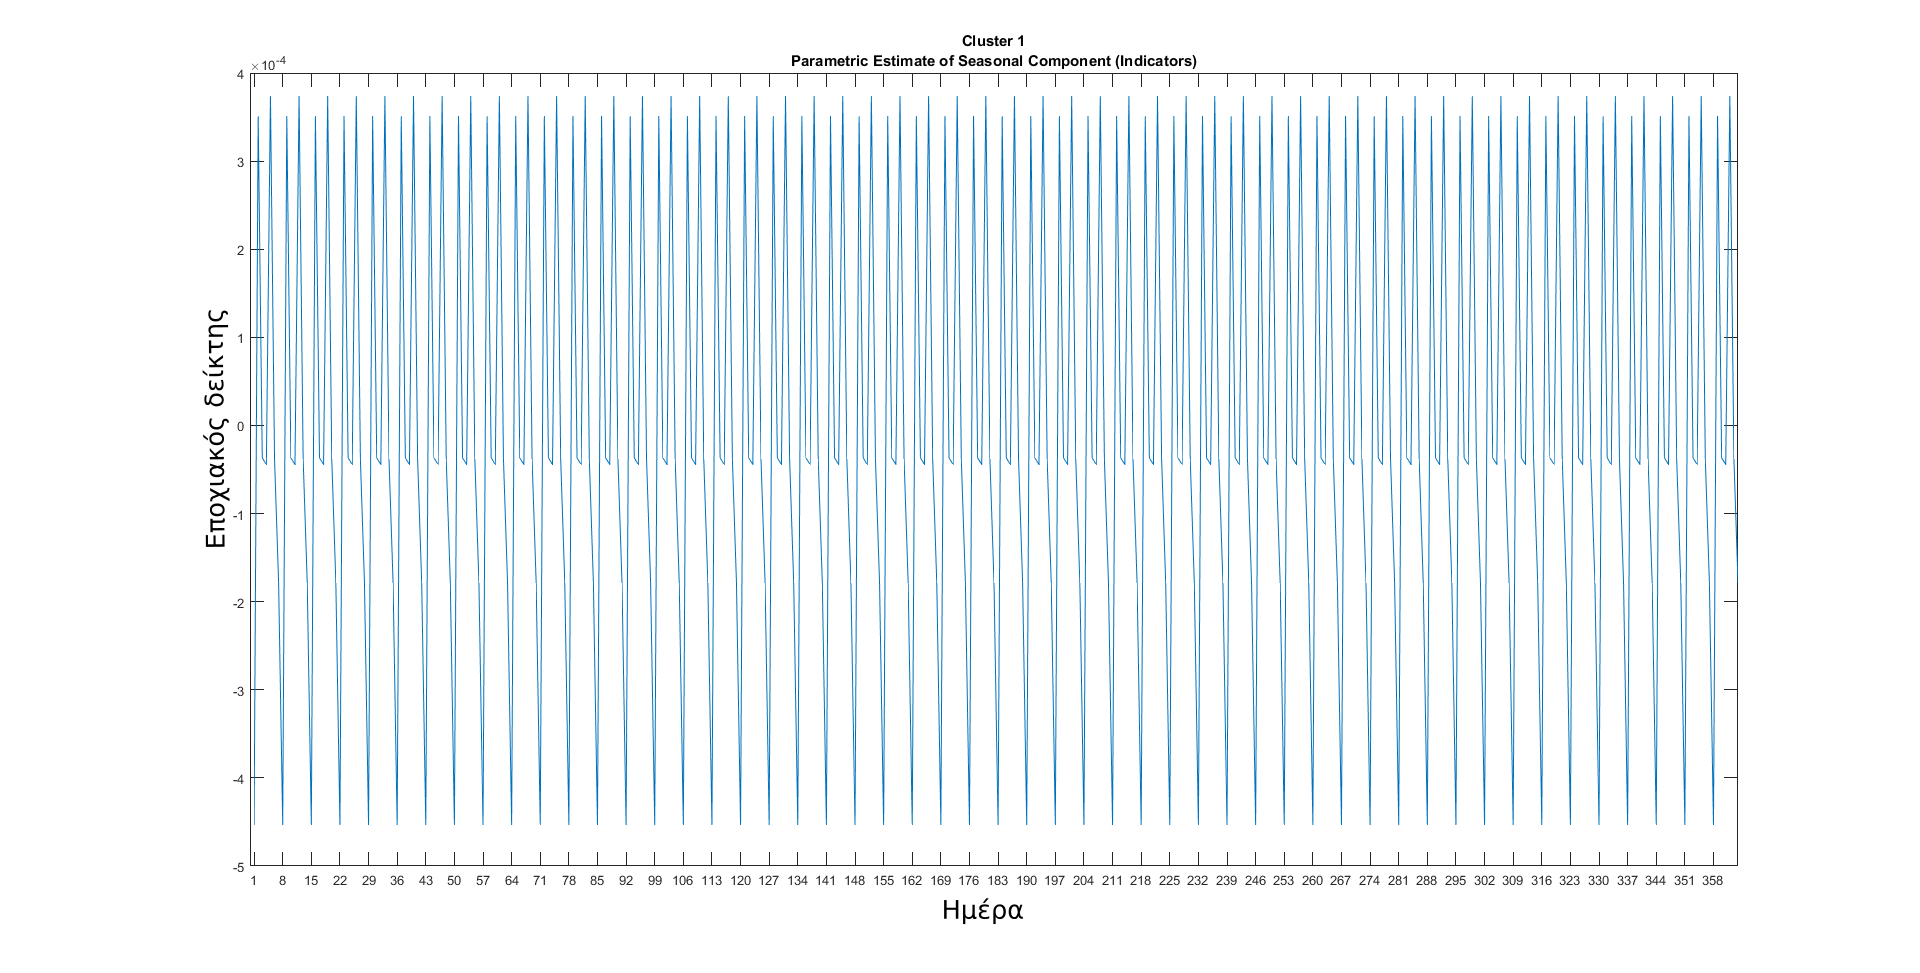
\includegraphics[width=180mm, height=100mm]{../../plots/Trend_estimation/seasonal_1.png}
\caption{Εβδομαδιαία εποχιακότητα ομάδας 1}
\label{fig:season 1}
\end{figure}
\begin{figure}[ht!]
\centering
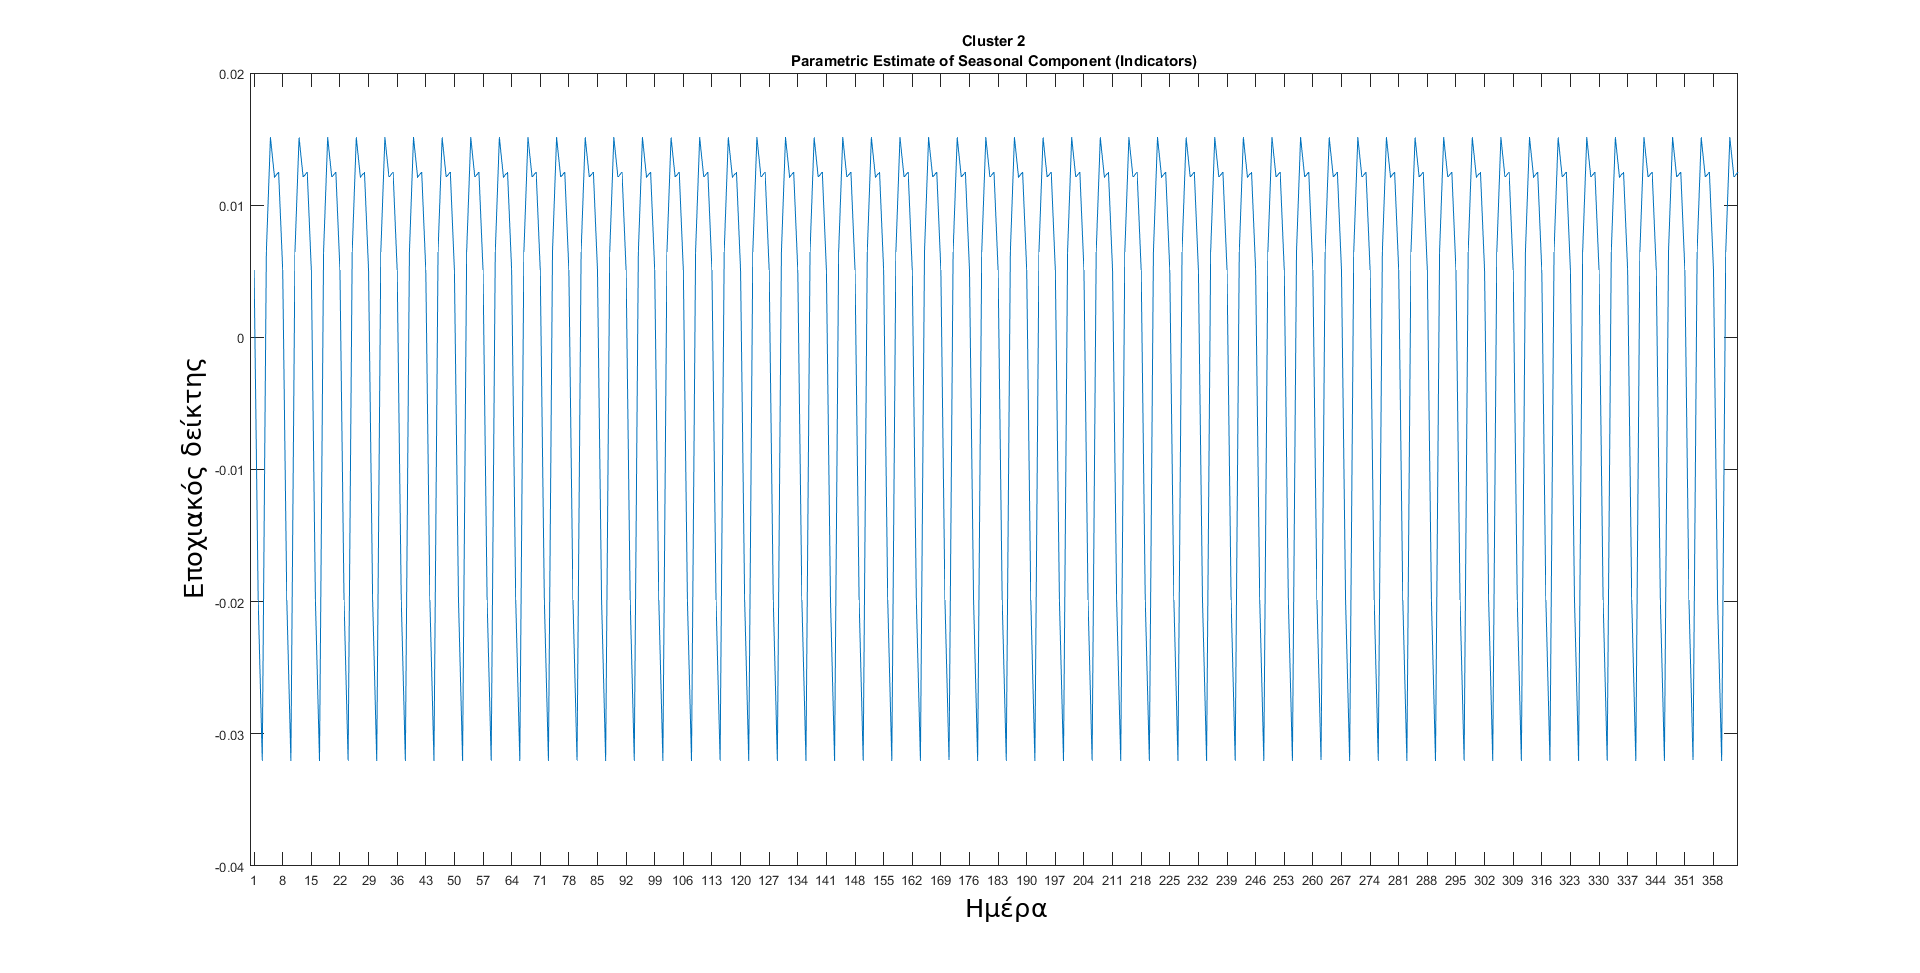
\includegraphics[width=180mm, height=100mm]{../../plots/Trend_estimation/seasonal_2.png}
\caption{Εβδομαδιαία εποχιακότητα ομάδας 2}
\label{fig:season 2}
\end{figure}
\begin{figure}[ht!]
\centering
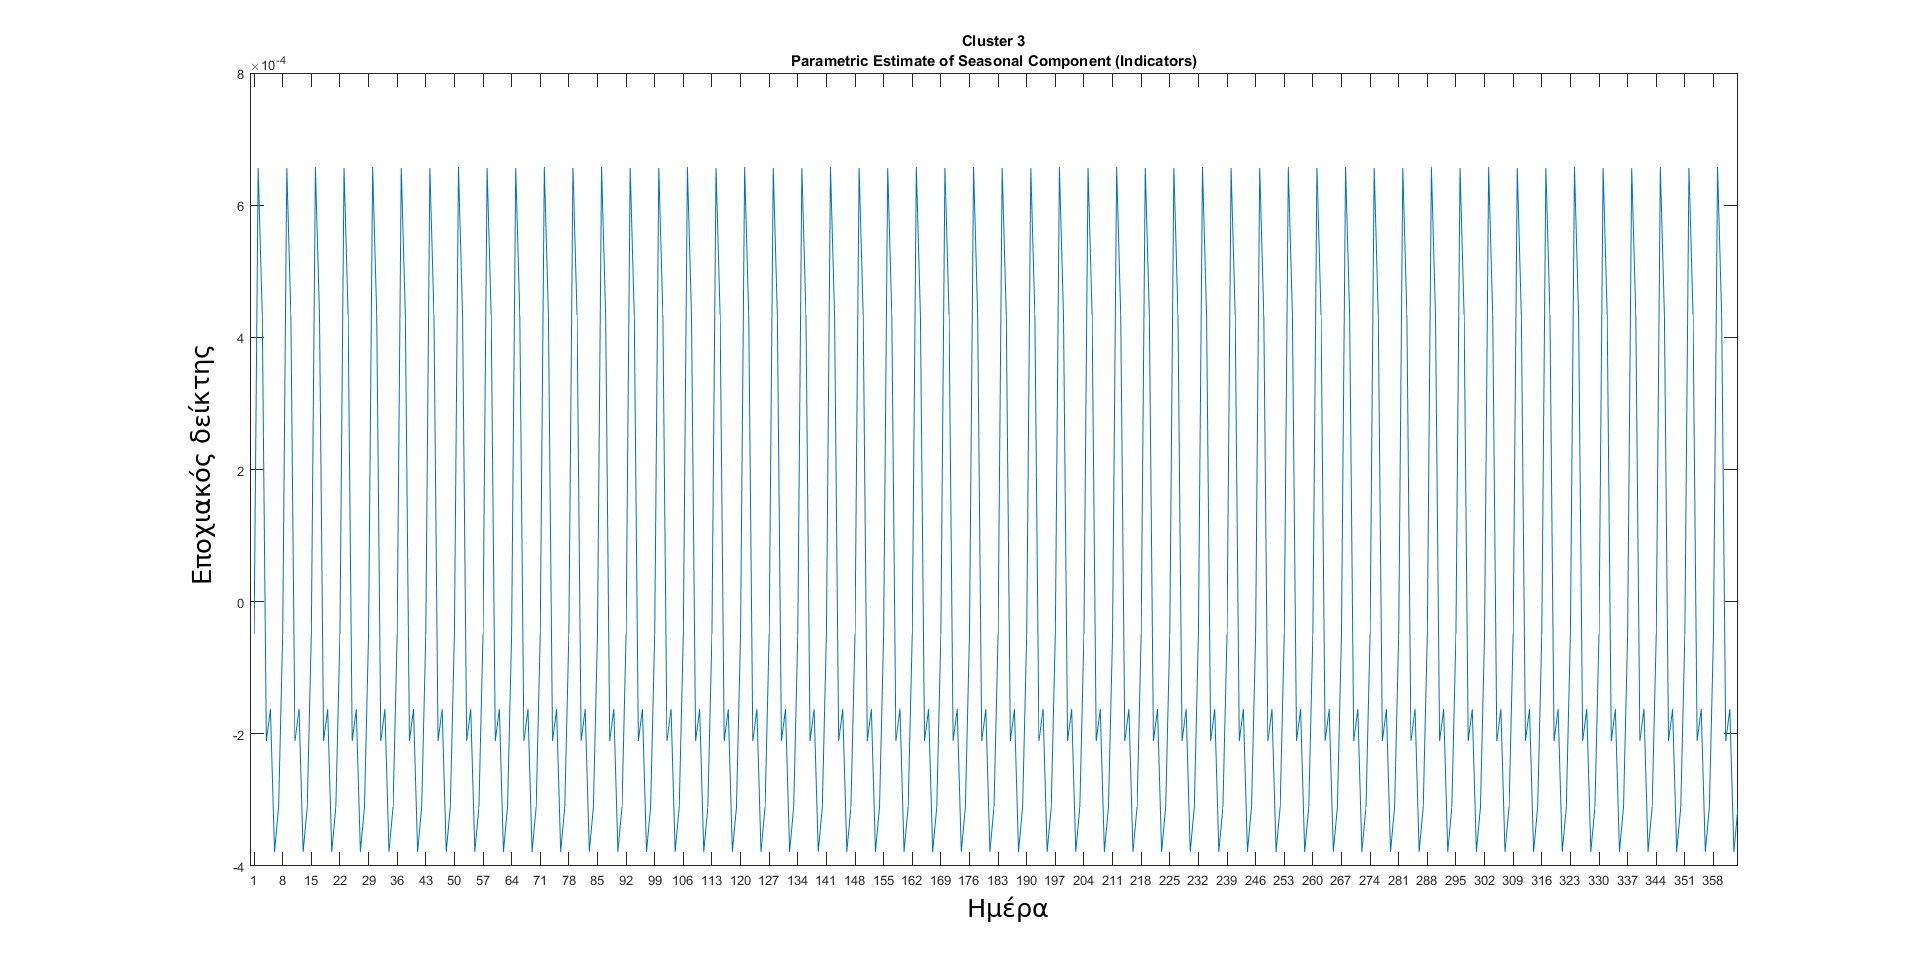
\includegraphics[width=180mm, height=100mm]{../../plots/Trend_estimation/seasonal_3.png}
\caption{Εβδομαδιαία εποχιακότητα ομάδας 3}
\label{fig:season 3}
\end{figure}
\begin{figure}[ht!]
\centering
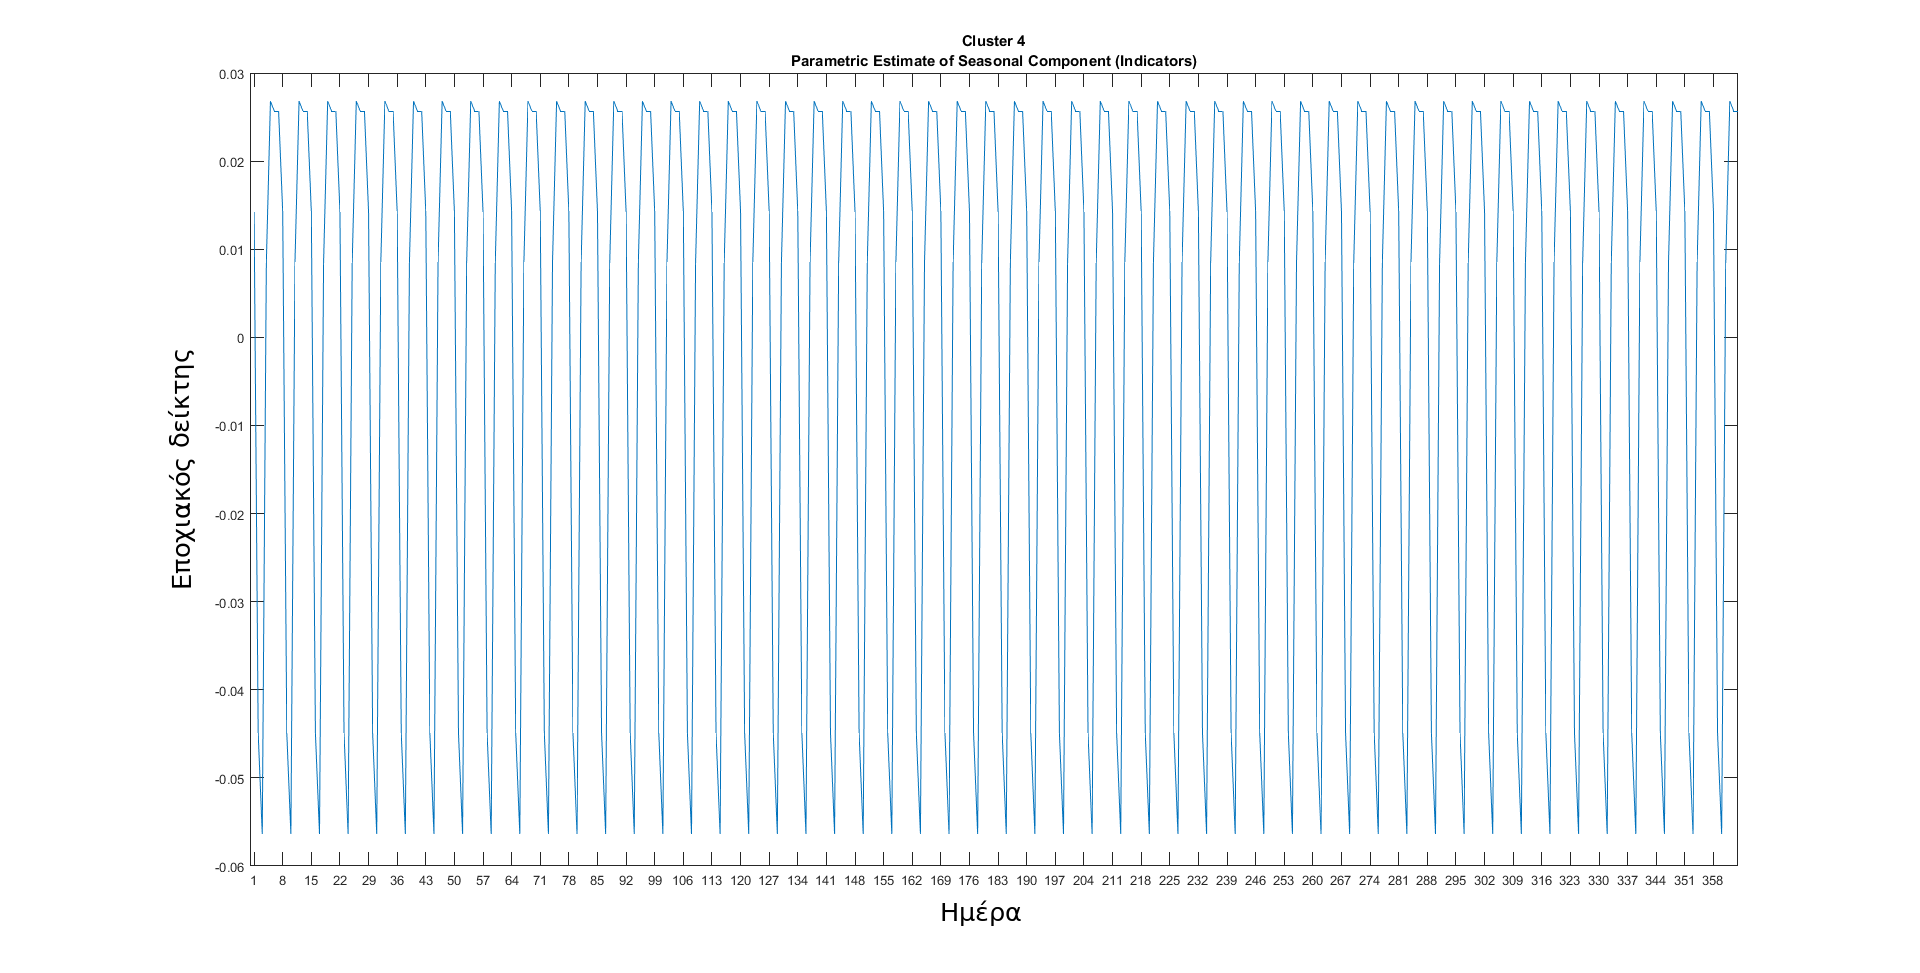
\includegraphics[width=180mm, height=100mm]{../../plots/Trend_estimation/seasonal_4.png}
\caption{Εβδομαδιαία εποχιακότητα ομάδας 4}
\label{fig:season 4}
\end{figure}
\subsubsection{Εκτίμηση σε διαστήματα ημέρας ανά μήνα}
Το διάστημα ενός μήνα αφήνει μεγαλύτερα περιθώριο εποπτείας της χρονοσειράς, ενώ ταυτόχρονα δημιουργεί αποτελέσματα με μεγαλύτερη συνοχή. Από την άλλη πλευρά οι 12 μήνες του έτους δεν μπορούν να εξάγουν πολύ ασφαλή δεδομένα αν συγκριθούν με τις 52 εβδομάδες.


Από την μηνιαία εποχιακότητα γίνεται εύκολα αντιληπτό πως ανάλογα με τον τύπο των καταναλωτών οι μέρες που έχουμε μέγιστη και ελάχιστη κατανάλωση διαφέρουν ριζικά. Ειδικότερα:
\begin{itemize}
\item Για τους καταναλωτές συστάδας 1 (επιχειρήσεις) έχουμε ελάχιστες καταναλώσεις στις 30 του μηνός.
\item Για τους καταναλωτές συστάδας 2 (οικιακοί καταναλωτές) έχουμε ελάχιστες καταναλώσεις στις 15 του μηνός.
\item Για τους καταναλωτές συστάδας 3 (οικιακοί καταναλωτές) έχουμε ελάχιστες καταναλώσεις στις 15 του μηνός.
\item Για τους καταναλωτές συστάδας 4 (επιχειρήσεις) έχουμε ελάχιστες καταναλώσεις στις 3 του μηνός.
\end{itemize}
\begin{figure}[ht!]
\centering
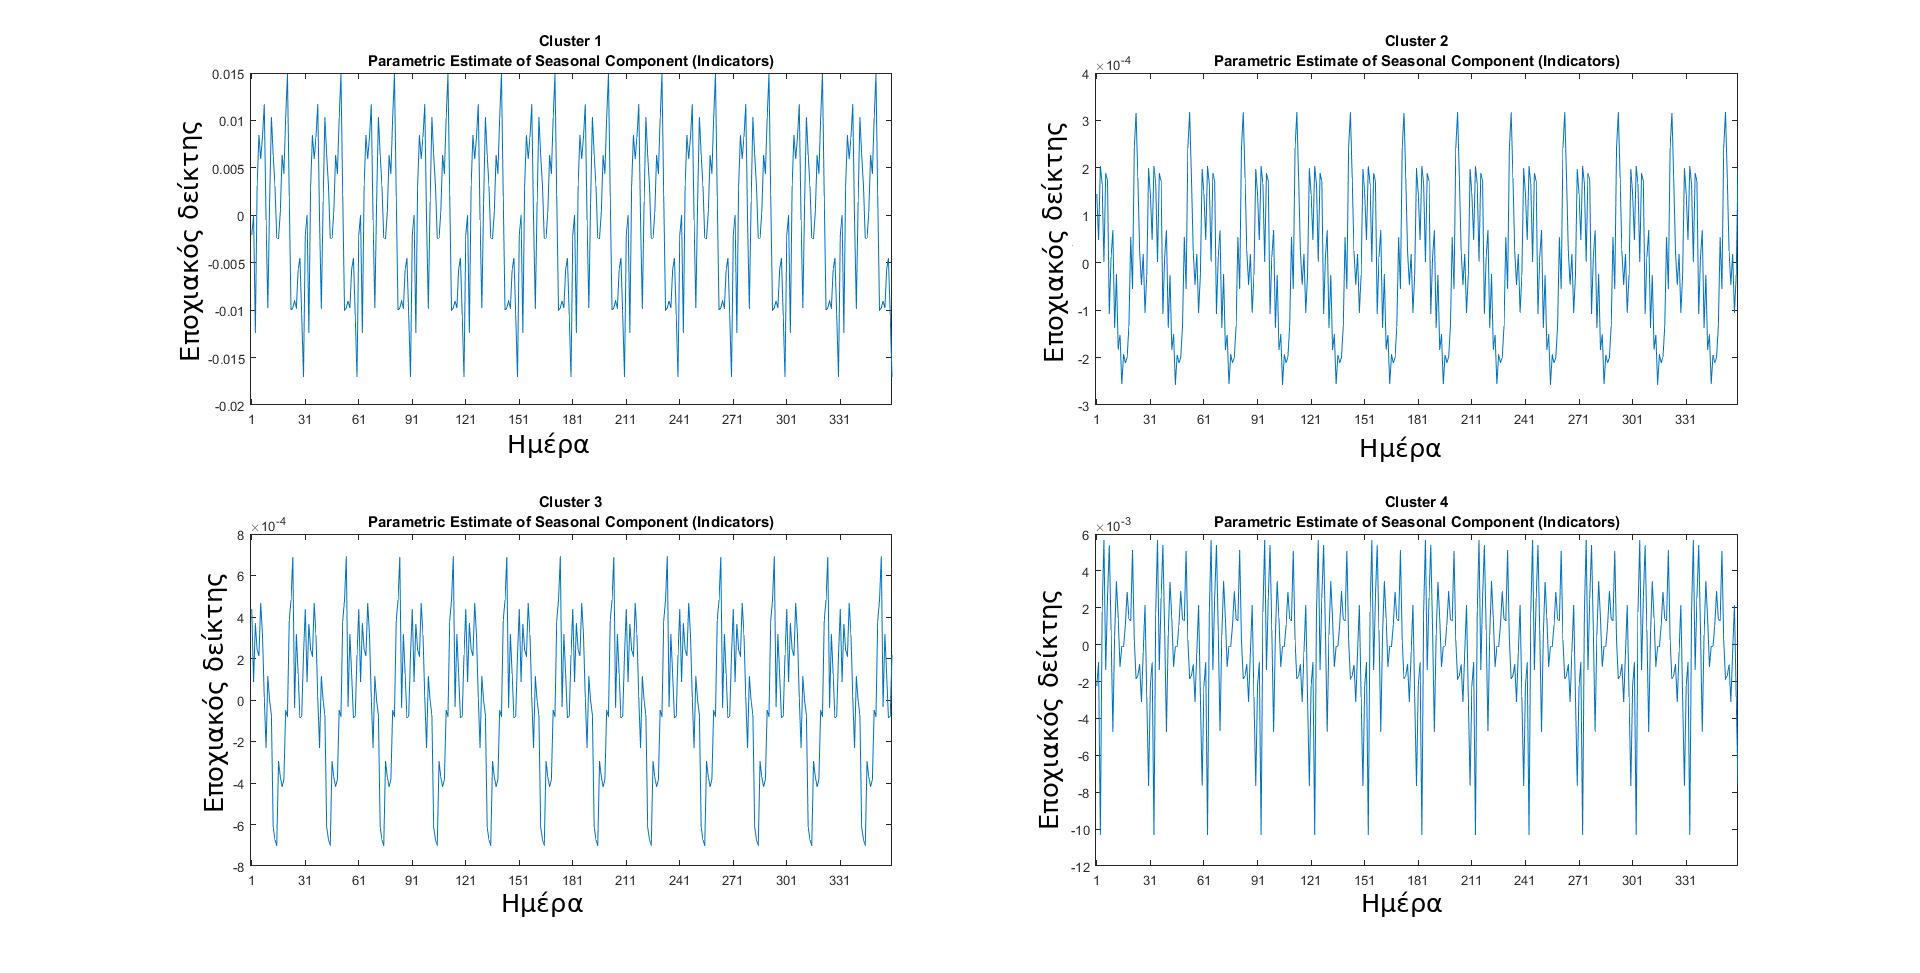
\includegraphics[width=180mm, height=120mm]{../../plots/Trend_estimation/seasonal_month_ALL.png}
\caption{Μηνιαία εποχιακότητα}
\label{fig:season daypermonth}
\end{figure}

\subsubsection{Αφαίρεση εποχιακών δεικτών}
Σε αυτό το σημείο είναι σημαντικό να παρατηρηθεί η κατανάλωση χωρίς τους εποχιακούς δείκτες. Με αυτό τον τρόπο καθίσταται ευκολότερη η θεώρηση της μορφής των κυματομορφών και η σύγκρισή τους με τις αρχικές καταναλώσεις του πρώτου μέρους. Αφαιρώντας τα εποχιακά χαρακτηριστικά οι καμπύλες πλησιάζουν περισσότερο στην παραβολική συνάρτηση. Έτσι η καταναλωτική τους τάση χωρίς τους εποχιακούς δείκτες γίνεται πιο έντονη και ευδιάκριτη.
\begin{figure}[ht!]
\centering
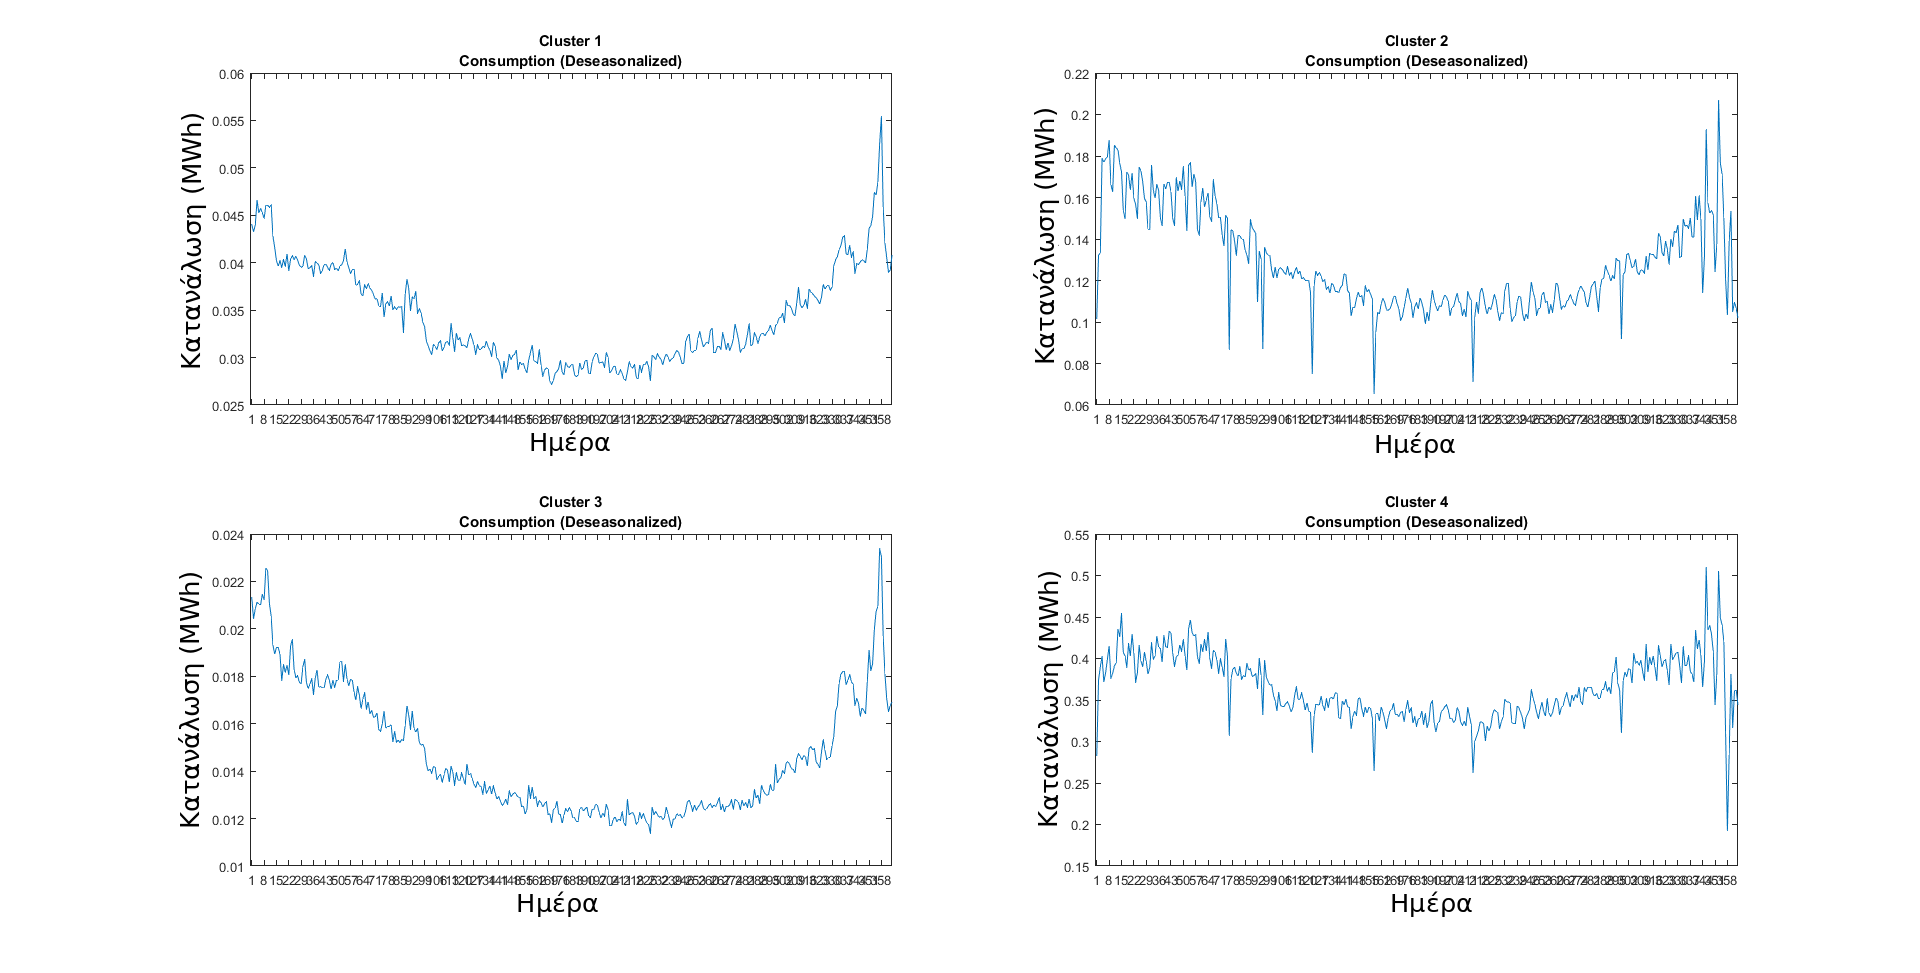
\includegraphics[width=180mm, height=120mm]{../../plots/Trend_estimation/Deseasonalized_ALL.png}
\caption{Κατανάλωση χωρίς εποχιακούς δείκτες ανά εβδομάδα}
\label{fig:deseason week}
\end{figure}
\newpage

\begin{figure}[ht!]
\centering
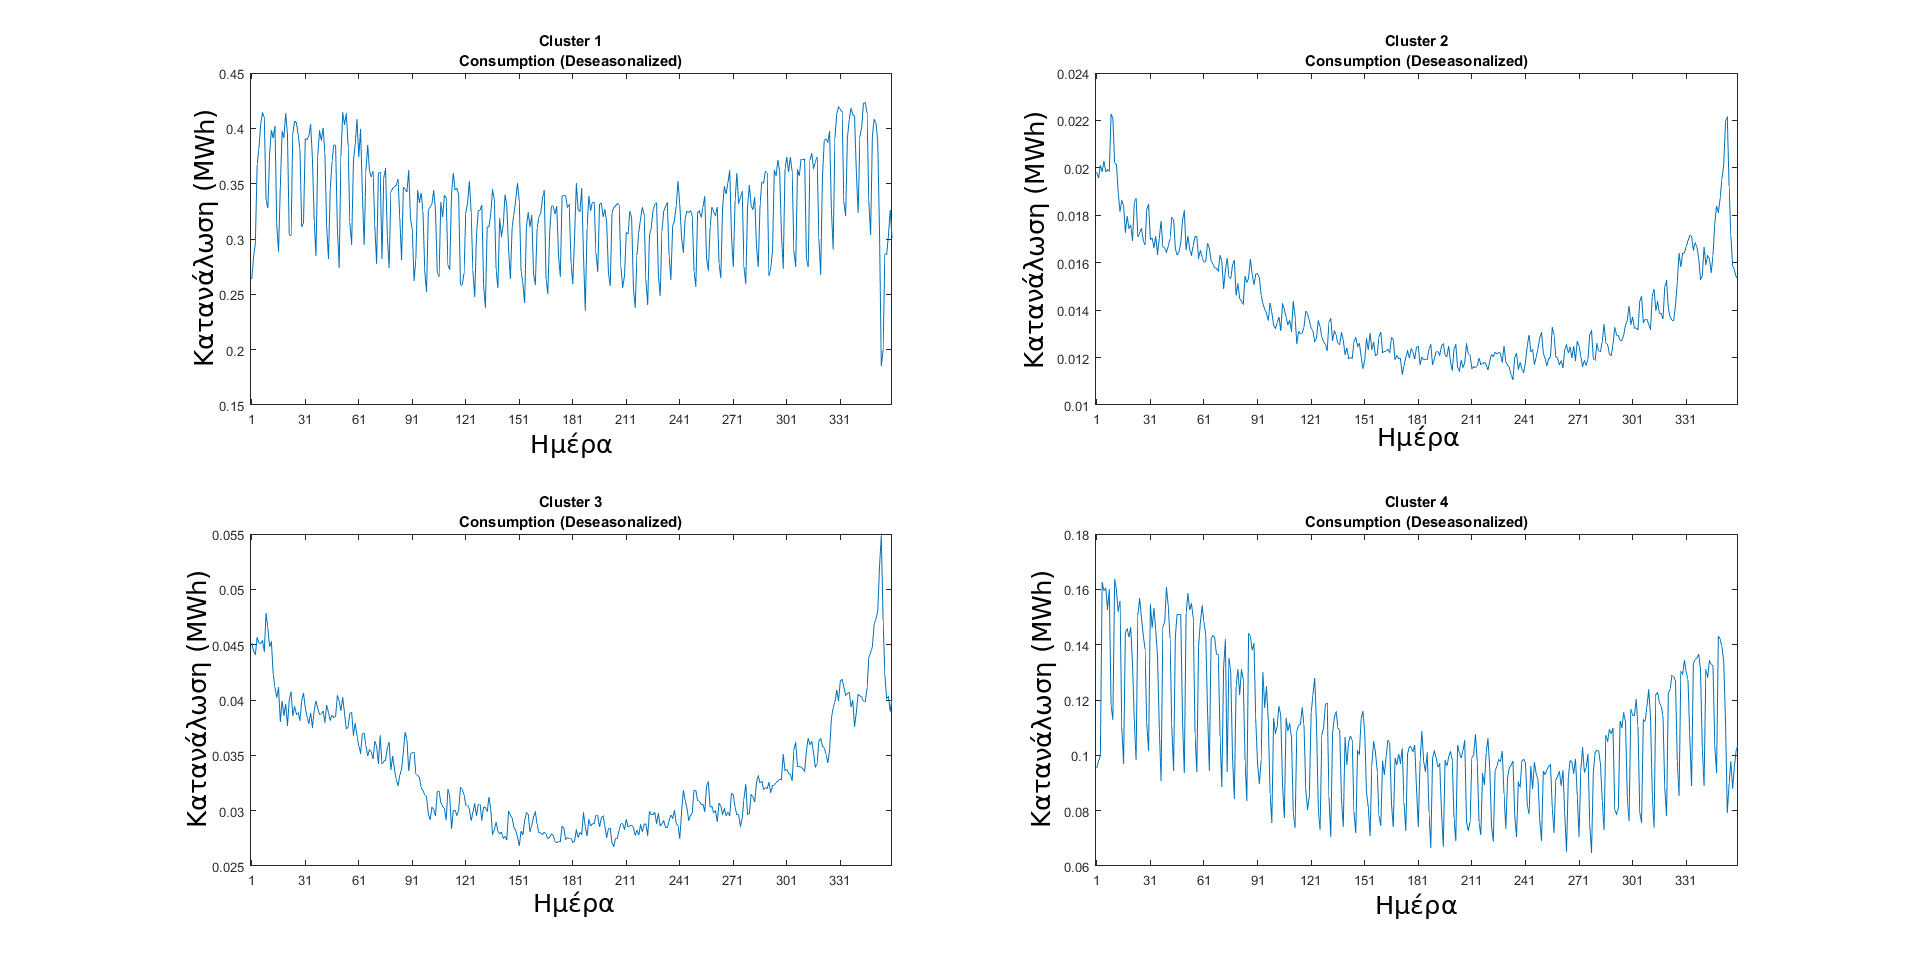
\includegraphics[width=180mm, height=120mm]{../../plots/Trend_estimation/Deseasonalized_month_ALL.png}
\caption{Κατανάλωση χωρίς εποχιακούς δείκτες ανά μήνα}
\label{fig:deseason month}
\end{figure}

\subsubsection{Εκτίμηση ακανόνιστης συνιστώσας}
Τέλος έχει ενδιαφέρουν να δούμε το βαθμό της τυχαιότητας που έχουμε στις καταναλώσεις των συστάδων που δημιουργήθηκαν. Αυτό επιτυγχάνεται αφαιρώντας την εποχιακή χρονοσειρά και την καταναλωτική τάση της αρχικής χρονοσειράς. Με αυτό τον τρόπο γίνεται σαφές ότι παρόλο την εποχιακότητα και την τάση οι χρονοσειρές έχουν αισθητό τυχαίο παράγοντα. Η αφαίρεση δημιουργεί αλλαγές στο επίπεδο της χεονοσειράς, σταθεροποιώντας έτσι το μέσο όρο της. Γίνεται αντιληπτό πως έχουν μη προβλέψιμα πρότυπα  τουλάχιστον με δεδομένα διάρκειας ενός έτους. Τέτοιου τύπου δεδομένα λέγενται στατικές χρονοσειρές.\cite{stationarity}
\begin{figure}[ht!]
\centering
\includegraphics[width=180mm, height=100mm]{../../plots/Trend_estimation/irregular_component_all.png}
\caption{Εκτίμηση ακανόνιστης συνιστώσας με εβδομαδιαία εποχιακότητα}
\label{fig:irregular week}
\end{figure}

\newpage
\begin{figure}[ht!]
\centering
\includegraphics[width=180mm, height=100mm]{../../plots/Trend_estimation/irregular_component_month_all.png}
\caption{Εκτίμηση ακανόνιστης συνιστώσας με μηνιαία εποχιακότητα}
\label{fig:irregular month}
\end{figure}
\subsubsection{Εξερεύνηση ημερών με χαμηλές καταναλώσεις}
Για να αντληθούν περαιτέρω χαρακτηριστικά των χρονοσειρών χρειάστηκε η υλοποίηση αλγορίθμου με διπλή συσταδοποίηση. Σύμφωνα με τον αλγόριθμο πρώτα συσταδοποιούνται οι καταναλωτές με βάση την ημερήσια κατανάλωση, εν συνεχεία για κάθε συστάδα δημιουργείται νέα ομαδοποίηση με βάση την ομοιότητα κάθε ημερήσιας κατανάλωσης. Με αυτό τον τρόπο μπορεί να παρατηρηθεί ποιες μέρες όμοιων καταναλωτών έχουν παρόμοιες καταναλώσεις. Καθίσταται έτσι εφικτό, να φιλτράρουμε από τα δεδομένα μας μέρες με χαμηλή κατανάλωση που γνωρίζουμε πως θα δυσκόλευαν το πρόβλημα της ταξινόμησης σε αληθή και αλλοιωμένα δεδομένα.

Τα αποτελέσματα του αλγορίθμου έδειξαν πως μόνο τα Σάββατα μιας συστάδας εμφανίζουν έντονη ομοιότητα οικιακών καταναλώσεων. Οι Κυριακές κατά κύριο λόγο συσταδοποιούνται με την υπόλοιπη εβδομάδα δημιουργώντας την εβδομαδιαία τάση, γεγονός που δείχνει πως για τους περισσότερους καταναλωτές η Κυριακή είναι εργάσιμη ημέρα. Παράλληλα, παρατηρείται πως ανά περιόδους οι καταναλώσεις δημιουργούν νέες συστάδες αφήνοντας μόνο τα Σάββατα να σπάνε την συνεχόμενη συσταδοποίηση. Στον Πίνακα \ref{tab:double clustering} φαίνεται πως ακόμη και στα Σάββατα δεν έχουμε απολύτως γεμάτες συστάδες.

\begin{table}[ht!]
\centering
\begin{tabular}{ |c||c|c|c|c|  }
 \hline
 \multicolumn{5}{|c|}{Συστάδες Καταναλωτών} \\
 \hline
 Συστάδες Σαββάτου  & Συστάδα 1& Συστάδα 2 &Συστάδα 3 &Συστάδα 4\\
 \hline
 Συστάδα 1 & 0  & 24 & 30 & 19\\
 Συστάδα 2 & 9  & 11 & 0  & 15\\
 Συστάδα 3 & 0  & 9  & 0  & 0\\
 Συστάδα 4 & 42 & 0  & 0  & 0\\
 Συστάδα 5 & 0  & 2  & 0  & 0\\
 Συστάδα 6 & 0  & 4  & 0  & 7\\
 Συστάδα 7 & 0  & 1  & 21 & 10\\
 \hline
\end{tabular}
\caption{Έλεγχος συσταδοποίησης Σαββάτου}
\label{tab:double clustering}
\end{table}

\subsubsection{Παρατηρήσεις}
Τα εμφανή χαρακτηριστικά εποχιακότητας και η εφαρμογή πολυωνύμου δευτέρου βαθμού στις χρονοσειρές θέτει καλό υποψήφιο τα μοντέλα πρόβλεψης χρονοσειρών. Με ένα τέτοιο σύστημα θα δημιουργείται μια πρόβλεψη κατανάλωσης από έμπιστους καταναλωτές για κάποιο χρονικό διάστημα. Εν συνεχεία θα αλλοιώνονται τα χαρακτηριστικά κάποιου μέρους των καταναλωτών και θα ελέγχεται αν ο αλγόριθμος μπορεί να διαχωρίσει τις αλλοιωμένες τιμές από αυτές που προέβλεψε.

\section{Προεπεξεργασία και καθάρισμα δεδομένων}
\section{Προσομοίωση απάτης}
\subsection{Τύποι απάτης}


\chapter{Αλγόριθμοι επιβλεπόμενης μάθησης}
Στο παρόν κεφάλαιο γίνεται μια εξερεύνηση στους αλγορίθμους επιβλεπόμενης μάθησης. Αυτό επιτεύχθηκε με τη χρήση γραμμικών και μη γραμμικών ταξινομητών, διερευνώντας διαφορετικά δεδομένα εισόδου για κάθε περίπτωση. Η βιβλιοθήκη που χρησιμοποιήθηκε για τη γραμμική ταξινόμηση ονομάζεται \en{LIBLINEAR} και χαρακτηρίζεται από εξαιρετικές επιδόσεις σε προβλήματα με μεγάλα σετ δεδομένων. Αντίστοιχα, για τη μη γραμμική ταξινόμηση χρησιμοποιήθηκε η βιβλιοθήκη \en{LIBSVM}, η οποία αναγάγει τα δεδομένα εισόδου σε μεγαλύτερο χώρο διαστάσεων.
\section{Θεωρία γραμμικής ταξινόμησης}
Η βιβλιοθήκη \en{LIBLINEAR} υποστηρίζει δύο δημοφιλείς δυαδικά γραμμικούς ταξινομητές: τη λογιστική παλινδρόμηση (\en{Logistic Regression}) και τη γραμμική μηχανή υποστήριξης διανυσμάτων (\en{linear SVM}). Δεδομένου ενός σετ εκπαίδευσης $(\mathbf{x}_i, y_i)$, $i=1,...,l$, όπου $\mathbf{x}_i\in\R^n$ είναι ένα χαρακτηριστικό διάνυσμα και $y_i=\pm1$ είναι οι ετικέτες, ένας γραμμικός ταξινομητής βρίσκει ένα διάνυσμα βαρών $\mathbf{w}\in\R^n$ επιλύοντας το ακόλουθο πρόβλημα:
\begin{center}
$min_{\mathbf{w}}f(\mathbf{w})\equiv\frac{1}{2}\mathbf{w}^T\mathbf{w}+C\sum_{i=1}^{l}\xi(y_i\mathbf{w}^T x_i)$
\end{center}
όπου $\mathbf{w}^T\mathbf{w}/2$ είναι ο όρος ομαλοποίησης, $\xi(y_i\mathbf{w}^T x_i)$ είναι η συνάρτηση κόστους (\en{loss function}) και $C>0$ είναι η παράμετρος ομαλοποίησης. Θεωρούμε τις συναρτήσεις κόστους στη λογιστική παλινδρόμηση (\en{LR}), στο  \en{L1-SVM}, στο \en{L2-SVM}:
\begin{center}
$\xi_{LR}(y\mathbf{w}^T\mathbf{x})=log(1 + exp(-y\mathbf{w}^T\mathbf{x}))$\\
$\xi_{L1}(y\mathbf{w}^T\mathbf{x})=(max(0, 1 - y\mathbf{w}^T\mathbf{x}))$\\
$\xi_{L2}(y\mathbf{w}^T\mathbf{x})=(max(0, 1 - y\mathbf{w}^T\mathbf{x}))^2$
\end{center}
Σε μερικές περιπτώσεις, η συνάρτηση διακρίσεως του ταξινομητή περιλαμβάνει και έναν παράγοντα βάρους $b$. Η \en{LIBLINEAR} χειρίζεται αυτόν τον παράγοντα αυξάνοντας το διάνυσμα $\mathbf{w}$ και κάθε παράδειγμα $\mathbf{x}_i$ με μία επιπλέον διάσταση: $\mathbf{w}^T \leftarrow [\mathbf{w}^T, b]$, $\mathbf{x}_i^T \leftarrow [\mathbf{x}_i^T, B]$, όπου B είναι μια σταθερά που ορίζεται από τον χρήστη. Η προσέγγιση για το \en{L1-SVM} και το  \en{L2-SVM} είναι μέσω της μεθόδου \en{coordinate descent}. Για το \en{LR} και το \en{L2-SVM}, η \en{LIBLINEAR} υλοποιεί μια μέθοδο περιοχής εμπιστοσύνης \en{Newton}. Στη φάση των δοκιμών, εκτιμάται ένα μέλος των δεδομένων $\mathbf{x}$ σαν θετικό εάν $\mathbf{w}^T\mathbf{x}>0$, και αρνητικό σε αντίθετη περίπτωση \cite{liblinearguide}, \cite{liblinearreport}.\par
Η μηχανή διανυσμάτων υποστήριξης εντάσσεται στο γενικότερο πλαίσιο της βελτιστοποίησης κυρτών συναρτήσεων και η προσέγγισή της έχει νόημα για όλους τους γραμμικούς ταξινομητές. Σε αδρές γραμμές, η διαδικασία εξελίσσεται σε τέσσερα κύρια βήματα:
\begin{enumerate}
\item Το πρόβλημα της εύρεσης του βελτίστου υπερεπιπέδου ξεκινά με μια δήλωση του προβλήματος στον πρωτεύοντα χώρο βαρών, ως ένα πρόβλημα βελτιστοποίησης με περιορισμούς.
\item Κατασκευάζεται η συνάρτηση \en{Lagrange} του προβλήματος.
\item Διατυπώνονται οι συνθήκες για τη βελτιστοποίηση της μηχανής.
\item Στήνεται το σκηνικό για την επίλυση του προβλήματος βελτιστοποίησης στο δυικό χώρο των πολλαπλασιαστών \en{Lagrange}.
\end{enumerate}
\par Όπως προαναφέρθηκε, το πρωτεύον πρόβλημα ασχολείται με μια κυρτή συνάρτηση κόστους και γραμμικούς περιορισμούς. Δοθέντος ενός τέτοιου προβλήματος βελτιστοποίησης με περιορισμούς, είναι δυνατό να κατασκευάσουμε ένα άλλο πρόβλημα, το αποκαλούμενο δυικό του πρωτεύοντος. Αυτό το δεύτερο πρόβλημα έχει την ίδια βέλτιστη τιμή με το πρωτεύον, αλλά με τους πολλαπλασιαστές \en{Lagrange} να παρέχουν τη βέλτιστη λύση \cite{haykin}.
\section{Εξερεύνηση γραμμικών ταξινομητών}
Αρχικά έγινε μια εξερεύνηση των μεθόδων που παρέχει η \en{LIBLINEAR} για την επίλυση του προβλήματος. Λαμβάνοντας υπόψη 2.000 καταναλώσεις πελατών με ωριαίες μετρήσεις, επιλέχθηκε 10\% ποσοστό ρευματοκλοπών για την προσομοίωση. Η βιβλιοθήκη που χρησιμοποιήθηκε περιλαμβάνει 7 διαφορετικούς συνδυασμούς ταξινομητών και συναρτήσεων κόστους, για να μπορούν να αντιμετωπιστούν όσο το δυνατόν περισσότερα προβλήματα. Παρ' όλα, αυτά οι μέθοδοι \en{L1} είναι παλαιότερες εκδόσεις των \en{L2} και αναμένεται να έχουν χειρότερα αποτελέσματα στις δοκιμές. Για την σφαιρική αντιμετώπιση του προβλήματος χρησιμοποιήθηκαν όλοι οι ταξινομητές που παρέχονται από τη βιβλιοθήκη σε κάθε τύπο απάτης. Παρακάτω παρατίθενται οι συνδυασμοί ταξινομητών και συναρτήσεων κόστους που δοκιμάστηκαν και τα αποτελέσματα σε κάθε τύπο απάτης.\par
\begin{enumerate}
\item \en{L2} ομαλοποιημένη λογιστική παλινδρόμηση (πρωτεύον)
\item \en{L2} oμαλοποιημένος ταξινομητής με \en{L2} συνάρτηση κόστους διανυσμάτων υποστήριξης (δυικό)
\item \en{L2} oμαλοποιημένος ταξινομητής με \en{L2} συνάρτηση κόστους διανυσμάτων υποστήριξης (πρωτεύον)
\item \en{L2} oμαλοποιημένη ταξινομητής με \en{L1} συνάρτηση κόστους διανυσμάτων υποστήριξης (δυικό)
\item Ταξινόμηση διανυσμάτων υποστήριξης από \en{Crammer} και \en{Singer}
\item \en{L1} oμαλοποιημένος ταξινομητής με \en{L2} συνάρτηση κόστους διανυσμάτων υποστήριξης
\item \en{L1} ομαλοποιημένη λογιστική παλινδρόμηση
\item \en{L2} ομαλοποιημένη λογιστική παλινδρόμηση (δυικό)
\end{enumerate}
\par Αρχικά έγινε μια δοκιμή σε 2.000 καταναλωτές με το 10\% τους να έχει εισροή μη τεχνικών απωλειών. Τα διανύσματα των καταναλωτών είχαν 8.760 χαρακτηριστικά που αντιστοιχούν στις ώρες ενός έτους. Για να ευρεθεί η συνολική απόδοση όλων των γραμμικών ταξινομητών, έγιναν δοκιμές και στους τέσσερις τύπους απάτης (1, 2, 3, μικτός) και για αυτό και τα αποτελέσματα αναμένονται σχετικά χαμηλά. Ειδικότερα θα εξαχθεί ο μέσος όρος του \en{F1 score} και του \en{Accuracy} από τη δοκιμή κάθε αλγορίθμου και στους τέσσερις τύπους απάτης.\par
Χρησιμοποιώντας 70\% του δείγματος για τις εκπαιδεύσεις κάθε ταξινομητή και 30\% για τις προβλέψεις, πραγματοποιήθηκαν τέσσερις δοκιμές σε κάθε ένα από τους οκτώ συνολικά αλγορίθμους. Τα αποτελέσματα φαίνονται παρακάτω στον Πίνακα \ref{tab:meanlinearmetrics}.
\begin{table}[ht!]
\centering
\begin{tabular}{ |c||c|c|c|c|c|c|c|c|  }
 \hline
 Αλγόριθμος & 1 & 2 & 3 & 4 & 5 & 6 & 7& 8 \\
 \hline
 \en{F1 score} & 23.92 & 31.99 & 30.19 &  28.67& 32.66 & 29.28 & 20.43 &24.04\\
 \hline
\en{Accuracy} & 91.36 & 90.41 & 90.46 &  90.56 & 90.15 & 90.37 & 91.43 & 91.35\\
\hline
\hline
  Μέσος όρος & 57.64 & 61.2 & 60.33 & 59.61 & 61.4 & 59,83 & 55.93 & 57.7\\
\hline
\end{tabular}
\caption{Μέσοι όροι μετρικών στις δυσκολότερες απάτες}
\label{tab:meanlinearmetrics}
\end{table}
\par Εύκολα παρατηρείται από τον Πίνακα \ref{tab:meanlinearmetrics} πως η επίδοση των αλγορίθμων στο \en{F1 score} είναι περιορισμένη, υποδηλώνοντας δυσκολία στην ταξινόμηση. Αυτό οφείλεται στις κακές επιδόσεις των αλγορίθμων στις απάτες τύπου δύο, τρία και μικτού. Από την άλλη πλευρά τα αποτελέσματα του \en{Accuracy} είναι υποσχόμενα, αλλά πρέπει να ληφθεί υπόψη πως λόγω του χαμηλού ποσοστού κλοπών ένας κακός αλγόριθμος θα μπορούσε να προβλέπει πάντα αρνητικά και να είχε 90\% \en{Accuracy}. Καθίσταται, λοιπόν, σαφές πως οι ταξινομητές έχουν μεγάλη δυσκολία να διαχωρίσουν τις προσομοιώσεις μη τεχικών απωλειών με μεγάλο τυχαίο παράγοντα από τις φυσιολογικές καταναλώσεις. Παρ' όλα αυτά, τα αποτελέσματα των δοκιμών στις απάτες τύπου 1 είναι ικανοποιητικά και δημιουργούν ανάγκη περαιτέρω ανάλυσης.\par
Η διαφορά της απόδοσης των γραμμικών ταξινομητών σε κάθε είδος απάτης και ειδικότερα σε σχέση με της κλοπές τύπου 1 υπήρξε ο λόγος εκκίνησης νέου κύκλου δοκιμών. Έγινε λοιπόν δοκιμή κάθε αλγορίθμου σε απάτες τύπου 1 με 10\% ποσοστό ρευματοκλοπών. Το 70\% των δεδομένων χρησιμοποιήθηκε για τις εκπαιδεύσεις των ταξινομητών και το υπόλοιπο 30\% για τις προβλέψεις των αλγορίθμων.
\begin{table}[ht!]
\centering
\begin{tabular}{ |c||c|c|c|c|c|  }
 \hline
 Αλγόριθμος & \en{DR}  & \en{FPR} & \en{Accuracy} & \en{F1 score} & \en{BDR \%} \\
 \hline
1 & 77.44 & 1.56 & 96.37 & 80.78 & 85 \\
  \hline
2 & 79.70 & 1.81 & 96.37 & 81.23 & 83 \\
  \hline
3 &78.95 & 2.22 & 95.93 & 79.25 & 80 \\
  \hline
4 & 78.95 & 2.05 & 96.07 & 79.85 & 81\\
  \hline
5 & 78.20 & 1.81 & 96.22 & 80.31 & 83\\
 \hline
6 & 77.44 & 2.14 & 95.85 & 78.63 & 80 \\
 \hline
7 & 75.94 & 1.81 & 96.00 & 78.91 & 82\\
 \hline
8 & 79.70 & 1.81 & 96.37 & 81.23 & 83\\
 \hline
\end{tabular}
\caption{Αποτελέσματα δοκιμής τύπου 1 χωρίς κανονικοποίηση}
\label{tab:exploreclassifiers1nonorm}
\end{table}

\subsection{Παρατηρήσεις}
Παρατηρώντας τους πίνακες αποτελεσμάτων εύκολα αποδεικνύεται η αρχική υπόθεση πως οι ταξινομητές και συναρτήσεις κόστους \en{L2} έχουν καλύτερη συμπεριφορά ως προς την αντιμετώπιση του προβλήματος αναγνώρισης χρονοσειρών.  Πιο συγκεκριμένα, για την τελική επιλογή του συνδυασμού μεθόδων επιλέχθηκαν δύο μετρικές για να καθορίσουν την επιλογή του καλύτερου πακέτου. Λήφθηκε υπόψη η μεταβολή της ευστοχίας (\en{Accuracy}) και παράχθηκε μέσος όρος για όλους τους τύπους. Παράλληλα, υπολογίστηκε μέσος όρος των δοκιμών με γνώμονα το καλύτερο \en{F1 score}, καθώς είναι μια αρκετά ζυγισμένη μετρική για τα προβλήματα ταξινόμησης. Βάσει, λοιπόν, του Πίνακα \ref{tab:meanlinearmetrics} την καλύτερη επίδοση έχει το πρωτεύον πρόβλημα που αποτελείται από \en{L2} oμαλοποιημένο ταξινομητή με \en{L2} συνάρτηση κόστους διανυσμάτων υποστήριξης, καθώς όπως μπορεί και να φανεί στον Πίνακα \ref{tab:accuracytypes} του Παραρτήματος, η μηχανή διανυσμάτων υποστήριξης \en{Crammer} και \en{Singer} έχει καλύτερη επίδοση στους τύπους 2, 3 και στον μικτό. Αλλά, στην παρούσα φάση θα ασχοληθούμε με την απάτη τύπου 1.
\section{Εξερεύνηση διαφορετικών τρόπων κανονικοποίησης}
Το σκέλος της κανονικοποίησης των δεδομένων είναι ζωτικής σημασίας για κάθε σύστημα μηχανικής μάθησης. Η κανονικοποίηση των δεδομένων υλοποιείται, μειώνοντας το εύρος των τιμών σε οποιαδήποτε σχετικά μικρό εύρος. Συνηθέστερη πετυχημένη πρακτική είναι η αναγωγή των τιμών σε εύρος [0,1] ή [-1,1] με στόχο τη βελτίωση της επίδοσης και της ταχύτητας του αλγορίθμου.\par
Επιλέγοντας λοιπόν το σύνηθες δείγμα 2.000 καταναλωτών με ωριαίες μετρήσεις έτους και 10\% ποσοστό καταναλωτών με μη τεχνικές απώλειες, οι αλγόριθμοι εκπαιδεύτηκαν με 70\% του δείγματος και η πρόβλεψη επιτεύχθηκε με 30\% για κάθε μέθοδο κανονικοποίησης.\par
Η βελτίωση της επίδοσης του αλγορίθμου επιτυγχάνεται σε μεγάλο βαθμό στη συγκεκριμένη περίπτωση από την κανονικοποίηση στο εύρος [0,1], βελτιώνοντας σε μικρό βαθμό τις μετρικές και μειώνοντας σχεδόν 10 φορές τον χρόνο εκτέλεσης της εκπαίδευσης. Στον Πίνακα \ref{tab:explorenormalization} παρατίθενται τα αποτελέσματα των βέλτιστων ταξινομητών σε κάθε είδος κανονικοποίησης.\par

\begin{table}[ht!]
\centering
\begin{tabular}{ |c|c|c|c|c|c|c|c|  }
 \hline
 Κανονικοποίηση & \en{DR}  & \en{FPR} & \en{Accuracy} & \en{F1 score} & \en{BDR \%}& χρόνος εκπαίδευσης \en{(s)} \\
 \hline
 [0,1] & 80.87 & 1.54 & 96.96 & 81.94 & 85 & 6.492741\\
  \hline
 [-1,1]& 91.67 & 21.23 & 80.15 & 49.62 & 32 & 551.264250\\
  \hline
 - &79.70 & 1.81 & 96.37 & 81.23 & 83 & 58.246916 \\
  \hline
\end{tabular}
\caption{Αποτελέσματα κανονικοποιήσεων}
\label{tab:explorenormalization}
\end{table}

\section{Εξερεύνηση χρονικής υποδιαίρεσης χρονοσειρών}
Ολοκληρώνοντας την εξερεύνηση των ταξινομητών, απαιτείται να γίνει έλεγχος στις χρονικές υποδιαιρέσεις των χρονοσειρών. Για αυτό το σκοπό έγινε δοκιμή του πιο εύστοχου ταξινομητή σε 2.000 καταναλωτές με ποσοστό ρευματοκλοπών 10\% και μόνο απάτες τύπου 1. Στη δοκιμή οι χρονοσειρές διαιρέθηκαν σε ημερήσιες, ωριαίες και ημίωρες μετρήσεις, λαμβάνοντας υπόψη όχι μόνο τις μετρικές ευστοχίας, αλλά και τον χρόνο εκτέλεσης της εκπαίδευσης κάθε ταξινομητή. Επιλέγοντας ως συνήθως 70\% των δεδομένων για εκπαίδευση και το υπόλοιπο για πρόβλεψη, έγιναν δοκιμές για κάθε χρονική υποδιαίρεση.\par
Στον Πίνακα \ref{tab:timedivision} εμφανίζεται, όπως αναμενόταν πως όσο αυξάνεται η συχνότητα των μετρήσεων τόσο πιο εύστοχος γίνεται ο ταξινομητής. Ωστόσο, ο χρόνος εκτέλεσης της εκπαίδευσης φαίνεται να επηρεάζεται έντονα από διαφορετικές χρονικές υποδιαιρέσεις με την ταξινόμηση με συχνότητα λήξης ανά ημέρα να είναι σημαντικά γρηγορότερη από τις υπόλοιπες, αλλά παρουσιάζεται σχετική δυσκολία στην αναγνώριση της απάτης. 

\begin{table}[ht!]
\centering
\begin{tabular}{ |c||c|c|c|c|c|c|  }
 \hline
 Συχνότητα & \en{DR}  & \en{FPR} & \en{Accuracy} & \en{F1 score} & \en{BDR \%} & χρόνος εκπαίδευσης \en{(s)}\\
 \hline
μέρες & 81.62 & 2.55 & 95.85 & 79.86 & 78 & 0.069182\\
 \hline
ώρες & 82.88 & 2.16 & 96.22 & 82.59 & 81 & 4.152410\\
  \hline
ημίωρα & 81.08 & 1.66 & 96.44 & 83.33 & 84 & 12.169304\\
  \hline
\end{tabular}
\caption{Αποτελέσματα δοκιμής χρονικής υποδιαίρεσης}
\label{tab:timedivision}
\end{table}

\section{Θεωρία Μηχανών Διανυσμάτων Υποστήριξης}
Για την ταξινόμηση με μηχανές διανυσμάτων υποστήριξης επιλέχθηκε η βιβλιοθήκη \en{LIBSVM}, η οποία προέρχεται από τους ίδιους δημιουργούς της \en{LIBLINEAR}. Σκοπός του \en{SVM} είναι η παραγωγή μοντέλων (βάσει των δεδομένων εκπαίδευσης), τα οποία προβλέπουν τα χαρακτηριστικά των δεδομένων δοκιμής βάσει μόνο των πληροφοριών που αντλούνται από τις τιμές των δεδομένων.\par
Ξεκινώντας από τα δεδομένα εκπαίδευσης έχουμε ζευγάρια παραδειγμάτων-δυαδικών χαρακτηριστικών $(\mathbf{x}_i,y_i)$,$i=1,...,l$ όπου $\mathbf{x}_i\in\R^n$ και $y\in\{1,-1\}^l$, ενώ οι μηχανές διανυσμάτων υποστήριξης \en{(SVM)} απαιτούν την λύση του παρακάτω προβλήματος βελτιστοποίησης:
\begin{center}
$min_{\mathbf{w},\mathbf{b},\mathbf{\xi}} \frac{1}{2}\mathbf{w}^T\mathbf{w}+C\sum_{i=1}^l\xi_i$\\
δεδομένου $y_i(\mathbf{w}^T\phi(\mathbf{x}_i)+b)\geq 1-\xi_i$,\\
$\xi_i \geq 0$
\end{center}
\par Εδώ τα διανύσματα εκπαίδευσης $\mathbf{x}_i$ ανάγονται σε μεγαλύτερο (ίσως άπειρο) χώρο διαστάσεων από τη συνάρτηση $\phi$. Τα \en{SVM} βρίσκουν ένα γραμμικά διαχωρίσιμο υπερεπίπεδο με μέγιστο περιθώριο σε αυτό χώρο ανώτερων διαστάσεων. $C>0$ είναι ο παράγοντας που θέτει ποινή στον παράγοντα λάθους (\en{error term}). Επιπροσθέτως, η σχέση $K(\mathbf{x}_i,\mathbf{x}_j)\equiv \phi(\mathbf{x}_i)^T\phi(\mathbf{x}_j)$ ονομάζεται συνάρτηση πυρήνα. Παρόλο που νέοι πυρήνες προτείνονται από ερευνητές, έχουν θεσπιστεί οι ακόλουθοι:
\begin{itemize}
\item Γραμμικός: $K(\mathbf{x}_i,\mathbf{x}_j)= \mathbf{x}_i^T\mathbf{x}_j$.
\item Πολυωνυμικός: $K(\mathbf{x}_i,\mathbf{x}_j)= (\gamma\mathbf{x}_i^T\mathbf{x}_j+r)^d$, $\gamma=\frac{1}{2\sigma^2}>0$.
\item \en{RBF}: $K(\mathbf{x}_i,\mathbf{x}_j)= exp(-\gamma\|\mathbf{x}_i-\mathbf{x}_j\|^2)$, $\gamma>0$.
\item Σιγμοειδής: $K(\mathbf{x}_i,\mathbf{x}_j)= tanh(\gamma\mathbf{x}_i^T\mathbf{x}_j +r)$.
\end{itemize}
Εδώ τα $\gamma$, $r$ και $d$ είναι παράμετροι των πυρήνων \cite{libsvmguide}.\par
Χρησιμοποιώντας τη μέθοδο των πολλαπλασιαστών \en{Lagrange} μπορεί να διατυπωθεί το δυικό πρόβλημα για τα μη διαχωρίσιμα πρότυπα. Δοθέντος του δείγματος εκπαίδευσης $\{(\mathbf{x}_i,y_i)\}_{i=1}^N$, βρίσκονται οι πολλαπλασιαστές \en{Lagrange} $\{\alpha\}_{i=1}^N$ που μεγιστοποιούν την αντικειμενική συνάρτηση:\\
\begin{center}
$Q(\alpha)=\sum_{i=1}^N\alpha_i-\frac{1}{2}\sum_{i=1}^N\sum_{j=1}^N\alpha_i\alpha_jy_iy_j\mathbf{x}_i^T\mathbf{x}_j$
υπό τους περιορισμούς
$\sum_{i=1}^N\alpha_i d_i=0$\\
$0 \leq \alpha_i \leq C$ για $i=1,2, ...,N$\\
\end{center}
όπου $C$ είναι μια καθοριζόμενη από το χρήστη θετική παράμετρος \cite{haykin}.
\subsection{Θεωρία επιλογής πυρήνα \en{RBF}}
Γενικώς, ο πυρήνας δικτύου ακτινικής συνάρτησης βάσης (\en{RBF}) είναι μια λογική πρώτη επιλογή. Αυτός ο πυρήνας ανάγει μη γραμμικά τα δείγματα σε υψηλότερο χώρο διαστάσεων που μπορεί να διαχειριστεί την περίπτωση κατά την οποία η σχέση μεταξύ της τάξης και της τιμής είναι μη γραμμική. Επιπροσθέτως, ο γραμμικός πυρήνας είναι μια ειδική περίπτωση του \en{RBF}, καθώς ο γραμμικός πυρήνας με την παράμετρο ποινής $\check{C}$ έχει την ίδια επίδοση με τον \en{RBF} με δύο παραμέτρους ($C$,$\gamma$). Ακόμη, ο πυρήνας με σιγμοειδή συνάρτηση συμπεριφέρεται όπως με \en{RBF} για συγκεκριμένες παραμέτρους.\par
Ο δεύτερος λόγος είναι ο αριθμός των υπερπαραμέτρων, οι οποίες επηρεάζουν την πολυπλοκότητα της επιλογής μοντέλου. Ο πολυωνυμικός πυρήνας έχει περισσότερες υπερπαραμέτρους από τον \en{RBF} πυρήνα.\par
Τέλος, ο πυρήνας \en{RBF} έχει λιγότερες αριθμητικές δυσκολίες. Το χαρακτηριστικό κλειδί είναι πως το $0<K_{ij}\leq1$ είναι σταθερά του πολυωνυμικού πυρήνα του οποίου οι τιμές μπορούν να φτάνουν το άπειρο $(\gamma\mathbf{x}_i^T\mathbf{x}_j+r>1)$ ή το μηδέν $(\gamma\mathbf{x}_i^T\mathbf{x}_j+r<1)$ ενώ ο βαθμός είναι ήδη μεγάλος. Επίσης, πρέπει να σημειωθεί πως ο σιγμοειδής πυρήνας δεν είναι εφικτός με κάποιες παραμέτρους.\par
Υπάρχουν κάποιες περιπτώσεις όπου ο πυρήνας \en{RBF} δεν είναι κατάλληλος. Πιο συγκεκριμένα, όταν ο αριθμός των χαρακτηριστικών είναι πολύ μεγάλος, κάποιος θα μπορούσε να χρησιμοποιήσει τον γραμμικό πυρήνα \cite{libsvmguide}.
\section{Δοκιμή ταξινόμησης με Μηχανές Διανυσμάτων Υποστήριξης}
Η προτεινόμενη διαδικασία που ακολουθείται από τους δημιουργούς του \en{LIBSVM} είναι η εξής:
\begin{itemize}
\item Μετατροπή των δεδομένων σε αναγνωρίσιμη μορφή με το πακέτο \en{SVM}.
\item Κανονικοποίηση δεδομένων.
\item Εξέταση του \en{RBF} πυρήνα.
\item Χρήση \en{cross-validation} για την εύρεση των βέλτιστων παραμέτρων $C$ και $\gamma$.
\item Χρήση των βέλτιστων παραμέτρων $C$ και $\gamma$ για την εκπαίδευση των δεδομένων εκπαίδευσης.
\item Δοκιμή.
\end{itemize}
Έχοντας τη διαδικασία αυτή υπόψη δοκιμάστηκαν επιτυχώς δύο διαφορετικά σενάρια ταξινόμησης. Στο πρώτο σενάριο ταξινομήθηκαν οι χρονοσειρές κάθε καταναλωτή βάσει της ετήσιας κατανάλωσης του και αναγνωρίζοντας κάθε τύπο κλοπής. Στο δεύτερο σενάριο χρησιμοποιήθηκε ο πυρήνας \en{RBF} και έγινε μια προσέγγιση στην αναγνώριση των ημερήσιων μη τεχνικών απωλειών ταξινομώντας σε πρώτη φάση τις ημέρες όλων των καταναλωτών και σε δεύτερη φάση κάθε καταναλωτή \cite{libsvmguide}.
\subsection{Δοκιμή χρονοσειρών χωρίς πυρήνα}
Δεδομένης της ευστοχίας των γραμμικών ταξινομητών, θεωρήθηκε αναγκαία η δοκιμή του γραμμικού πυρήνα \en{SVM}. Παρ' όλα αυτά, η διαίσθηση δεν ήταν η μόνη κινητήριος δύναμη για την υλοποίηση αυτής της δοκιμής. Γενικότερα, αν ο αριθμός των μετρήσεων είναι μεγάλος, δεν απαιτείται να αναχθούν τα δεδομένα σε χώρο ανώτερων διαστάσεων \cite{libsvmguide}. Πρακτικά, αυτό σημαίνει πως η μη γραμμική αναγωγή δεν βελτιώνει την επίδοση του συστήματος. Ενώ είναι γενικώς αποδεκτό ότι ο πυρήνας \en{RBF} είναι τουλάχιστον καλύτερος από το γραμμικό, αυτή η δήλωση είναι αληθής, μόνο αφού έχουν επιλεχθεί οι παράμετροι ($C$,$\gamma$). Ένας γενικός κανόνας χρήσης του γραμμικού πυρήνα είναι η χρήση του όταν ο αριθμός των παραδειγμάτων (καταναλωτών) είναι μικρότερος ή σχετικός με τον αριθμό των χαρακτηριστικών (ωριαίες μετρήσεις έτους).
\subsubsection{Αποτελέσματα δοκιμής}
Η δοκιμή έγινε σε 4.500 καταναλωτές με 8.760 χαρακτηριστικά, ελέγχοντας αρχικά την επίδοση του συστήματος σε κάθε τύπο απάτης με ποσοστό ρευματοκλοπής 10\%. Το 70\% του δείγματος καταναλωτών χρησιμοποιήθηκε για την εκπαίδευση των ταξινομητών και το 30\% για τις προβλέψεις τους. Οι αλγόριθμοι του \en{LIBSVM} αναμένεται να αντιμετωπίσουν δυσκολίες στους τύπους απάτης 2, 3 και μικτό όπως και οι υπόλοιποι γραμμικοί ταξινομητές.\par 
Στον Πίνακα \ref{tab:linearSVMtypes} φαίνονται τα αποτελέσματα της δοκιμής. Γίνεται, λοιπόν, σαφές πως ο ταξινομητής μπορεί να αναγνωρίσει με αξιοπιστία μόνο τις απάτες τύπου 1, όπως και οι αντίστοιχοι ταξινομητές της \en{LIBLINEAR}. Ωστόσο, ακόμα και στα χαμηλότερα αποτελέσματα έχουμε ικανοποιητικό \en{Accuracy}, γεγονός που φανερώνει ότι ο ταξινομητής λειτουργεί όπως αναμενόταν.\par
\begin{table}[ht!]
\centering
\begin{tabular}{|c||c|c|c|c|c|c|}
\hline
Τύπος & \en{DR}  & \en{FPR} & \en{Accuracy} & \en{F1 score} & \en{BDR \%} & χρόνος εκτέλεσης (\en{s})\\
\hline
1 & 81.43 & 1.24 & 96.96 & 84.76 & 88 & 10.188667\\ 
\hline
2 & 22.63 & 7.25 & 85.63 & 24.22 & 26 & 39.489221\\
\hline
3 & 23.78 & 10.36 & 82.67 & 22.52 & 20 & 39.648516\\
\hline
Μικτός & 27.13 & 7.37 & 86.37 & 27.56 & 29 & 36.836504\\
\hline
\end{tabular}
\caption{Αποτελέσματα Γραμμικού \en{SVM} σε όλους τους τύπους απάτης}
\label{tab:linearSVMtypes}
\end{table}

Για τη βαθύτερη κατανόηση της λειτουργίας του ταξινομητή απαιτείται η παρατήρηση της σχέσης των μετρικών με την ένταση κλοπής. Η ένταση κλοπής μαθηματικοποιείται σαν ένας παράγοντας που μπορεί να ποσοτικοποιήσει πόσο απέχουν τα αλλοιωμένα δεδομένα από τις πραγματικές μετρήσεις. Ουσιαστικά είναι ο συντελεστής υποδιαίρεσης των πραγματικών μετρήσεων.\par
Τα Σχήματα \ref{fig:linearintensityres} δείχνουν πως ο ταξινομητής ξεκινά να βελτιώνεται αφότου η ένταση αυξηθεί πάνω από 30\%, καθώς το \en{DR} αυξάνεται σχεδόν γραμμικά με την ένταση και το \en{FPR} μειώνεται σταθερά μετά από αυτό το σημείο. Εκεί που ο ταξινομητής έχει τη βέλτιστη απόδοση είναι στο εύρος [70\%-90\%], αφού η κλίση της καμπύλης σε αυτά τα σημεία είναι σημαντικά μικρότερη, γεγονός που υποδεικνύει σύγκλιση.

\begin{figure}[ht!]
\centering
\begin{subfigure}[b]{0.4\textwidth}
 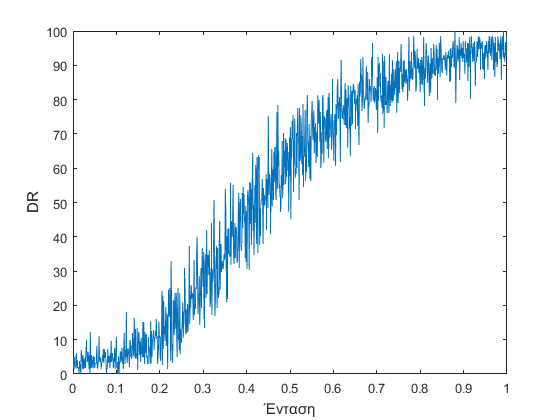
\includegraphics[width=70mm, height=50mm]{../../plots/gr_bigres_dr_intensity.png}
\caption{\en{DR} συναρτήσει της έντασης της κλοπής}
\label{fig:linearDRintensity}
\end{subfigure}
\quad
\begin{subfigure}[b]{0.4\textwidth}
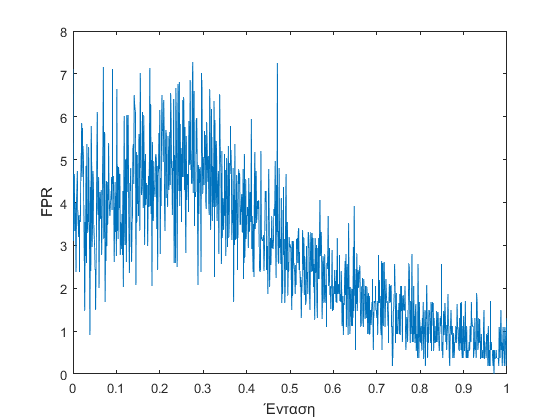
\includegraphics[width=70mm, height=50mm]{../../plots/gr_bigres_fpr_intensity.png}
\caption{\en{FPR} συναρτήσει της έντασης της κλοπής}
\label{fig:linearFPRintensity}
\end{subfigure}
\caption{Επίπτωση της έντασης στα αποτελέσματα}
\label{fig:linearintensityres}
\end{figure}
\newpage
\subsection{Ημερήσια ταξινόμηση με πυρήνα \en{RBF}}
\label{sec:RBFkernel}
Σε αυτή τη φάση δημιουργήθηκε η ανάγκη για εξαγωγή χαρακτηριστικών, ώστε να μειωθούν οι διαστάσεις των πινάκων και να επιταχυνθεί η διαδικασία. Παράλληλα, τα χαρακτηριστικά παρέχουν ένα επίπεδο αποπροσωποποίησης δημιουργώντας ένα αποτύπωμα της καταναλωτικής συνήθειας \cite{giwrgis}. Μετρώντας τα αθροίσματα, τα ελάχιστα, τα μέγιστα και τους μέσους όρους των καθημερινών καταναλώσεων δημιουργείται ένας βασικός κορμός χαρακτηριστικών για κάθε καταναλωτή που μπορεί εύκολα να επεκταθεί και σε άλλα γραμμικά και μη εξαρτώμενα χαρακτηριστικά.
\begin{itemize}
\item \textit{Μέγιστο και ώρα μεγίστου}
\item \textit{Ελάχιστο και ώρα ελαχίστου}
\item \textit{Άθροισμα κατανάλωσης ανά ημέρα}
\item \textit{Μέσος όρος, διακύμανση και τυπική απόκλιση ανά ημέρα}
\item \textit{Παράγοντας φορτίου, ελάχιστο προς μέση τιμή, ελάχιστο προς μέγιστο}
\item \textit{Επίδραση βραδινής κατανάλωσης}
\item \textit{Λοξότητα και Κύρτωση}
\end{itemize}
\par Η πρώτη δοκιμή του \en{SVM} έγινε με επιλογή 300 τυχαίων καταναλωτών μιας περιοχής με σκοπό να εκπαιδευτεί το σύστημα, ώστε να μπορεί να αναγνωρίζει ημέρες απάτης μέσα στο έτος. Η εκπαίδευση του ταξινομητή έγινε με τα ημερήσια χαρακτηριστικά για κάθε καταναλωτή. Τα δεδομένα διαχωρίζονται σε 2 τμήματα, το τμήμα της εκπαίδευσης που περιέχει 70\% του δείγματος των καταναλωτών και το τμήμα της δοκιμής που περιέχει ένα ποσοστό της τάξης του 30\% από το ίδιο δείγμα.\par
Ο ταξινομητής, λοιπόν, εκπαιδεύεται με ημερήσια χαρακτηριστικά κάθε καταναλωτή, αλλά θα πρέπει να αποφανθεί στο τέλος αν ο καταναλωτής έχει νοθεύσει τις μετρήσεις του ή όχι. Η λύση δόθηκε εισάγοντας ένα όριο ημερών το οποίο, αν ο ταξινιμητής το προσπερνούσε, τότε ο καταναλωτής θεωρείται πως έχει αλλοιώσει τα δεδομένα του. Για να βρούμε την βέλτιστη τιμή αυτού του ορίου, χρησιμοποιήθηκαν \en{ROC} καμπύλες για να παρατηρηθεί η μεταβολή του \en{DR} και \en{FPR}, ενώ αλλάζει το όριο ημερών.\\
\subsubsection{Αποτελέσματα δοκιμής}
Ελέγχοντας τα αποτελέσματα του Πίνακα \ref{tab:ROC50data}, παρατηρείται πως επιλέγοντας όριο στις 10 ημέρες επιτυγχάνεται ακρίβεια της τάξης του 95\% στην εύρεση της απάτης, αλλά με σχετικά υψηλό ποσοστό λάθος συναγερμού της τάξης του 15\% για τις έντονες απάτες. Αν χρειαστεί να ελαχιστοποιηθεί το \en{FPR}, θα πρέπει να επιλεχθεί μια μεγαλύτερη οριακή τιμή όπως το 14, που έχει ικανοποιητικό ποσοστό και στο \en{DR} που είναι της τάξης του 85\% και στο \en{FPR} που είναι της τάξης του 8\%. Οι απάτες που έγιναν με μικρότερη ένταση δεν γίνονται αντιληπτές από τον ταξινομητή που παράγει καμπύλη με παρόμοια κλίση με αυτή της ευθείας αναφοράς $y=x$.\par
Αντίστοιχα, στον Πίνακα \ref{tab:ROC35data} φαίνεται πως η μείωση του ποσοστού απάτης (\en{FR}) επηρέασε το σύστημα, και ειδικότερα μείωσε το όριο στις 10 μέρες με \en{DR}=85\% και \en{FPR}=9\%. Ουσιαστικά φαίνεται πως το σύστημα χρειάζεται και άλλους καταναλωτές, ώστε να αποτυπωθούν και οι καμπύλες για χαμηλότερες εντάσεις διείσδυσης στα δεδομένα. 

\begin{figure}[ht!]
\centering
\includegraphics[width=140mm, height=100mm]{../../plots/ROC50_1.png}
\caption{Καμπύλη \en{ROC} για \en{FR}=0.50 \label{fig:ROC50}}
\end{figure}

\begin{table}[ht!]
\begin{center}
\begin{tabular}{ |c|c|c|c|c|  }
 \hline
 \multicolumn{5}{|c|}{\en{300 IDs, 0.5 rate, 0-100 threshold}} \\
 \hline
 Όριο (Μέρες)    & \en{DR} (0.8) & \en{FPR} (0.8) & \en{DR} (0.5) & \en{FPR} (0.5) \\
 \hline
2 &	 97,917 &	40,385 &	76,712 &	35,0649\\
4 &	 97,143 &	25,625 & 	65,972 &	22,436\\
6 &	 95,683 &	22,360 &	54,225 &	13,924\\
8 &	 95,588 &	16,463 &	45,588 &	6,098\\
10 & 96,241 &	13,772 &	37,879 &	3,571\\
12 & 90,698 &	10,526 &	31,783 &	1,17\\
14 & 86,614 &	8,671  &	26,190 &	1,149\\
16 & 84,8	&	5,714  &	19,355 &	0\\
18 & 82,787 &	6,18   &	15,702 &	0\\
20 & 79,832 &	5,525  &	11,667 &	0\\
\hline
\end{tabular}
\end{center}
\caption{Πίνακας επιλογής ορίου \en{FR}=0.5 \label{tab:ROC50data}}
\end{table}

\begin{figure}[ht!]
\centering
\includegraphics[width=140mm, height=100mm]{../../plots/ROC35.png}
\caption{Καμπύλη \en{ROC} για \en{FR}=0.35 \label{fig:ROC35}}
\end{figure}
\clearpage
\begin{table}[ht!]
\begin{center}
\begin{tabular}{ |c|c|c| }
 \hline
 \multicolumn{3}{|c|}{\en{300 IDs, 0.35 rate, 0-100 threshold}} \\
 \hline
 Όριο (Μέρες)   & \en{DR} (0.8) & \en{FPR} (0.8)\\
 \hline
2 &	 95,192 &	30,612\\
4 &	 91,176 &	23,232\\
6 &	 89,691 &	17,734\\
8 &	 85,567 &	12,808\\
10 & 85,106 &	8,738\\
12 & 84,444 &	5,238\\
14 & 79,545 &	2,830\\
16 & 75		&	2,830\\
18 & 68,235 &	2,791\\
20 & 63,529 &	2,791\\
\hline
\end{tabular}
\end{center}
\caption{Πίνακας επιλογής ορίου \en{FR}=0.35 \label{tab:ROC35data}}
\end{table}

\section{Σχόλια}
Συνοψίζοντας, καθίσταται σαφές πως μπορεί να χρησιμοποιηθεί επιτυχώς επιβλεπόμενη μάθηση για τον εντοπισμό μη τεχνικών απωλειών. Οι γραμμικοί ταξινομητές μπορούν να αναγνωρίσουν αξιόπιστα και γρήγορα τον πρώτο τύπο απάτης, ενώ έχουν δυσκολία εντοπισμού στους υπόλοιπους τύπους. Παρ' όλα αυτά, χρησιμοποιώντας τον πυρήνα \en{RBF}, γίνεται εφικτή η αναγνώριση μη τεχνικών απωλειών αρχικά κάθε ημέρας και εν συνεχεία κάθε καταναλωτή. Γενικότερα, όμως, και οι δύο ομάδες ταξινομητών έχουν καλές επιδόσεις στον εντοπισμό ρευματοκλοπών με έντονη ένταση κλοπής, ενώ όσο μειώνεται η ένταση οι ταξινομητές δείχνουν μεγαλύτερη δυσκολία να διαχωρίσουν αλλοιωμένα από κανονικά δεδομένα.\par
Παράλληλα, γίνεται εμφανής η ανάγκη για σωστή επιλογή της δομής των δεδομένων εισόδου, καθώς κάθε ταξινομητής απαιτεί διαφορετική μεταχείριση. Οι γραμμικοί ταξινομητές απαιτούν πολλά χαρακτηριστικά (μετρήσεις), ενώ οι μη γραμμικοί μπορούν να λειτουργήσουν με πολύ λιγότερα. Αντίστοιχα, η κανονικοποίηση προσφέρει άμεση βελτίωση στα αποτελέσματα και επιταχύνει τη διαδικασία εκπαίδευσης σε μεγάλο βαθμό.

\chapter{Συστήματα μη επιβλεπόμενης μάθησης}
Ολοκληρώνοντας τον κύκλο των δοκιμών για τους αλγορίθμους επιβλεπόμενης μάθησης, δημιουργήθηκε η ανάγκη για περαιτέρω έρευνα σε διαφορετικούς αλγορίθμους. Οι αλγόριθμοι επιβλεπόμενης μάθησης έχουν ένα βασικό μειονέκτημα, όταν προσεγγίζεται ένα πραγματικό πρόβλημα. Αυτό είναι η δυσκολία εφαρμογής του αλγορίθμου, λόγω της έλλειψης των τάξεων των δεδομένων που απαιτεί ένα τέτοιο σύστημα για να εκπαιδευτεί. Η δυσκολία αυτή παρακάμπτεται, χρησιμοποιώντας μη επιβλεπόμενους ή ημι-επιβλεπόμενους αλγορίθμους που απαιτούν λίγα ή και κανένα ταξινομημένο παράδειγμα. Σε αυτό το κεφάλαιο θα προσεγγιστεί το πρόβλημα της ταξινόμησης καταναλωτών με νέα συστήματα που μπορούν να έχουν άμεσα χρήση στη λύση του πραγματικού προβλήματος, κάνοντας μια ανασκόπηση στις νέες δυσκολίες που προέκυψαν.
\section{Εξαγωγή Χαρακτηριστικών}
Στο παρόν μέρος θα γίνει παρουσίαση και ανάλυση των χαρακτηριστικών που χρησιμοποιήθηκαν στο μερικώς επιβλεπόμενο σύστημα, αλλά και στο μη επιβλεπόμενο σύστημα. Κάθε παράδειγμα μπορεί να περιγραφεί από ένα συνδυασμό τιμών που αναφέρονται ως μεταβλητές, χαρακτηριστικά, πεδία ή διαστάσεις. Οι τιμές αυτές μπορούν να είναι διαφορετικού τύπου όπως συνεχείς, δυαδικές ή κατηγορίες. Κάθε παράδειγμα μπορεί να αποτελείται μόνο από μια τιμή (μονοπαραγοντικό) ή και από περισσότερες (πολυπαραγοντικό). Στην περίπτωση των πολυπαραγοντικών παραδειγμάτων, όλες οι τιμές μπορεί να είναι ίδιου τύπου ή μπορεί να είναι ένας συνδυασμός διαφορετικών τύπων \cite{Anomaly}.\\
Παράλληλα, κάθε παράδειγμα μπορεί να οριστεί βάσει ακόμη δύο δομών ως προς τον ορισμό του προβλήματος \cite{Anomaly}.
\begin{enumerate}
\item{\textit{Τιμές Συσχετισμού}}: τέτοιου είδους τιμές χρησιμοποιούνται για να περιγράψουν ένα γενικό πλαίσιο που χαρακτηρίζει ένα παράδειγμα. Στις χρονοσειρές, ο χρόνος είναι μια τιμή που παρέχει μια σχετικότητα, η οποία καθορίζει τη θέση ενός παραδείγματος σε μια ολόκληρη ακολουθία. Μία τιμή γενικού πλαισίου είναι η μηνιαία κατανάλωση ενός κατοίκου.
\item{\textit{Συμπεριφορικές Τιμές}}: είναι οι τιμές που δεν προδίδουν ένα γενικό πλαίσιο για κάποιο παράδειγμα ή κάποια σχετικότητα. Ένα τέτοιο παράδειγμα θα μπορούσε να είναι η ετήσια παραγωγή ενέργειας σε όλο τον κόσμο.
\end{enumerate}
\subsection{Φύση Χαρακτηριστικών}
Το μερικώς επιβλεπόμενο και μη επιβλεπόμενο σύστημα απαιτούν εισόδους που να δίνουν τη δυνατότητα να διαχωρίζονται σε δύο κλάσεις οι καταναλωτές. Για να γίνει αυτό, απαιτείται η χρήση χαρακτηριστικών που αντιπροσωπεύουν την κλάση, αλλά και χαρακτηριστικών που προσδίδουν γενικότητα στο κάθε παράδειγμα. Με αυτό τον τρόπο, παρέχεται ένα περιθώριο στον αλγόριθμο, έτσι ώστε να μπορεί εύκολα να προσαρμόζεται σε καινούργια και ξεχωριστά παραδείγματα. Ένας απλοϊκός τρόπος να διαχωρίσουμε τα χαρακτηριστικά είναι σε γενικά και σε εξειδικευμένα χαρακτηριστικά για τον εντοπισμό κλοπής. Όλα τα παρακάτω χαρακτηριστικά αποτελούν τιμές συσχέτισης.
\subsubsection{Γενικά χαρακτηριστικά} 
Τα πλεονέκτημα των γενικών χαρακτηριστικών είναι ότι βοηθούν στην κατάταξη του καταναλωτή σε σχέση με τους υπόλοιπους, ώστε να εξαχθούν πληροφορίες, όπως ο τύπος καταναλωτή (οικιακού ή βιομηχανικού) και το προφίλ κατανάλωσής του. Τέτοια χαρακτηριστικά, όμως, πρέπει να περιορίζονται σε αριθμό, καθώς ενδέχεται να δυσκολεύσουν τον διαχωρισμό με βάση το κριτήριο που θέτουμε, παρέχοντας μεγάλο παράγοντα γενίκευσης. Τέτοιου είδους χαρακτηριστικά είναι τα παρακάτω:
\begin{enumerate}
\item{\textit{Ετήσια μέση τιμή ημίωρου}}: βρίσκεται ο μέσος όρος ημίωρου κάθε μέρας και ο ετήσιος μέσος όρος για όλες τις μέρες του έτους βρίσκεται.
\item{\textit{Ετήσια τυπική απόκλιση ημίωρου}}: βρίσκεται η τυπική απόκλιση κάθε μέρας και για όλες τις μέρες του έτους ο ετήσιος μέσος όρος της τυπικής απόκλισης.
\item{\textit{Διαφορά Ετήσιου Ελάχιστου τάσης με όμοιους}}: βάσει αυτού του χαρακηριστικού ορίζεται για όλους τους καταναλωτές το ελάχιστο της τάσης των χρονοσειρών τους και στη συνέχεια βρίσκεται η απόλυτη διαφορά σε ημέρες μεταξύ των συστάδων που δημιουργήθηκαν.
\item{\textit{Διαφορά μέσης τιμής με ομοίους}}: με αυτό το χαρακτηριστικό βρίσκεται η διαφορά του ετήσιου μέσου όρου κάθε καταναλωτή με την ομάδα καταναλωτών που ανήκει.
\item{\textit{Διαφορά τυπικής απόκλισης με ομοίους}}: με αυτό το χαρακτηριστικό βρίσκεται η διαφορά της ετήσιας τυπικής απόκλισης κάθε καταναλωτή με την ομάδα καταναλωτών που ανήκει.
\end{enumerate}
\subsubsection{Εξειδικευμένα χαρακτηριστικά}
Τα εξειδικευμένα χαρακτηριστικά επικεντρώνονται στην όξυνση των διαφορών μεταξύ των καταναλωτών διαφορετικών κλάσεων. Λειτουργούν, λοιπόν, σαν οδηγοί για τον αλγόριθμο, ώστε να κάνουν πιο εμφανείς τις διαφορές των κλάσεων. Το πλεονέκτημά τους είναι ο παράγοντας εξειδίκευσης που παρέχουν στον αλγόριθμο, διευκολύνοντάς τον να αναγνωρίζει με διαφορετικούς τρόπους κάθε κλάση. Το μειονέκτημα είναι πως λόγω της εξειδικευμένης τους φύσης μπορεί να μην εφαρμόζονται απόλυτα από όλους τους καταναλωτές ή στη χειρότερη περίπτωση να περιγράφουν μια σπάνια συμπεριφορά που δεν ενδιαφερόμαστε να διαχωρίσουμε.
\begin{enumerate}
\item{\textit{Κινούμενος μέσος όρος μηνιαίου μέσου όρου}}: πρόκειται για υπό συνθήκη χαρακτηριστικό, που αν παρατηρήσει κάποια σημαντική πτώση των καταναλώσεων, τότε ψάχνει για τη μέγιστη και την καταγράφει. Θεωρώντας ως $min$ τον μήνα του ελαχίστου και $c$ την κατανάλωση του αντίστοιχου $i$ μήνα, ορίζεται η εξής φόρμουλα για αυτό το χαρακτηριστικό. 
\begin{center}
\resizebox{8cm}{!}{$\bar{c_{p}}-\bar{c_{a}}=\frac{1}{k-1}\sum_{i=1}^{k} c_{m-i}-\frac{1}{w}\sum_{i=0}^{w}  c_{m+i}$}
\end{center}
\item{\textit{Κινούμενος μέσος όρος μηνιαίας τυπικής απόκλισης}}: πρόκειται για υπό συνθήκη χαρακτηριστικό, που αν παρατηρήσει κάποια σημαντική πτώση της τυπικής απόκλισης, τότε ψάχνει για την μέγιστη και την καταγράφει. Θεωρώντας ως $min$ τον μήνα του ελαχίστου και $std$ την τυπική απόκλιση της κατανάλωσης τον αντίστοιχο $i$ μήνα, ορίζεται η εξής φόρμουλα για αυτό το χαρακτηριστικό. 
\begin{center}
\resizebox{8.8cm}{!}{$\bar{std_{p}}-\bar{std_{a}}=\frac{1}{k-1}\sum_{i=1}^{k} std_{m-i}-\frac{1}{w}\sum_{i=0}^{w}  std_{m+i}$}
\end{center}
\item{\textit{Συμμετρική διαφορά καταναλώσεων}}: πρόκειται για υπό συνθήκη χαρακτηριστικό που παρατηρεί μια γενική συμπεριφορά όμοιων καταναλωτών ως προς τη χρονική στιγμή της ελάχιστης κατανάλωσης και ψάχνει για κάποια σημαντική πτώση της κατανάλωσης ανάμεσα σε δύο συμμετρικές χρονικές στιγμές με άξονα συμμετρίας την εκάστοτε χρονική στιγμή ελαχίστου. Θεωρώντας ως $min$ την ημέρα του ελαχίστου και $c$ την κατανάλωση της αντίστοιχης $i$ ημέρας ορίζονται οι εξής φόρμουλες εισάγοντας σε αυτό το σημείο και την ευκλείδεια απόσταση.
\begin{center}
\resizebox{8cm}{!}{$\bar{c_{p}}-\bar{c_{a}}=\frac{1}{n}\sum_{i=1}^{n+1} c_{min-i}-\frac{1}{n}\sum_{i=0}^{n}  c_{min+i}$}
\resizebox{9cm}{!}{$||c_{p}||-||c_{a}||=\sqrt{\sum_{i=1}^{n+1} (c_{min-i})^2}-\sqrt{\sum_{i=0}^{n}  (c_{min+i})^2}$}
\end{center}
\item{\textit{Συμμετρική διαφορά τυπικής απόκλισης}}: πρόκειται για υπό συνθήκη χαρακτηριστικό που παρατηρεί μια γενική συμπεριφορά όμοιων καταναλωτών ως προς τη χρονική στιγμή της ελάχιστης κατανάλωσης και ψάχνει για κάποια σημαντική πτώση της τυπικής απόκλισης ανάμεσα σε δύο συμμετρικές χρονικές στιγμές με άξονα συμμετρίας την εκάστοτε χρονική στιγμή ελαχίστου. Θεωρώντας ως $min$ την ημέρα του ελαχίστου και $std$ την τυπική απόκλιση της κατανάλωσης την αντίστοιχη $i$ ημέρα, ορίζεται η εξής φόρμουλα για αυτό το χαρακτηριστικό. 
\begin{center}
\resizebox{9cm}{!}{$\bar{std_{p}}-\bar{std_{a}}=\frac{1}{n}\sum_{i=1}^{n+1} std_{min-i}-\frac{1}{n}\sum_{i=0}^{n}  std_{min+i}$}
\resizebox{10cm}{!}{$||std_{p}||-||std_{a}||=\sqrt{\sum_{i=1}^{n+1} (std_{min-i})^2}-\sqrt{\sum_{i=0}^{n}  (std_{min+i})^2}$}
\end{center}
\item{\textit{Τμηματική διαφορά κατανάλωσης με όμοιους καταναλωτές}}: πρόκειται για υπό συνθήκη χαρακτηριστικό που παρατηρεί μια γενική συμπεριφορά όμοιων καταναλωτών ως προς τη χρονική στιγμή της ελάχιστης κατανάλωσης και ψάχνει για κάποια σημαντική πτώση της κατανάλωσης ανάμεσα στον καταναλωτή και τους ομοίους του μετά την χρονική στιγμή της ελάχιστης κατανάλωσης. Πιο φορμαλιστικά, θεωρώντας τον όρο $c_{cl}$ ως κατανάλωση μιας ομάδας και τον όρο $c_{co}$ ως κατανάλωση ενός πελάτη, έχουμε την παρακάτω διαφορά μέσων όρων και νορμών των καταναλώσεων.
\begin{center}
\resizebox{9cm}{!}{$\bar{c_{cl}}-\bar{c_{co}}=\frac{1}{n}\sum_{i=1}^{n+1} c_{cl,min-i}-\frac{1}{n}\sum_{i=0}^{n}  c_{co,min+i}$}
\resizebox{10cm}{!}{$||c_{cl}||-||c_{co}||=\sqrt{\sum_{i=1}^{n+1} (c_{cl,min-i})^2}-\sqrt{\sum_{i=0}^{n}  (c_{co,min+i})^2}$}
\end{center}
\item{\textit{Τμηματική διαφορά τυπικής απόκλισης με όμοιους καταναλωτές}}: πρόκειται για υπό συνθήκη χαρακτηριστικό που παρατηρεί μια γενική συμπεριφορά όμοιων καταναλωτών ως προς τη χρονική στιγμή της ελάχιστης κατανάλωσης και ψάχνει για κάποια σημαντική πτώση της τυπικής απόκλισης ανάμεσα στον καταναλωτή και τους όμοιούς του μετά την χρονική στιγμή της ελάχιστης κατανάλωσης. Πιο φορμαλιστικά θεωρώντας τον όρο $std_{cl}$ ως την τυπική απόκλιση κατανάλωσης μιας ομάδας και τον όρο $std_{co}$ την τυπική απόκλιση κατανάλωσης ενός πελάτη, έχουμε την παρακάτω διαφορά μέσων όρων και νορμών των τυπικών αποκλίσεων των καταναλώσεων.
\begin{center}
\resizebox{10cm}{!}{$\bar{std_{cl}}-\bar{std_{co}}=\frac{1}{n}\sum_{i=0}^{n}  std_{cl,min+i}-\frac{1}{n}\sum_{i=0}^{n}  std_{co,min+i}$}
\resizebox{11cm}{!}{$||std_{cl}||-||std_{co}||=\sqrt{\sum_{i=0}^{n} (std_{cl,min+i})^2}-\sqrt{\sum_{i=0}^{n}  (std_{co,min+i})^2}$}
\end{center}
\item{\textit{Χρονική Διαφορά Ελαχίστου}}: πρόκειται για υπό συνθήκη χαρακτηριστικό που εξερευνά το ελάχιστο χρονικό σημείο της τάσης της καμπύλης κάθε καταναλωτή. Με βάση την ομάδα που ανήκει κάθε καταναλωτής, υπολογίζεται η απόλυτη τιμή της χρονικής διαφοράς μεταξύ του ελαχίστου κάθε καταναλωτή με την ομάδα που ανήκει. Χρησιμοποιώντας ένα όριο για τη διαφορά αυτή, γίνεται αντιληπτή οποιαδήποτε έντονη διακύμανση του καταναλωτή με την ομάδα του και καταγράφεται σαν χαρακτηριστικό διαχωρισμού από την αναμενόμενη συμπεριφορά κατανάλωσης.
\begin{center}
\resizebox{3.5cm}{!}{$|t_{cl,min}-t_{co,min}|$}
\end{center}
\end{enumerate}

\subsection{Δοκιμή Χαρακτηριστικών με σταθερή απάτη}
Αφού οριστούν τα χαρακτηριστικά που εκτιμάται ότι μπορούν να βοηθήσουν στον διαχωρισμό των κλάσεων, έπεται φυσικά η δοκιμή τους με έναν απλό τρόπο, έτσι ώστε να επιβεβαιωθεί ότι μπορούν να λειτουργήσουν όπως αναμένεται. Παράλληλα, η δοκιμή αυτή παρέχει μεγάλο όγκο πληροφοριών, αφού καθιστά εμφανή τα σημεία και τις προϋποθέσεις τα οποία τα χαρακτηριστικά έχουν μεγάλη ακρίβεια, αλλά και αυτά στα οποία εκεί που υστερούν.\par
Ο κώδικας της δοκιμής θεωρεί δεδομένη και σταθερή την ένταση κλοπής και την ημέρα που κάθε καταναλωτής ξεκινά να αλλοιώνει τις τιμές του. Ειδικότερα, επιλέχθηκαν 2.000 καταναλωτές με το ποσοστό καταναλωτών που αλλοιώνει τις μετρήσεις του να είναι 50\%, η ένταση της κλοπής είναι της τάξης του 80\% και η μέρα κλοπής ορίζεται η 182η. Δηλαδή, μετά από 6 μήνες κανονικής κατανάλωσης ο χρήστης εισάγει σύστημα αλλοίωσης της μέτρησής του. Δοκιμάζοντας ξεχωριστά τα χαρακτηριστικά διαχωρισμού, ελέγχουμε το όριο κάθε χαρακτηριστικού, έτσι ώστε να δώσει μεγαλύτερη ακρίβεια στις επιθέσεις δεδομένων υπό τις παραπάνω συνθήκες. Αν  παρατηρηθούν τέτοια χαρακτηριστικά, ο καταναλωτής θεωρείται θετικός στην κλοπή. Αντίθετα, αν ο καταναλωτής δεν έχει την αναμενόμενη συμπεριφορά το χαρακτηριστικό δεν καταγράφει κάποια τιμή και ο καταναλωτής θεωρείται αρνητικός στην κλοπή. Αναλυτικότερα, για κάθε εξειδικευμένο χαρακτηριστικό λήφθηκαν τα παρακάτω αποτελέσματα:
\begin{enumerate}
\item{\textit{Κινούμενος μέσος όρος μηνιαίου μέσου όρου}} \\
Στην πρώτη δοκιμή δόθηκε έμφαση στη γενικότερη συμπεριφορά του χαρακτηριστικού ως προς το όριο που τίθεται κάθε φορά. Έτσι παρατηρείται εύκολα πως όταν το όριο είναι μεγάλο, ο διαχωρισμός παρουσιάζει χαμηλή ακρίβεια στον εντοπισμό με εξαιρετικά μικρό ποσοστό αστοχίας. Αντίθετα, αν το όριο χαμηλώσει αισθητά, χάνεται η έννοια του διαχωρισμού και ο αλγόριθμος θεωρεί θετικούς σε κλοπές σχεδόν όλους τους καταναλωτές.
\begin{center}
\begin{longtabu}  to 0.8\textwidth { | X[c] || X[c] | X[c] | X[c] | X[c] | X[c] |  }
 \hline
  Όριο & \en{DR}  & \en{FPR} & \en{BDR \%} & \en{Accuracy} & \en{F1}\\
 \hline
 0,8&	44,8&	1,4	&97	&71,7&	61,29\\
0,7&	98,7&	1,9	&98	&98,4&	98,4\\
0,6&	99,3&	3,6&	97&	97,85&	97,88\\
0,5&	99,8&	7,5	&93	&96,15&	96,15\\
0&	99,9&	91,5	&52	&54,2&	68,57\\
\hline
\caption{Δοκιμή 1ου χαρακτηριστικού}
\label{testfeat1}
\end{longtabu}
\end{center}

\item{\textit{Κινούμενος μέσος όρος μηνιαίας τυπικής απόκλισης}} \\
Αντίστοιχα, για παρόμοιες τιμές του ορίου με το προηγούμενο χαρακτηριστικό ο διαχωρισμός είναι εξαιρετικά εύστοχος και δεν αφήνει περιθώρια για αμφισβήτηση.
\begin{center}
\begin{longtabu} to 0.8\textwidth { | X[c] || X[c] | X[c] | X[c] | X[c] | X[c] |  }
 \hline
  Όριο & \en{DR}  & \en{FPR} & \en{BDR \%} & \en{Accuracy} & \en{F1}\\
 \hline
0,7	&98,2	&2,3	&98	&98,3	&98,31\\
0,6	&99,8	&4,1	&96	&97,85	&97,89\\
0,5	&99,5	&8,2	&92	&95,65	&95,81\\
\hline
\caption{Δοκιμή 2ου χαρακτηριστικού}
\label{testfeat2}
\end{longtabu}
\end{center}
\item{\textit{Συμμετρική διαφορά καταναλώσεων}} \\
Το συγκεκριμένο χαρακτηριστικό δεν δίνει αξιόπιστα αποτελέσματα, καθώς η συμμετρία που προκύπτει από τον χρησιμοποιούμενο τύπο απάτης κάνει το συγκεκριμένο χαρακτηριστικό να αποτυγχάνει σε αυτή τη δοκιμή. Παρ' όλα αυτά, το χαμηλό ποσοστό αστοχίας αφήνει δεύτερες σκέψεις, καθώς δεν επιβαρύνει αισθητά τα αποτελέσματα, αλλά βοηθά στη γενίκευση του τύπου κλοπής. 
\begin{center}
\begin{longtabu} to 0.8\textwidth { | X[c] || X[c] | X[c] | X[c] | X[c] | X[c] |  }
 \hline
  Όριο & \en{DR}  & \en{FPR} & \en{BDR \%} & \en{Accuracy} & \en{F1}\\
 \hline
 0,1&	26,3&	5,7&	82&	60,3&	39,85\\
\hline
\caption{Δοκιμή 3ου χαρακτηριστικού}
\label{testfeat3}
\end{longtabu}
\end{center}
Η δοκιμή συνεχίστηκε και με τις νόρμες των καταναλώσεων, παρουσιάζοντας ελάχιστη βελτίωση στο \en{DR}, ενώ αισθητά καλύτερα αποτελέσματα παρατηρούνται στο \en{FPR} που μειώθηκε ακόμη περισσότερο.
\begin{center}
\begin{longtabu} to 0.8\textwidth { | X[c] || X[c] | X[c] | X[c] | X[c] | X[c] |  }
 \hline
  Όριο & \en{DR}  & \en{FPR} & \en{BDR \%} & \en{Accuracy} & \en{F1}\\
 \hline
 0,3&	29&	2,1&	93&	63,65&	44,71\\
\hline
\caption{Δοκιμή 3ου χαρακτηριστικού με νόρμες}
\label{testfeat3norms}
\end{longtabu}
\end{center}

\item{\textit{Συμμετρική διαφορά τυπικής απόκλισης}} \\
Αντίστοιχα συμπεράσματα ισχύουν και στη συμμετρική διαφορά τυπικής απόκλισης που οριακά ξεπερνά το 10\% στο \en{FPR}. Η γενίκευση που προσφέρει ωστόσο το συγκεκριμένο χαρακτηριστικό είναι χρήσιμη, καθώς εν τέλει όλα τα χαρακτηριστικά θα ενώσουν τα δυνατά τους σημεία για να διαχωρίσουν απάτες με μεγαλύτερο τυχαίο παράγοντα.
\begin{center}
\begin{longtabu} to 0.8\textwidth { | X[c] || X[c] | X[c] | X[c] | X[c] | X[c] |  }
 \hline
  Όριο & \en{DR}  & \en{FPR} & \en{BDR \%} & \en{Accuracy} & \en{F1}\\
 \hline
 0,1&	38,9&	10,2&	79&	64,35&	52,18 \\
\hline
\caption{Δοκιμή 4ου χαρακτηριστικού}
\label{testfeat4}
\end{longtabu}
\end{center}
Σε αυτό το σημείο η μείωση του \en{FPR} είναι αρκετά σημαντικό ζήτημα που τελικώς επιτεύχθηκε με τις νόρμες που μπόρεσαν να μειώσουν το \en{FPR}, χωρίς να επηρεάσουν αρνητικά το \en{DR}. 
\begin{center}
\begin{longtabu} to 0.8\textwidth { | X[c] || X[c] | X[c] | X[c] | X[c] | X[c] |  }
 \hline
  Όριο & \en{DR}  & \en{FPR} & \en{BDR \%} & \en{Accuracy} & \en{F1}\\
 \hline
0,1&	40,2&	8,9&	82&	65,65&	53,92\\
\hline
\caption{Δοκιμή 4ου χαρακτηριστικού με νόρμες}
\label{testfeat4norms}
\end{longtabu}
\end{center}

\item{\textit{Τμηματική διαφορά κατανάλωσης με όμοιους καταναλωτές}} \\
Σε αυτό το χαρακτηριστικό παρατηρείται σχετική αστοχία σε σχέση με τα πρώτα χαρακτηριστικά, υποδεικνύοντας ανάγκη για καλύτερη ρύθμιση του χαρακτηριστικού. 
\begin{center}
\begin{longtabu} to 0.8\textwidth { | X[c] || X[c] | X[c] | X[c] | X[c] | X[c] |  }
 \hline
  Όριο & \en{DR}  & \en{FPR} & \en{BDR \%} & \en{Accuracy} & \en{F1}\\
 \hline
 0,1&	98,4&	11,4&	90&	93,5&	93,8\\
0,2&	93,9&	7&	93&	93,45	&93,48\\
0,3&	88,3&	4,9&	95&	91,7	&91,41\\
\hline
\caption{Δοκιμή 5ου χαρακτηριστικού}
\label{testfeat5}
\end{longtabu}
\end{center}
Δεδομένης της διαφοράς των καταναλώσεων, με τη γενικευμένη κατανάλωση μιας ομάδας δημιουργείται η ανάγκη για κανονικοποίηση σε κάθε διάνυσμα κατανάλωσης. Με αυτό τον τρόπο επιτυγχάνονται πολύ καλύτερα αποτελέσματα.
\begin{center}
\begin{longtabu} to 0.8\textwidth { | X[c] || X[c] | X[c] | X[c] | X[c] | X[c] |  }
 \hline
  Όριο & \en{DR}  & \en{FPR} & \en{BDR \%} & \en{Accuracy} & \en{F1}\\
 \hline
 0,3&	98,9&	5,4&	95&	96,75&	96,82\\
\hline
\caption{Δοκιμή 5ου χαρακτηριστικού με κανονικοποίηση}
\label{testfeat5normalized}
\end{longtabu}
\end{center}

\begin{center}
\begin{longtabu} to 0.8\textwidth { | X[c] || X[c] | X[c] | X[c] | X[c] | X[c] |  }
 \hline
  Όριο & \en{DR}  & \en{FPR} & \en{BDR \%} & \en{Accuracy} & \en{F1}\\
 \hline
0,1&	98,7&	7&	93&	95,85&	95,96\\
0,2&	97,6&	4,4&96&	96,6&	96,63\\
\hline
\caption{Δοκιμή 5ου χαρακτηριστικού με κανονικοποίηση και νόρμες}
\label{testfeat5normalizednorms}
\end{longtabu}
\end{center}

\item{\textit{Τμηματική διαφορά τυπικής απόκλισης με όμοιους καταναλωτές}} \\
Αντίστοιχη μεθοδολογία εφαρμόστηκε και σε αυτό το χαρακτηριστικό. Τα αποτελέσματα ήταν ικανοποιητικά, αλλά όχι αρκετά. Έτσι, χρησιμοποιήθηκε κανονικοποίηση, για μπορέσει να μειωθεί το \en{FPR}, ενώ αυξάνεται το \en{DR}.
\begin{center}
\begin{longtabu} to 0.8\textwidth { | X[c] || X[c] | X[c] | X[c] | X[c] | X[c] |  }
 \hline
  Όριο & \en{DR}  & \en{FPR} & \en{BDR \%} & \en{Accuracy} & \en{F1}\\
 \hline
 0,1&	99,4&	16,1&	86&	91,65&	92,25\\
0,2&	95,7&	8,3&	92&	93,7&	93,82\\
0,3&	89,8&	6,2&	94&	91,8&	91,63\\
\hline
\caption{Δοκιμή 6ου χαρακτηριστικού}
\label{testfeat6}
\end{longtabu}
\end{center}

\begin{center}
\begin{longtabu} to 0.8\textwidth { | X[c] || X[c] | X[c] | X[c] | X[c] | X[c] |  }
 \hline
  Όριο & \en{DR}  & \en{FPR} & \en{BDR \%} & \en{Accuracy} & \en{F1}\\
 \hline
 0,4&	97&	4,9&	95&	96,05&	96,09\\
0,3	&96,3&	5,3&	95&	95,5&	95,54\\
\hline
\caption{Δοκιμή 6ου χαρακτηριστικού με κανονικοποίηση}
\label{testfeat6normalized}
\end{longtabu}
\end{center}
\begin{center}
\begin{longtabu} to 0.8\textwidth { | X[c] || X[c] | X[c] | X[c] | X[c] | X[c] |  }
 \hline
  Όριο & \en{DR}  & \en{FPR} & \en{BDR \%} & \en{Accuracy} & \en{F1}\\
 \hline
0,2&	98,5&	4,5&	96&	97&	97,04\\
0,1&	99,2&	5,3&	95&	96,95&	97,02\\
\hline
\caption{Δοκιμή 6ου χαρακτηριστικού με κανονικοποίηση και νόρμες}
\label{testfeat6normalizednorms}
\end{longtabu}
\end{center}

\item{\textit{Χρονική Διαφορά Ελαχίστου}} \\
Δοκιμάζοντας το μοναδικό χαρακτηριστικό που σχετίζεται με χρόνο και όχι με κατανάλωση, καθίσταται σαφές πως δεν δίνει περισσότερη διακριτική ικανότητα στις κλάσεις. Αντίθετα, παρέχει μεγάλη γενικότητα στον αλγόριθμο, δίνοντας μια ακόμη πληροφορία για τη συμπεριφορά κατανάλωσης, αλλά λόγω του αισθητά μεγάλου \en{FPR} αποτυγχάνει να διαχωρίσει.
\end{enumerate}
\newpage
\begin{center}
\begin{longtabu} to 0.8\textwidth { | X[c] || X[c] | X[c] | X[c] | X[c] | X[c] |  }
 \hline
  Όριο & \en{DR}  & \en{FPR} & \en{BDR \%} & \en{Accuracy} & \en{F1}\\
 \hline
0,1&	85,4&	94,7&	47&	45,35&	60,98\\
0,2&	74,9&	81,7&	48&	46,6&	58,38\\
0,3&	18,9&	56,4&	25&	31,25&	21,56\\
0,4&	13,7&	34& 	29&	39,85&	18,55\\
\hline
\caption{Δοκιμή 7ου χαρακτηριστικού με κανονικοποίηση}
\label{testfeat7normalized}
\end{longtabu}
\end{center}



\subsection{Δοκιμή Χαρακτηριστικών με μεταβλητή απάτη}
Τέλος, έγινε μια τελική δοκιμή στα χαρακτηριστικά, αυτή τη φορά με μεγαλύτερο τυχαίο παράγοντα. Η ένταση της κλοπής καθορίζεται από μια Βήτα κατανομή με παραμέτρους 6 και 3, ενώ η ημέρα που ξεκινά η κλοπή επιλέγεται από μια κανονική κατανομή με παραμέτρους 182,5 και 56,1538. Σε κάθε καταναλωτή που έχει επιλεχθεί για κλοπή επιβάλλονται διαφορετικές τιμές των παραπάνω κατανομών κρατώντας όμως το γενικότερο πλαίσιο του τύπου της κλοπής που είδαμε προηγουμένως. Αυτό που έχει ενδιαφέρον να παρατηρηθεί σε αυτό το σημείο είναι το χαμηλό \en{FPR}, καθώς αναμένεται να χαμηλώσει σημαντικά η ακρίβεια λόγω της απλότητας του κανόνα διαχωρισμού.

\begin{center}
\begin{longtabu} to 0.8\textwidth { | X[c] | X[c] || X[c] | X[c] | X[c] | X[c] | X[c] |  }
 \hline
 Χαρακτ. & Όριο & \en{DR}  & \en{FPR} & \en{BDR \%} & \en{Accuracy} & \en{F1}\\
 \hline
1&	0,7&	42,8&	2,1&	95&	70,35&	59,08\\
2&	0,7&	46,5&	1,8&	96&	72,35&	62,71\\
3&	0,1&	58&		9,9&	85&	74,05&	69,09\\
4&	0,1&	59,6&	9,4&	86&	75,1&	70,53\\
5&	0,3&	66,4&	8,2&	89&	79,1&	76,06\\
6&	0,4&	58,4&	5,6&	91&	76,4&	71,22\\
7&	0,3&	48,8&	39,8&	55&	54,5&	51,75\\
\hline
\caption{Δοκιμή χαρακτηριστικών με τυχαίο παράγοντα}
\label{testfeatrandom}
\end{longtabu}
\end{center}


\begin{center}
\begin{longtabu} to 0.8\textwidth { | X[c] | X[c] || X[c] | X[c] | X[c] | X[c] | X[c] |  }
 \hline
 Χαρακτ. & Όριο & \en{DR}  & \en{FPR} & \en{BDR \%} & \en{Accuracy} & \en{F1}\\
 \hline
3&	0,3&	47,9&	2,9&	95&	72,65&	63,65\\
4&	0,1&	64,7&	10,5&	86&	77,1&	73,86\\
5&	0,1&	77,5&	8,8&	90&	84,35&	83,2\\
6&	0,1&	75,7&	7,9&	91&	83,9&	82,46\\
\hline
\caption{Δοκιμή χαρακτηριστικών με τυχαίο παράγοντα και νόρμες}
\label{testfeatrandomnorms}
\end{longtabu}
\end{center}

Καθίσταται, λοιπόν, σαφές πως τα χαρακτηριστικά σε γενικές γραμμές έχουν χαμηλότερη ακρίβεια, αλλά κρατούν χαμηλό \en{FPR} κάτι που μας ενδιαφέρει περισσότερο σε αυτό το σημείο. Παράλληλα, τα χαρακτηριστικά 3 και 4 που είχαν απογοητευτικά αποτελέσματα στην προηγούμενη δοκιμή, σε αυτήν δείχνουν να βελτιώνονται αισθητά σε σχέση με την επίδοση των υπολοίπων. Αυτό μας πληροφορεί ότι η αρχική υπόθεσή μας για το αίτιο αστοχία τους ήταν αληθής. Παράλληλα, το χαρακτηριστικό 7 που είχε επίσης εξαιρετικά αποθαρρυντικά αποτελέσματα στην προηγούμενη δοκιμή, εξισορροπεί σε αυτή τη δοκιμή τη σχέση μεταξύ του \en{DR} και \en{FPR}, παρόλο που ακόμη φαίνεται ως το χαρακτηριστικό με τα χειρότερα αποτελέσματα. 

\section{Aλγόριθμοι συσταδοποίησης}
Η συσταδοποίηση είναι από τους δημοφιλέστερους τύπου μη επιβλεπόμενης εκμάθησης. Σε αυτόν τον τύπο εκμάθησης, ο στόχος δεν είναι η ταξινόμηση των δεδομένων, αλλά απλά η εύρεση των ομοιοτήτων μεταξύ τους. Η υπόθεση είναι συνήθως πως οι συστάδες που ανακαλύπτονται θα ταιριάξουν σχετικά καλά με τη διαισθητική ταξινόμηση \cite{aihorizon}. Ειδικότερα ένα σύνολο παρατηρήσεων (σημείων δεδομένων) διαμερίζεται σε φυσικές ομαδοποιήσεις, ή συστάδες (\en{clusters}), με τέτοιο τρόπο ώστε το μέτρο ομοιότητας μεταξύ οποιουδήποτε ζεύγους παρατηρήσεων που αντιστοιχίζεται σε κάθε συστάδα να ελαχιστοποιεί μια καθορισμένη συνάρτηση κόστους.\par
\subsection{\en{K-Means}}
\label{doc:kmeans}
Δοθέντος ενός συνόλου $N$ παρατηρήσεων, ζητείται ο κωδικοποιητής $C$ που αντιστοιχίζει αυτές τις παρατηρήσεις στις $K$ συστάδες με τέτοιο τρόπο, ώστε μέσα σε μια συστάδα ο μέσος όρος του μέτρου ανομοιότητας των αντιστοιχισμένων παρατηρήσεων ως προς το κέντρο (μέσο) της συστάδας να ελαχιστοποιείται μέσω της συνάρτησης κόστους.
\begin{center}
$J(C)= \sum_{j=1}^K \sum_{C(i)=j}\|\mathbf{x}_i-\bar{\mathbf{\mu}_j}\|^2$
\end{center}
Με μαθηματικούς όρους, ο αλγόριθμος (\en{K-Means}) εξελίσσεται σε δύο βήματα:
\begin{enumerate}
\item Για ένα δεδομένο κωδικοποιητή $C$, η συνολική διακύμανση συστάδας ελαχιστοποιείται ως προς το σύνολο μέσων συστάδας $\{\bar{\mathbf{\mu}_j}\}_{j=i}^K$, δηλαδή εκτελούμε την ακόλουθη ελαχιστοποίηση:
\begin{center}
$ min_{\{\bar{\mu_j}\}_{j=i}^K} \sum_{j=i}^K \sum_{C(i)=j} \|\mathbf{x}_i-\bar{\mathbf{\mu}_j}\|^2$ για δεδομένο $C$
\end{center}
\item Αφού υπολογιστούν οι βελτιστοποιημένοι μέσοι συστάδας $\{\bar{\mathbf{\mu}_j}\}_{j=i}^K$, στη συνέχεια βελτιστοποιηούμε τον κωδικοποιητή ως εξής:
\begin{center}
$C(i) = arg min_{1 \leq j \leq K} \|\mathbf{x}_i-\bar{\mathbf{\mu}_j}\|^2$
\end{center}
\end{enumerate}
\par Ξεκινώντας από κάποια αρχική επιλογή κωδικοποιητή $C$, ο αλγόριθμος εναλλάσσεται μεταξύ αυτών των δύο βημάτων μέχρι να μην υπάρξει περαιτέρω αλλαγή στις αντιστοιχίσεις των συστάδων\cite{haykin}.
\subsection{\en{Fuzzy C-Means}}
Ο αλγόριθμος ασαφών \en{C} μέσων (\en{FCM}) είναι πολύ κοντά στη λογική του \en{K-Means}, αλλά εισάγει μια πιο πιθανοτική προσέγγιση. Επιλύει το πρόβλημα της ελαχιστοποίησης των αποστάσεων μέσα σε μια συστάδα και της μεγιστοποίησης των αποστάσεων μεταξύ των συστάδων με βάση το παρακάτω κριτήριο βελτιστοποίησης\cite{fuzzyclustering}:
\begin{center}
$J_m = \sum_{k=1}^N\sum_{i=1}^n(u_{ik})^m\|\mathbf{x}_k-v_i\|^2$
\end{center} 
Έστω ένα σύνολο διανυσμάτων δεδομένων $\mathbf{X}=\{\mathbf{x}_1, \mathbf{x}_2, ..., \mathbf{x}_3\}$ με $x_k \in \R^p$ ($1 \leq k \leq n$), τα οποία ομαδοποιούνται σε ασαφείς συστάδες.
\begin{enumerate}
\item Επιλογή αριθμού $c$ των ασαφών συστάδων, της παραμέτρου $m$, των αρχικών τιμών για τα διανύσματα  $\mathbf{v}_1, \mathbf{v}_2, ...,\mathbf{v}_c$ και της παραμέτρου $c$.
\begin{center}
    όπου $\mathbf{v}_i=\frac{\sum_{i=1}^n(u_{ik})^mx_{ik}}{\sum_{i=1}^n(u_{ik})}$
\end{center}
\item Χρήση της παρακάτω εξίσωσης για τον υπολογισμό των συναρτήσεων συμμετοχής $u_{ik}$
\begin{center}
$u_{ik}=\frac{1}{\sum_{j=1}^c (\frac{\|\mathbf{x}_k-\mathbf{v}_i\|}{\|\mathbf{x}_k-\mathbf{v}_j\|})}$, $(1 \leq k \leq n)$, $(1 \leq i \leq c)$
\end{center}
\item Βάσει της εξίσωσης του βήματος 1, γίνεται προσδιορισμός των νέων τιμών για τα κέντρα των ασαφών υποομάδων $\mathbf{v}_1^{new}, \mathbf{v}_2^{new}, ...,\mathbf{v}_c^{new}$
\item Αν $max_i\{\|\mathbf{v}_i-\mathbf{v}_i^{new}\|^2\}<\epsilon$ τότε ο αλγόριθμος σταματάει, αλλιώς θέτει $\mathbf{v}_i=\mathbf{v}_i^{new}$ και η ροή του πηγαίνει στο βήμα 2.

\end{enumerate}
\subsection{\en{SOM}}
Εμπνευσμένοι από τα νευρωνικά δίκτυα, οι αυτο-οργανωμένοι χάρτες (\en{SOM}) χρησιμοποιούν ένα μηχανισμό ανταγωνισμού και συνεργασίας για να πετύχουν μη επιβλεπόμενη εκμάθηση.  Στην κλασσική περίπτωση του \en{SOM}, ένα μέρος από κόμβους οργανώνεται σε γεωμετρικό σχήμα, συνήθως δισδιάστατο πλέγμα. Κάθε κόμβος σχετίζεται με ένα διάνυσμα βάρους με τις ίδιες διαστάσεις όπως η είσοδος. Ο σκοπός του \en{SOM} είναι να βρει μια χαρτογράφηση από τον υψηλό χώρο διαστάσεων της εισόδου σε δισδιάσταστη αναπαράσταση των κόμβων. Ένας τρόπος να χρησιμοποιηθεί για συσταδοποίηση είναι να αναμένεται τα αντικείμενα στον χώρο εισόδου να αναπαρασταθούν από τον ίδιο κόμβο, όπως σχηματίστηκαν στη συστάδα. Στη διάρκεια της εκπαίδευσης, κάθε αντικείμενο στην είσοδο αναπαριστάται στον χάρτη και αναγνωρίζεται ο κόμβος που ταιριάζει βέλτιστα. Τυπικά, όταν η είσοδος και τα διανύσματα βαρών κανονικοποιηθούν, για δείγμα εισόδου $x(t)$ ο νικητής δείκτης $c$ ορίζεται κάτω από τη συνθήκη:
\begin{center}
για όλα $i$, $\|x(t)-m_c(t)\| \leq \|x(t)-m_i(t)\|$
\end{center}
όπου $t$ είναι το χρονικό βήμα στην εκπαίδευση, $m_i$ είναι το διάνυσμα βάρους του $i$ κόμβου. Μετά από αυτό, το διάνυσμα βάρους γύρω από τον βέλτιστο κόμβο $c=c(x)$ ανανεώνεται ως εξής:
\begin{center}
 $m_i(t+1)=m_i(t)+\alpha h_{c(x),i}(x(t)-m_i(t))$
\end{center}
όπου $\alpha$ είναι ο ρυθμός εκμάθησης και $h_{c(x),i}$ είναι η «γειτονική συνάρτηση», μια φθίνουσα συνάρτηση μεταξύ $i$ και $c$ κόμβων στο δίκτυο του χάρτη \cite{clustercomparison}.
\section{Συστατικά συστήματος μη επιβλεπόμενης μάθησης}
Οι δοκιμές στην επιβλεπόμενη μάθηση έδειξαν πως η ταξινόμηση των συγκεκριμένων χρονοσειρών δεν είναι εύκολη διαδικασία. Για αυτό το λόγο, χρησιμοποιήθηκε συστοιχία μη επιβλεπόμενων αλγορίθμων για την ταξινόμηση των καταναλωτών. Ειδικότερα, εισήχθη ένα σύστημα με ταξινόμηση βάσει κανόνων, το οποίο συσταδοποιεί τα δεδομένα και εξάγει χαρακτηριστικά των χρονοσειρών και αποτελέσματα, λαμβάνοντας υπόψη τα παραπάνω. Η βέλτιστη δομή του συστήματος επιτεύχθηκε, όπως φαίνεται στο Σχήμα \ref{fig:unsupervisedsystem}.\par
\begin{figure}[ht!]
\centering
 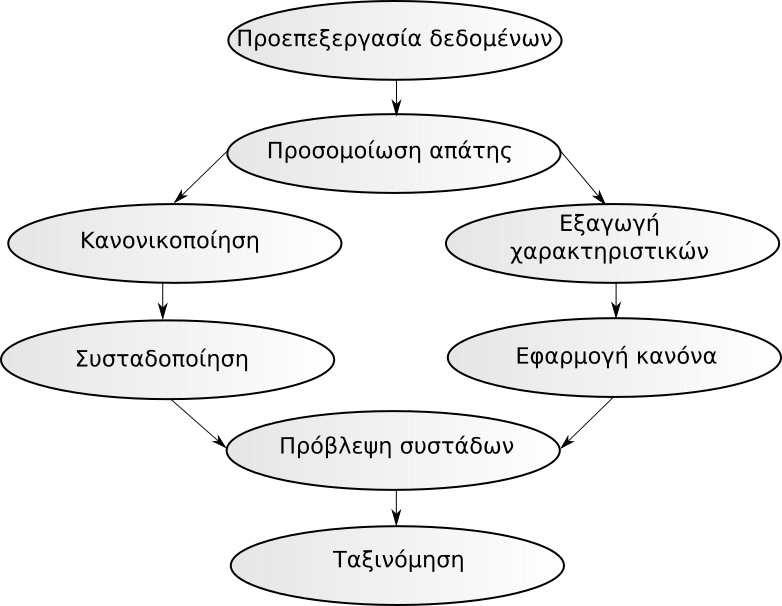
\includegraphics[width=90mm, height=60mm]{../../plots/systems/un_supervised.png}
 \caption{Δομή μη επιβλεπόμενου ταξινομητή}
\label{fig:unsupervisedsystem}
 \end{figure}
Παρέχοντας περαιτέρω πληροφορίες για τα μέλη που απαρτίζουν το σύστημα προς έρευνα, έχουμε:
\begin{itemize}
\item \textit{Προεπεξεργασία δεδομένων}: επιλέγονται και οργανώνονται τα δεδομένα σε συγκεκριμένους πίνακες και διανύσματα.
\item \textit{Προσομοίωση απάτης}: αλλοιώνονται οι μετρήσεις κάποιων καταναλωτών και ενημερώνονται οι προϋπάρχοντες πίνακες και διανύσματα.
\item \textit{Κανονικοποίηση}: κανονικοποιούνται οι ετήσιες χρονοσειρές κάθε καταναλωτή σε εύρος τιμών [-1,1].
\item \textit{Συσταδοποίηση}: συσταδοποιούνται οι καταναλωτές με βάση τις κανονικοποιημένες τιμές σε δύο συστάδες. Η μια συστάδα ομαλή και η άλλη ανώμαλη. 
\item \textit{Εξαγωγή χαρακτηριστικών}: βάσει των χρονοσειρών δημιουργούνται ετήσια χαρακτηριστικά για κάθε καταναλωτή, προσπαθώντας να ανιχνευθεί ύποπτη συμπεριφορά.
\item \textit{Εφαρμογή κανόνα}: απενοχοποιούνται κάποιοι καταναλωτές που βρίσκονται στην ανώμαλη συστάδα λαμβάνοντας υπόψη το πλήθος των χαρακτηριστικών.
\item \textit{Πρόβλεψη συστάδων}: ορίζονται κλάσεις στις συστάδες με σεβασμό στον κανόνα.
\item \textit{Ταξινόμηση}: ταξινομούνται οι καταναλωτές και παράγονται τα τελικά αποτελέσματα και μετρικές.
\end{itemize}

 
\subsection{Μεθοδολογία εξαγωγής αποτελεσμάτων}
Η εξαγωγή αποτελεσμάτων διαδραματίζει μεγάλο ρόλο στην τελική απόδοση του αλγορίθμου, οπότε χρειάζεται ιδιαίτερη προσοχή στην τοποθέτηση δυαδικών χαρακτηριστικών. Η γενικότερη μεθοδολογία βασίζεται σε δύο σημαντικούς άξονες, καθώς η τομή των δύο είναι αυτή που εξάγει τα βέλτιστα αποτελέσματα. Αυτό γίνεται ξεκάθαρο παρατηρώντας τον πίνακα αποτελεσμάτων \ref{tab:testrules}.\par
Ο πρώτος άξονας αποτελείται από την κανονικοποίηση και τη συσταδοποίηση. Κατά την διαδικασία της κανονικοποίησης, o πίνακας με τις χρονοσειρές αναστρέφεται, κανονικοποιείται και αναστρέφεται για δεύτερη φορά για να αποκτήσει την ίδια μορφή με την αρχική, αλλά με εύρος τιμών [-1,1]. Με αυτό τον τρόπο, δίνεται έμφαση στη μορφή και όχι στα μεγέθη των χρονοσειρών. Έτσι, το σύστημα εκμεταλλεύεται το γεγονός ότι οι χρονοσειρές είναι αρκετά ομοιόμορφες ως προς το σχήμα. Σε επόμενη φάση εκτελείται συσταδοποίηση στα κανονικοποιημένα μεγέθη και διαχωρίζονται οι καταναλωτές σε μια μεγάλη συστάδα με αναμενόμενες μορφές και σε μια μικρή συστάδα με ακανόνιστες συμπεριφορές.\par
Ο δεύτερος άξονας αποτελείται από την εξαγωγή χαρακτηριστικών των χρονοσειρών και την εφαρμοφή του κανόνα. Η εξαγωγή δίνει τη δυνατότητα μέσω των χαρακτηριστικών διαχωρισμού να δημιουργηθούν ομάδες καταναλωτών που έχουν ύποπτες και αναμενόμενες μετρήσεις. Αν έχουμε έλλειψη χαρακτηριστικών, δηλαδή $0$, πρακτικά σημαίνει πως ο καταναλωτής έχει αναμενόμενη συμπεριφορά. Στην αντίθετη περίπτωση ο καταναλωτής έχει αποκλίνουσα συμπεριφορά και θεωρείται ύποπτος. Εκεί εφαρμόζεται ο κανόνας που ορίζει πως αν ο καταναλωτής έχει λιγότερες από τρεις μετρήσεις στα χαρακτηριστικά διαχωρισμού, η συμπεριφορά του θεωρείται αναμενόμενη.\par
Για τη δοκιμή των κανόνων επιλέχθηκε δείγμα 2.000 καταναλωτών με ποσοστό διείσδυσης μη τεχνικών απωλειών στο 10\%. Έγιναν συνολικά τρεις δοκιμές για τους κανόνες, με τον πρώτο να ελέγχει την απόδοση της συσταδοποίησης, τον δεύτερο να ελέγχει την απόδοση των χαρακτηριστικών και τον τρίτο να ελέγχει τον συνδυασμό των δύο κανόνων.\par
\begin{center}
\begin{longtabu} to 0.8\textwidth { | X[c] || X[c] | X[c] | X[c] | X[c] | X[c] |  }
 \hline
 Κανόνας& \en{DR}  & \en{FPR} & \en{Accuracy} & \en{F1 score} & \en{BDR \%}\\
\hline
 Συσταδ. & 98.67	&	34.2 &	69.09 &	38.96 &	24\\
\hline
 Χαρακτ.& 87.78	&	6.72 &	92.73 &	70.73 &	59\\ 
 \hline
 Συνδ. & 89.33	&	5.93 &	93.6 &	73.63 &	63\\
\hline
\caption{Δοκιμή στους κανόνες}
\label{tab:testrules}
\end{longtabu}
\end{center}

\section{Δοκιμή συστήματος μη επιβλεπόμενης μάθησης}
Για να επιβεβαιωθεί η ορθή και βέλτιστη λειτουργία του συστήματος, απαιτείται δοκιμή των παραμέτρων που το απαρτίζουν. Για να συμβεί αυτό, επιλέχθηκαν 4.500 καταναλωτές και αλλοιώθηκαν τα δεδομένα μόνο του 10\%. Ο τύπος απάτης που χρησιμοποιήθηκε για την αλλοίωση των δεδομένων είναι ο πρώτος, καθώς φάνηκε πως είναι ιδιαίτερα πολύπλοκο ακόμη και για επιβλεπόμενο σύστημα να παράξει αξιόπιστα αποτελέσματα στους υπόλοιπους τύπους απάτης. Παράλληλα, έγινε μια ακόμη δοκιμή μη επιβλεπόμενου συστήματος εξερευνώντας τις δυνατότητες της ασαφούς συσταδοποίησης \en{FCM}.\par

\subsection{Αποτελέσματα δοκιμής συστήματος}
Παρατηρώντας το Σχήμα \ref{fig:unsupDRintensity}, μπορούμε να παρατηρήσουμε πως έχουμε ομαλή αύξηση του \en{DR} μετά το 0.5, ενώ αντίστοιχα έχουμε ομαλή μείωση του \en{FPR} μετά το ίδιο σημείο. Πριν από το σημείο αυτό, οι κυματομορφές έχουν σχετική ασυνέπεια στα αποτελέσματα, κάνοντας βίαιες αλλαγές στις μετρικές τους. Πιο συγκεκριμένα, στο εύρος [0.4, 0.5] εμφανίζονται δύο μεγάλα πλήγματα στην επίδοση του συστήματος που προδίδουν πως υπό κάποιες συνθήκες το σύστημα δυσκολεύεται να ορίσει την κλοπή, χωρίς όμως να ενοχοποιεί αδίκως.\par

\begin{figure}[ht!]
\centering
\begin{subfigure}[b]{0.4\textwidth}
 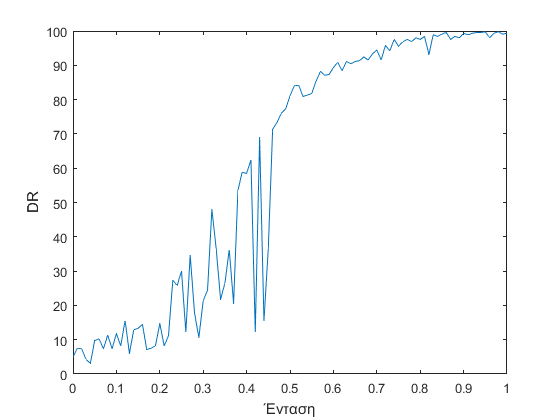
\includegraphics[width=70mm, height=50mm]{../../plots/gr_bigres_dr_intensity_un_sup.png}
\caption{\en{DR} συναρτήσει της έντασης της κλοπής}
\label{fig:unsupDRintensity}
\end{subfigure}
\quad
\begin{subfigure}[b]{0.4\textwidth}
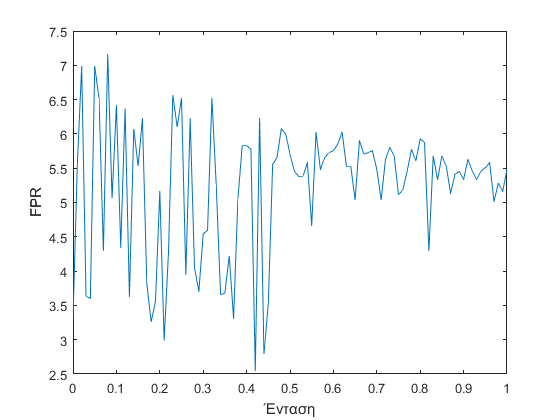
\includegraphics[width=70mm, height=50mm]{../../plots/gr_bigres_fpr_intensity_un_sup.png}
\caption{\en{FPR} συναρτήσει της έντασης της κλοπής}
\label{fig:linearFPRintensity}
\end{subfigure}
\caption{Επίπτωση της έντασης στα αποτελέσματα}
\label{fig:unsupintensityres}
\end{figure}

Παράλληλα, αξίζει να σημειωθεί εδώ πως οι αλγόριθμοι συσταδοποίησης μπορούν να αλλάξουν σε κάποιο βαθμό τα χαρακτηριστικά του συστήματος και την επίδοσή του. Ως αποτέλεσμα, έγινε δοκιμή για τους διαφορετικούς αλγορίθμους που χρησιμοποιήθηκαν στην εξαγωγή των χαρακτηριστικών, καταλήγοντας σε αποτελέσματα για κάθε περίπτωση.
\newpage
\begin{center}
\begin{longtabu} to 0.8\textwidth { | X[c] || X[c] | X[c] | X[c] | X[c] | X[c] |  }
 \hline
 Αλγ.& \en{DR}  & \en{FPR} & \en{Accuracy} & \en{F1 score} & \en{BDR \%}\\
\hline
 \en{K-Means} & 86.44	&	5.43 &	93.76 &	73.47 &	64\\
\hline
 \en{SOM}& 89.11	&	5.23 &	94.2 &	75.45 &	65\\ 
 \hline
  \en{Fuzzy} & 85.78	&	4.99 &	94.09 &	74.37 &	66\\
\hline
\caption{Εξερεύνηση συσταδοποιήσεων χαρακτηριστικών στο μη-επιβλεπόμενο σύστημα}
\label{tab:testclusterunsup}
\end{longtabu}
\end{center}
\par Γίνεται, λοιπόν, αντιληπτό πως οι αλγόριθμοι συσταδοποίησης στην εξαγωγή δεδομένων παίζουν σχετικά μικρό ρόλο, αφού τα αποτελέσματα έχουν πολύ μικρές αποκλίσεις μεταξύ τους. Αυτό ήταν κάτι αναμενόμενο βέβαια, καθώς μόνο δύο από τα οκτώ χαρακτηριστικά έχουν άμεση συσχέτιση με τη συσταδοποίηση.\par
\subsection{Εξερεύνηση δυνατοτήτων \en{FCM}}
Ο αλγόριθμος ασαφών $C$ μέσων μέσα από τον παράγοντα ασάφιας δίνει τη δυνατότητα να εξερευνηθούν οι συστάδες και με διαφορετικούς τρόπους. Ειδικότερα, ο παράγοντας αυτός καθορίζει την επικάλυψη των συστάδων και στη συγκεκριμένη δοκιμή επιλέχθηκε παράγοντας ασάφειας 3 με το 1 να αντιστοιχεί σε συσταδοποίηση χωρίς επικαλύψεις. Παράλληλα, για να μπορέσει να διευκρινιστεί τελικά πού ανήκει κάθε παράδειγμα, παρέχεται μια τιμή για παράδειγμα με τη μεγαλύτερη από αυτή να υποδηλώνει μεγάλο βαθμό ομοιότητας του παραδείγματος με τη συστάδα.\par
Με αυτό το σκεπτικό δημιουργήθηκε μια δοκιμή με 4.500 καταναλωτές και 10\% διείσδυση μη τεχνικών απωλειών κατά την οποία ταξινομούνται οι καταναλωτές χωρίς εξαγωγή χαρακτηριστικών. Ειδικότερα, γνωρίζοντας σε αδρές γραμμές το ποσοστό των απατών, τίθεται ένα όριο στο πλήθος που επιθυμεί κάποιος να ελέγξει. Ο αλγόριθμος βάσει αυτού του πλήθους επιλέγει το δείγμα των καταναλωτών που φαίνεται πιο σίγουρο ότι ανήκει στη συστάδα με ακανόνιστες μετρήσεις. Στην πράξη, αν από 450 κλοπές τεθεί ένα όριο στην εύρεση μόνο των 100, ο αλγόριθμος έχει τη δυνατότητα να αναγνωρίσει σωστά 81, ενώ λάθος 19, όπως φαίνεται και στο Σχήμα \ref{fig:wrongpredFCM}.\par
Πρακτικά, για να συμβεί αυτό ταξινομούνται σε αύξουσα σειρά οι καταναλωτές με το μεγαλύτερο ποσοστό συμμετοχής στην ακανόνιστη συστάδα. Έτσι, οι πιο ανώμαλες καταναλωτικές συμπεριφορές έχουν προτεραιότητα στον έλεγχο και καθίσταται δυνατό να οριστεί ένα όριο χαμηλότερο από τις συνολικές απώλειες για έλεγχό τους βάσει της ταξινόμησης, εμπνέοντας μεγαλύτερο βαθμό σιγουριάς.\par
\begin{figure}[ht!]
\centering
 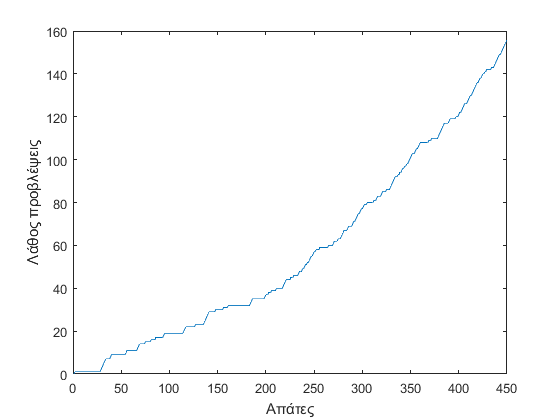
\includegraphics[width=70mm, height=50mm]{../../plots/confident_predictions.png}
\caption{Καμπύλη λάθος προβλέψεων με \en{FCM}}
\label{fig:wrongpredFCM}
\end{figure}
\newpage
\section{Συστατικά συστήματος ημι-επιβλεπόμενης μάθησης}
Η ημι-επιβλεπόμενη προσέγγιση του προβλήματος επιτυγχάνεται εισάγοντας στο σύστημα μη επιβλεπόμενης μάθησης νέους αλγορίθμους. Με αυτό τον τρόπο αποκτάται η δυνατότητα εκπαίδευσης με ένα μικρό δείγμα καταναλωτών και των δύο τάξεων ή με μεγαλύτερο δείγμα καταναλωτών της αρνητικής τάξης. Έτσι, καλύπτονται και οι δύο δημοφιλέστερες προσεγγίσεις της ημι-επιβλεπόμενης μάθησης. Εν συνεχεία, βάσει του μοντέλου της εκπαίδευσης ταξινομούνται οι καταναλωτές. Παράλληλα, η προσθήκη νέων αλγορίθμων δίνει τη δυνατότητα εποπτείας των χαρακτηριστικών, αλλά και του μοντέλου που δημιουργήθηκε σε δισδιάστατο χώρο. Οπτικοποιούνται λοιπόν οι πληροφορίες και η εσωτερική λειτουργία του αλγορίθμου, ενώ παράλληλα παρέχεται η δυνατότητα εκπαίδευσης προτύπων.\par
\begin{figure}[ht!]
\centering
 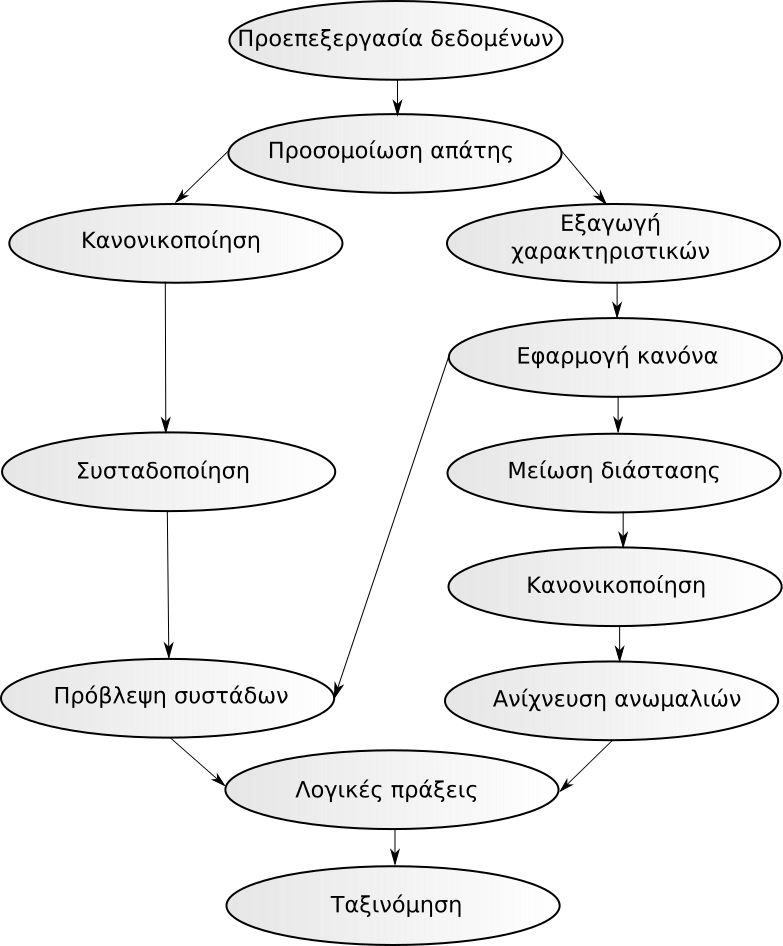
\includegraphics[width=90mm, height=100mm]{../../plots/systems/semi_supervised.png}
 \caption{Δομή ημι-επιβλεπόμενου ταξινομητή}
\label{fig:semisupervisedsystem}
 \end{figure}

Αναλυτικότερα, η δομή του αλγορίθμου αναπαρίσταται στο Σχήμα \ref{fig:semisupervisedsystem} ενώ αξίζει να γίνει μια εισαγωγή στα κομμάτια που απαρτίζουν το σύστημα:
\begin{itemize}
\item \textit{Προεπεξεργασία δεδομένων}: επιλέγονται και οργανώνονται τα δεδομένα σε συγκεκριμένους πίνακες και διανύσματα.
\item \textit{Προσομοίωση απάτης}: αλλοιώνονται οι μετρήσεις κάποιων καταναλωτών και ενημερώνονται οι προϋπάρχοντες πίνακες και διανύσματα.
\item \textit{Κανονικοποίηση}: κανονικοποιούνται οι ετήσιες χρονοσειρές και τα χαρακτηριστικά κάθε καταναλωτή σε εύρος τιμών [-1,1] και [0,1] αντίστοιχα.
\item \textit{Συσταδοποίηση}: συσταδοποιούνται οι καταναλωτές με βάση τις κανονικοποιημένες τιμές σε δύο συστάδες. Η μια συστάδα ομαλή και η άλλη η ανώμαλη. 
\item \textit{Εξαγωγή χαρακτηριστικών}: βάσει των χρονοσειρών δημιουργούνται ετήσια χαρακτηριστικά για κάθε καταναλωτή, με στόχο να ανιχνευθεί ύποπτη συμπεριφορά.
\item \textit{Εφαρμογή κανόνα}: απενοχοποιούνται κάποιοι καταναλωτές που βρίσκονται στην ανώμαλη συστάδα λαμβάνοντας υπόψη το πλήθος των χαρακτηριστικών .
\item \textit{Πρόβλεψη συστάδων}: προβλέπονται οι κλάσεις στις συστάδες με σεβασμό στον κανόνα.
\item \textit{Μείωση διάστασης}: ο πολυδιάστατος χώρος των χαρακτηριστικών μειώνεται σε χώρο δύο διαστάσεων.
\item \textit{Ανίχνευση ανωμαλιών}: εκπαιδεύεται το μοντέλο πρόβλεψης βάσει των χαρακτηριστικών και βελτιστοποιούνται τα όρια ταξινόμησης.
\item \textit{Λογικές πράξεις}: εκτελούνται λογικές πράξεις μεταξύ των δυαδικών χαρακτηριστικών που προέρχονται από την πρόβλεψη συστάδων και την ανίχνευση ανωμαλιών.
\item \textit{Ταξινόμηση}: ταξινομούνται οι καταναλωτές και παράγονται τα τελικά αποτελέσματα και μετρικές.
\end{itemize}

\subsection{Θεωρία αλγορίθμου μείωσης διάστασης}
Το \en{PCA} είναι ένας μη επιβλεπόμενος αλγόριθμος γραμμικής μείωσης διάστασης που στοχεύει στην εύρεση μιας βάσης ή ενός συστήματος συντεταγμένων με περισσότερο νόημα για τα δεδομένα και λειτουργεί βάσει του πίνακα συνδιακύμανσης για την εύρεση ισχυρών χαρακτηριστικών.\par
Χρησιμοποιείται όταν χρειάζεται να αντιμετωπιστούν οι δυσκολίες των διαστάσεων σε δεδομένα με γραμμικές σχέσεις, καθώς ο μεγάλος αριθμός διαστάσεων (χαρακτηριστικών) μπορεί να δημιουργήσει θόρυβο. Το φαινόμενο αυτό επιδεινώνεται όταν τα χαρακτηριστικά έχουν διαφορετικές κλίμακες.\par
Αυτό επιτυγχάνεται μειώνοντας τις διαστάσεις δηλαδή χαρακτηριστικά. Η μείωση διάστασης έχει τα εξής θετικά αντίκτυπα με δεδομένες μερικές προϋποθέσεις.
\begin{itemize}
\item \emph{Καλύτερη εποπτεία και μικρότερη πολυπλοκότητα}: όταν απαιτείται μια πιο ρεαλιστική εποπτεία των διαστάσεων και υπάρχουν πολλά χαρακτηριστικά σε ένα σετ δεδομένων και ειδικότερα όταν υπάρχει διαισθητική γνώση πως δεν απαιτούνται πολλά χαρακτηριστικά.
\item \emph{Καλύτερη οπτικοποίηση}: όταν είναι αδύνατο να έχουμε καλή οπτικοποίηση λόγω του πλήθους των διαστάσεων, χρησιμοποιείται \en{PCA} για να μειωθεί σε μια σκιά με δύο ή τρεις διαστάσεις.
\item \emph{Μείωση μεγέθους}: όταν υπάρχει μεγάλος όγκος δεδομένων και σκοπεύεται να χρησιμοποιηθούν χρονοβόροι αλγόριθμοι στα δεδομένα, χρειάζεται να ελαχιστοποιηθούν οι πλεονασμοί.
\item \emph{Διαφορετική οπτική}: όταν υποβόσκει ανάγκη να αυξηθεί η γνώση πάνω στα δεδομένα. Το \en{PCA} μπορεί να δώσει τους καλύτερους γραμμικά ανεξάρτητους και διαφορετικούς συνδυασμούς χαρακτηριστικών, ώστε να περιγραφούν διαφορετικά τα δεδομένα.
\end{itemize}
Η πρακτική υλοποίηση του \en{PCA} είναι εύκολη και συνοψίζεται σε τρία βήματα \cite{PCA}:
\begin{enumerate}
\item Οργάνωση των δεδομένων σε πίνακα $m \times n$, όπου $m$ είναι ο αριθμός των μετρήσεων (χαρακτηριστικών) και $n$ ο αριθμός των δοκιμών.
\item Αφαίρεση του μέσου όρου από κάθε μέτρηση ή από κάθε σειρά.
\item Υπολογισμός \en{SVD} των ιδιοδιανυσμάτων της συνδιακύμανσης.
\end{enumerate}
Η συνδιακύμανση μεταξύ δύο χαρακτηριστικών υπολογίζεται ως εξής:
\begin{center}
$\sigma_{jk}=\frac{1}{n-1}\sum_{i=1}^N(x_{ij}-\bar{x_j})(x_{ik}-\bar{x_k})$
\end{center}
Η παραπάνω μπορεί να γενικευθεί σε υπολογισμό του πίνακα συνδιακύμανσης με την ακόλουθη εξίσωση πινάκων:
\begin{center}
$\Sigma=\frac{1}{n-1}((X-\bar{x})^T(X-\bar{x}))$\\
όπου $\bar{x}$ είναι το διάνυσμα του μέσου όρου $\bar{x}=\sum_{k=1}^nx_i$
\end{center}
Υπάρχουν τρεις προσεγγίσεις οι οποίες αποδίδουν τα ίδια ιδιοδιανύσματα και ζευγάρια ιδιοτιμών:
\begin{itemize}
\item Ιδιοπαραγοντοποίηση του πίνακα συνδιακύμανσης μετά από κανονικοποίηση δεδομένων.
\item Ιδιοπαραγοντοποίηση του πίνακα συσχέτισης.
\item Ιδιοπαραγοντοποίηση του πίνακα συσχέτισης μετά από κανονικοποίηση δεδομένων.
\end{itemize}
Στην παρούσα εργασία παρ' όλα αυτά, χρησιμοποιείται παραγοντοποίηση ιδιόμορφων ιδιοδιανυσμάτων (\en{SVD}) για τη βελτίωση της υπολογιστικής επίδοσης \cite{Plotly}.
\subsection{Θεωρία αλγορίθμου ανίχνευσης ανωμαλιών}
Ο αλγόριθμος που χρησιμοποιήθηκε για την ανίχνευση ανωμαλιών είναι βασισμένος στο Γκαουσιανό μοντέλο. Τέτοιες τεχνικές υποθέτουν πως τα δεδομένα δημιουργούνται από μια Γκαουσιανή κατανομή. Οι παράμετροι υπολογίζονται με εκτιμητές μέγιστης πιθανοφάνειας (\en{MLE}). Η απόσταση ενός παραδείγματος από το εκτιμώμενο μέσο είναι το αποτέλεσμα του ποσοστού ανωμαλίας. Τίθεται ένα όριο στα ποσοστά αυτά για να οριστούν οι ανωμαλίες \cite{Anomaly}.\par
Ερμηνεύοντας αυτή την τεχνική πιο φορμαλιστικά, θεωρούνται χαρακτηριστικά $x_i$ που υποδεικνύουν ανώμαλα παραδείγματα. Για $m$ παραδείγματα εκπαίδευσης και $n$ χαρακτηριστικά ορίζονται τα δεδομένα εξόδου $\{x^{(1)}, ...,x^{(m)}\}$ που δημιουργούν τη μέση τιμή και διακύμανση κάθε χαρακτηριστικού $\mu_1, ...,\mu_n$,$\sigma_1^2, ..., \sigma_n^2 $.
\begin{center}
$\mu_j=\frac{1}{m}\sum_{i=1}^m x_j^{(i)}$\\ $\sigma_j^2=\frac{1}{m}\sum_{i=1}^m (x_j^{(i)} -\mu_j)^2$\\
\end{center}
Δεδομένου ενός νέου παραδείγματος $x$, υπολογίζεται $p(x)$:\\
\begin{center}
$p(x)=\prod_{j=1}^n p(x_j;\mu_j, \sigma_j^2)=\prod_{j=1}^n \frac{1}{\sqrt{2\pi}\sigma_j}exp(-\frac{(x_j^{(i)} -\mu_j)^2}{2\sigma_j^2})$
\end{center}
Η ανωμαλία λοιπόν ορίζεται αν $p(x)<\epsilon$.\\
Αντίστοιχα το $\epsilon$ είναι προϊόν της διαδικασίας βελτιστοποίησης του αλγορίθμου.
\subsection{Μεθοδολογία εξαγωγής αποτελεσμάτων}
Η μεθοδολογία που χρησιμοποιήθηκε σε αυτό το σύστημα έχει κάποια κοινά στοιχεία με τη μεθοδολογία του συστήματος μη επιβλεπόμενης μάθησης. Συνεπώς, τα αποτελέσματα προέρχονται από δύο βασικές συνιστώσες με την πρώτη να είναι η κανονικοποίηση των καταναλωτών ανά έτος και εν συνεχεία η συσταδοποίησή τους σε δύο συστάδες. Η μία συστάδα έχει αναμενόμενες καταναλωτικές συνήθειες και η άλλη αποτελείται από ασυνήθιστες. H συστάδα με τις ασυνήθιστες μετρήσεις βελτιστοποιείται με την παρατήρηση των χαρακτηριστικών εξειδίκευσης και έτσι δημιουργείται η πρώτη πρόβλεψη του αλγορίθμου.\par
Παράλληλα, επεκτείνεται η δεύτερη συνιστώσα, για να αποκτηθεί και δεύτερη πρόβλεψη μέσω των χαρακτηριστικών. Ειδικότερα, τα χαρακτηριστικά περνούν από αλγόριθμο μείωσης διάστασης, για να γίνει εφικτή η εποπτεία των χαρακτηριστικών σε δισδιάστατο περιβάλλον. Εν συνεχεία, χρησιμοποιείται ο αλγόριθμος ανίχνευσης ανωμαλιών για την ολοκλήρωση της δεύτερης πρόβλεψης με δύο διαφορετικές μεθόδους:
\begin{itemize}
\item Η πρώτη μέθοδος εξάγει τον μέσο όρο και τη διακύμανση από τα μικτά δεδομένα εκπαίδευσης που χρησιμοποιούνται για την εύρεση της πυκνότητας της πολυμεταβλητής κανονικής κατανομής. Τα δεδομένα δοκιμής και τα δυαδικά χαρακτηριστικά τους χρησιμοποιούνται για τη βελτιστοποίηση του ορίου ταξινόμησης, για να εφαρμοστούν στα δεδομένα εκπαίδευσης. Το σύστημα αυτό αναφέρεται παρακάτω ως τυπικό, καθώς ο αλγόριθμος της ανίχνευσης ανωμαλιών λειτουργεί με τον προκαθορισμένο τρόπο.
\item Η δεύτερη μέθοδος εκμεταλλεύεται τη γνώση που παράχθηκε από την πρώτη συνιστώσα εκπαιδεύοντας το μοντέλο μόνο με αρνητικά παραδείγματα που χρησιμοποιούνται για την εύρεση της πυκνότητας της πολυμεταβλητής κανονικής κατανομής στο ένα κομμάτι των δεδομένων δοκιμής. Το άλλο κομμάτι των δεδομένων δοκιμής και τα δυαδικά χαρακτηριστικά τους χρησιμοποιούνται για τη βελτιστοποίηση του ορίου ταξινόμησης που εφαρμόζεται στο πρώτο κομμάτι δεδομένων δοκιμής. Το σύστημα αυτό αναφέρεται ως εναλλακτικό, αφού τα δεδομένα χωρίζονται σε τρία κομμάτια αντί για δύο όπως συνηθίζεται.
\end{itemize}
\par Και οι δύο μέθοδοι εξάγουν δυαδικές προβλέψεις για τη δεύτερη συνιστώσα, ολοκληρώνοντας με αυτό τον τρόπο τις προβλέψεις του ταξινομητή. Δεδομένου ότι ο ταξινομητής πρέπει να έχει μια εκτίμηση, τα δύο δυαδικά χαρακτηριστικά εκτελούν μεταξύ τους απλές δυαδικές πράξεις που καταλήγουν στην τελική πρόβλεψη του αλγορίθμου.
\section{Δοκιμή συστημάτων ημι-επιβλεπόμενης μάθησης}
Σκοπός των αλγορίθμων ημι-επιβλεπόμενης μάθησης είναι να παραχθούν βελτιωμένα αποτελέσματα που να προσεγγίζουν τα αποτελέσματα της επιβλεπόμενης μάθησης. Αυτό, όμως, δεν είναι εύκολα εφικτό, καθώς οι συγκεκριμένοι αλγόριθμοι χρησιμοποιούν μόνο το 30\% των δυαδικών χαρακτηριστικών, ενώ οι επιβλεπόμενοι αλγόριθμοι το 70\%.\par
Και εδώ, όπως και στις άλλες δοκιμές, χρησιμοποιήθηκαν 4.500 καταναλωτές με 10\% να έχουν αλλοιωμένες μετρήσεις.  Η κανονικοποίηση των ετήσιων χρονοσειρών επιτεύχθηκε σε εύρος [-1,1], ενώ η κανονικοποίηση των χαρακτηριστικών σε εύρος [0,1].
\subsection{Εξερεύνηση λογικών πράξεων στα ημι-επιβλεπόμενα συστήματα}
Αρχικά, αξίζει να παρατηρηθεί ποια λογική πράξη στην εξαγωγή αποτελεσμάτων παρουσιάζει τα βέλτιστα αποτελέσματα. Η χρήση της \en{OR} αναμένεται να διευρύνει τα όρια του ταξινομητή, αλλά αν η δεύτερη συνιστώσα του ταξινομητή είναι εξαιρετικά εύστοχη, οι λάθος προβλέψεις δεν θα αυξηθούν σε μεγάλο βαθμό. Από την άλλη, η χρήση της \en{AND} αναμένεται να μειώσει τις λάθος προβλέψεις και να κάνει τον αλγόριθμο πιο προσεκτικό στην επιλογή της απάτης. Στον πίνακα παρακάτω οι παραπάνω υποθέσεις παίρνουν σάρκα και οστά.
\begin{center}
\begin{longtabu} to 0.8\textwidth { | X[c] || X[c] | X[c] | X[c] | X[c] | X[c] |  }
 \hline
 Πύλη & \en{DR}  & \en{FPR} & \en{Accuracy} & \en{F1 score} & \en{BDR \%}\\
\hline
 \en{AND} & 72.01 & 2.68 & 94.76 & 73.52 & 75\\
 \hline
 \en{OR}& 91.08 & 7.61 &  92.25 & 70.81 & 57\\ 
\hline
\caption{Εξερεύνηση λογικών πράξεων στο τυπικό ημι-επιβλεπόμενο σύστημα}
\label{tab:testlogicopersemisup1}
\end{longtabu}
\end{center}

\begin{center}
\begin{longtabu} to 0.8\textwidth { | X[c] || X[c] | X[c] | X[c] | X[c] | X[c] |  }
 \hline
 Πύλη & \en{DR}  & \en{FPR} & \en{Accuracy} & \en{F1 score} & \en{BDR \%}\\
\hline
 \en{AND} & 90.63 & 10.58 & 89.65 & 77.33 & 49\\
 \hline
 \en{OR}& 98.11 & 28.59 & 76.38 & 60.73 & 28\\ 
\hline
\caption{Εξερεύνηση λογικών πράξεων στο εναλλακτικό ημι-επιβλεπόμενο σύστημα}
\label{tab:testlogicopersemisup2}
\end{longtabu}
\end{center}

\subsection{Εξερεύνηση συσταδοποιήσεων στα ημι-επιβλεπόμενα συστήματα}
Βάσει των αποτελεσμάτων του \en{F1 score} και του \en{Accuracy} επιλέγεται η πύλη \en{AND}, καθώς δίνεται μεγαλύτερη βάση στη γενική απόδοση του αλγορίθμου από την απόλυτη ακρίβεια στον εντοπισμό των μη τεχνικών απωλειών (\en{DR}). Ειδικότερα, το υψηλότερο \en{F1 score} προδίδει πως υποβόσκει πολύ μικρό ποσοστό στη λάθος πρόβλεψη και ικανοποιητικό ποσοστό στον εντοπισμό της απάτης.\par
Στη συνέχεια, επιλέγεται να γίνει αναλυτική δοκιμή των συσταδοποιήσεων των χρονοσειρών και των χαρακτηριστικών. Δυστυχώς, η συσταδοποίηση \en{SOM} αδυνατεί να ολοκληρώσει τη συσταδοποίηση στις χρονοσειρές. Παρ' όλα αυτά, έγινε διεξοδική εξερεύνηση των συσταδοποιήσεων. Από προηγούμενες δοκιμές αναμένεται να μην παρατηρηθούν μεγάλες αποκλίσεις στα αποτελέσματα.
\begin{center}
    \begin{longtabu} to 0.8\textwidth { | c | c || c | c | c | c | c |  }
 \hline
 Συστ. χρ.&Συστ. χαρ.& \en{DR}  & \en{FPR} & \en{Accuracy} & \en{F1 score} & \en{BDR}\\
\hline
\en{K-Means}&\en{K-Means} & 71.09 & 2.00 & 95.49 & 74.64 & 0.80\\
 \hline
 \en{K-Means}&\en{SOM}& 76.85 & 3.06 & 94.95 & 75.04 & 0.74\\ 
\hline
\en{FCM}& \en{SOM}&79.48& 3.83 & 94.54 & 73.94 & 0.70\\ 
 \hline
 \en{FCM}&\en{FCM} & 78.77 & 3.75 & 94.44 & 74.53 & 0.70\\
\hline
\caption{Εξερεύνηση συσταδοποιήσεων στο τυπικό ημι-επιβλεπόμενο σύστημα}
\label{tab:testclustersemisup1}
\end{longtabu}
\end{center}

\begin{center}
\begin{longtabu} to 0.8\textwidth { | c | c || c | c | c | c | c |   }
 \hline
 Συστ. χρ.& Συστ. χαρ.& \en{DR}  & \en{FPR} & \en{Accuracy} & \en{F1 score} & \en{BDR \%}\\
\hline
\en{K-Means} &\en{K-Means}& 91.15 & 10.96  & 89.45 & 77.01 & 48\\
 \hline
 \en{K-Means}&\en{SOM}&  91.89 & 10.21  & 90.21 & 78.92 & 50\\ 
\hline
\en{FCM}& \en{SOM}&91.90 & 9.04  & 91.13 & 79.37 & 53\\ 
 \hline
 \en{FCM}&\en{FCM} & 89.32 & 9.23  & 90.51 & 76.98 & 52\\
\hline
\caption{Εξερεύνηση συσταδοποιήσεων στο εναλλακτικό ημι-επιβλεπόμενο σύστημα}
\label{tab:testclustersemisup2}
\end{longtabu}
\end{center}
\subsection{Εξερεύνηση μείωσης διάστασης στους ημι-επιβλεπόμενους αλγόριθμους}
Σε αυτό το σημείο αξίζει να παρατηρήσουμε τους ορίζοντες που ανοίγει ο αλγόριθμος μείωσης διάστασης. Αρχικά, δίνει τη δυνατότητα να έχουμε εποπτεία σε όλο το σετ δεδομένων και επίσης να παρατηρήσουμε τα όρια που θέτει ο αλγόριθμος ανίχνευσης ανωμαλιών.\par
Στο Σχήμα \ref{fig:charclasscons} παρατηρείται η αποτύπωση που δημιουργεί η μείωση διάστασης στα χαρακτηριστικά των καταναλωτών. Τα κυκλικά κίτρινα σημεία είναι η αρνητική ομάδα, ενώ οι μαύροι σταυροί είναι η θετική ομάδα. Από την κατανομή της αρνητική τάξης εύκολα γίνεται αντιληπτό ότι οι περισσότεροι καταναλωτές βρίσκονται κοντά στο κέντρο των αξόνων. Αντίστοιχα, η θετική τάξη αποτυπώνεται κάτω από το κέντρο των αξόνων μαζί με λίγα αρνητικά παραδείγματα. Γίνεται, συνεπώς, αντιληπτό πως τα σύνολα δεν είναι πλήρως διαχωρίσιμα και για αυτό τον λόγο αναμένεται τα αποτελέσματα με μείωση διάστασης να είναι χειρότερα. Η δυσκολία αυτή ωστόσο παρακάμπτεται με την πρώτη συνιστώσα της ταξινόμησης.\par
\begin{figure}[ht!]
 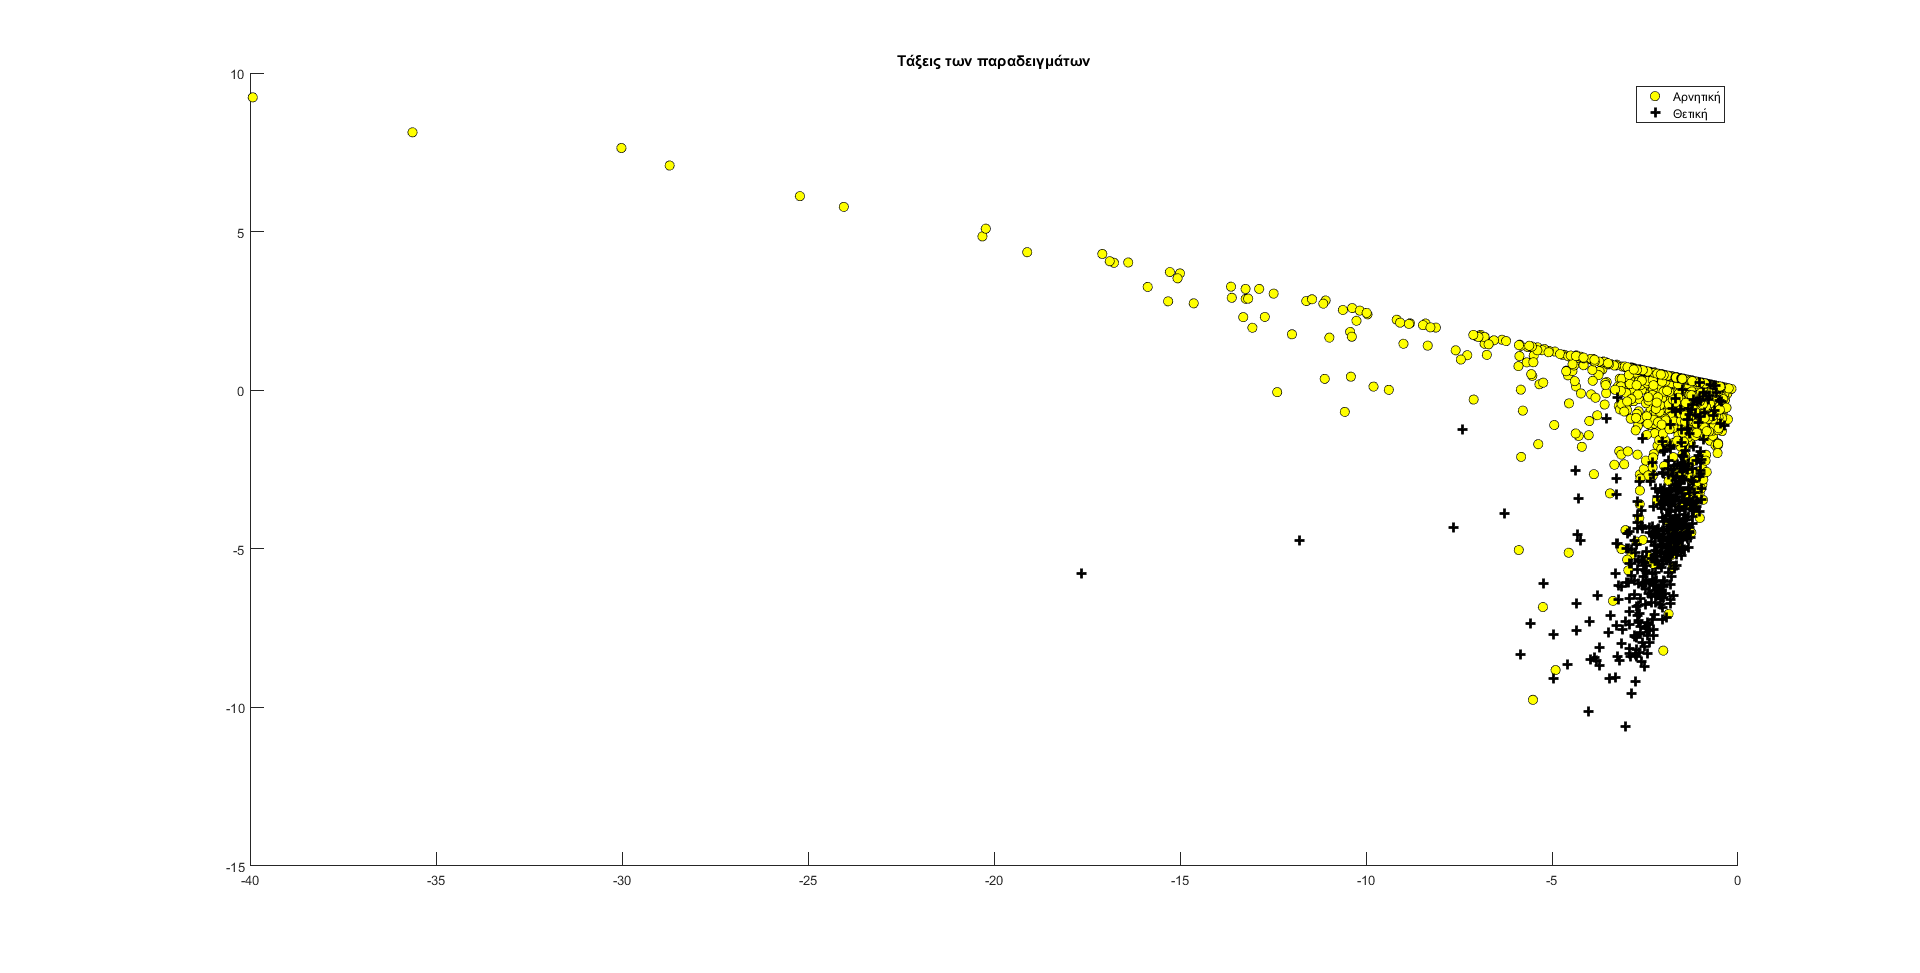
\includegraphics[width=160mm, height=100mm]{../../plots/gr_class_semi_sup.png}
\caption{Χαρακτηριστικά και τάξεις καταναλωτών}
\label{fig:charclasscons}
\end{figure}
\newpage
Στο Σχήμα \ref{fig:viewandthreshold} παρατηρούνται οι ισοϋψείς καμπύλες της Γκαουσιανής κατανομής. Το Σχήμα \ref{fig:threshanomalydetection1} εμφανίζει την προσαρμογή στα δεδομένα του τυπικού αλγορίθμου, ενώ το Σχήμα \ref{fig:threshanomalydetection2} αποδίδει την προσαρμογή στα δεδομένα του εναλλακτικού αλγορίθμου. Στην πρώτη περίπτωση, είναι εμφανές πως η οριοθέτηση της κατανομής γίνεται σε ένα στενό κύκλο, ενώ στη δεύτερη περίπτωση η οριοθέτηση γίνεται με πιο πλατή κύκλο. Λαμβάνοντας υπόψη τα παραπάνω, γίνεται για άλλη μια φορά σαφές πως η μείωση διαστάσεων δε βοηθά στη βελτιστοποίηση του αλγορίθμου άμεσα, αλλά δίνει μια άλλη οπτική των δεδομένων.\par
Η οριοθέτηση γίνεται μόνο στα δεδομένα δοκιμής που στον τυπικό αλγόριθμο είναι το 70\% των δεδομένων, ενώ στον εναλλακτικό αλγόριθμο είναι το 35\%. Παράλληλα, η υλοποίησή της έχει σαν είσοδο τον μέσο όρο της και τη διακύμανση που παρήχθησαν στη δημιουργία του μοντέλου. Η χάραξη των ισοϋψών καμπυλών γίνεται με τη βοήθεια ενός δισδιάστατου πλέγματος που ορίζεται παρατηρώντας τη διάταξη των δεδομένων στο επίπεδο. Εξάγοντας τις πιθανότητες της πολυμεταβλητής Γκαουσιανής κατανομής με είσοδο το πλέγμα και τον μέσο όρο και διακύμανση, δημιουργούνται 7 ομόκεντρα περιγράμματα. Η ακριβής οριοθέτηση ορίζεται από την διαδικασία βελτιστοποίησης του \en{F1 score}.\par
\clearpage
\begin{figure}[ht!]
\begin{subfigure}[b]{0.8\textwidth}
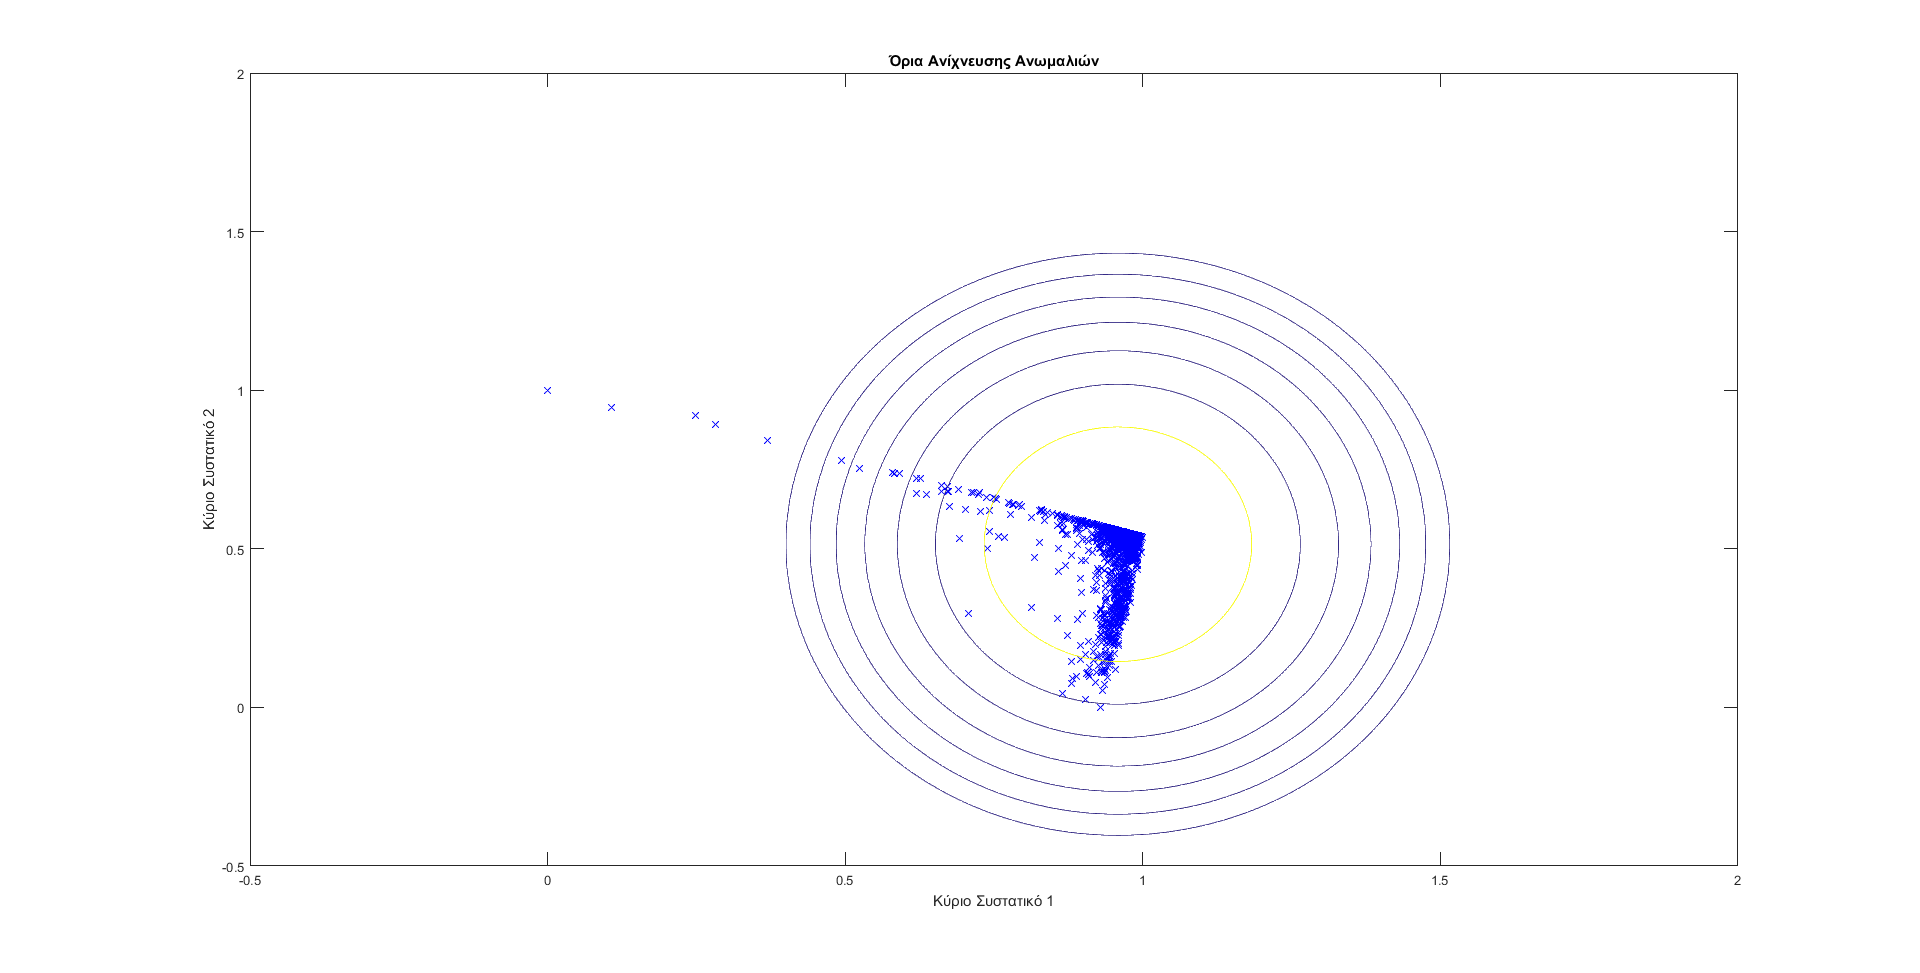
\includegraphics[width=160mm, height=100mm]{../../plots/gr_threshold_semi_sup_1.png}
\caption{Προσαρμογή κατανομής στα τυπικά δεδομένα}
\label{fig:threshanomalydetection1}
\end{subfigure}

\begin{subfigure}[b]{0.8\textwidth}
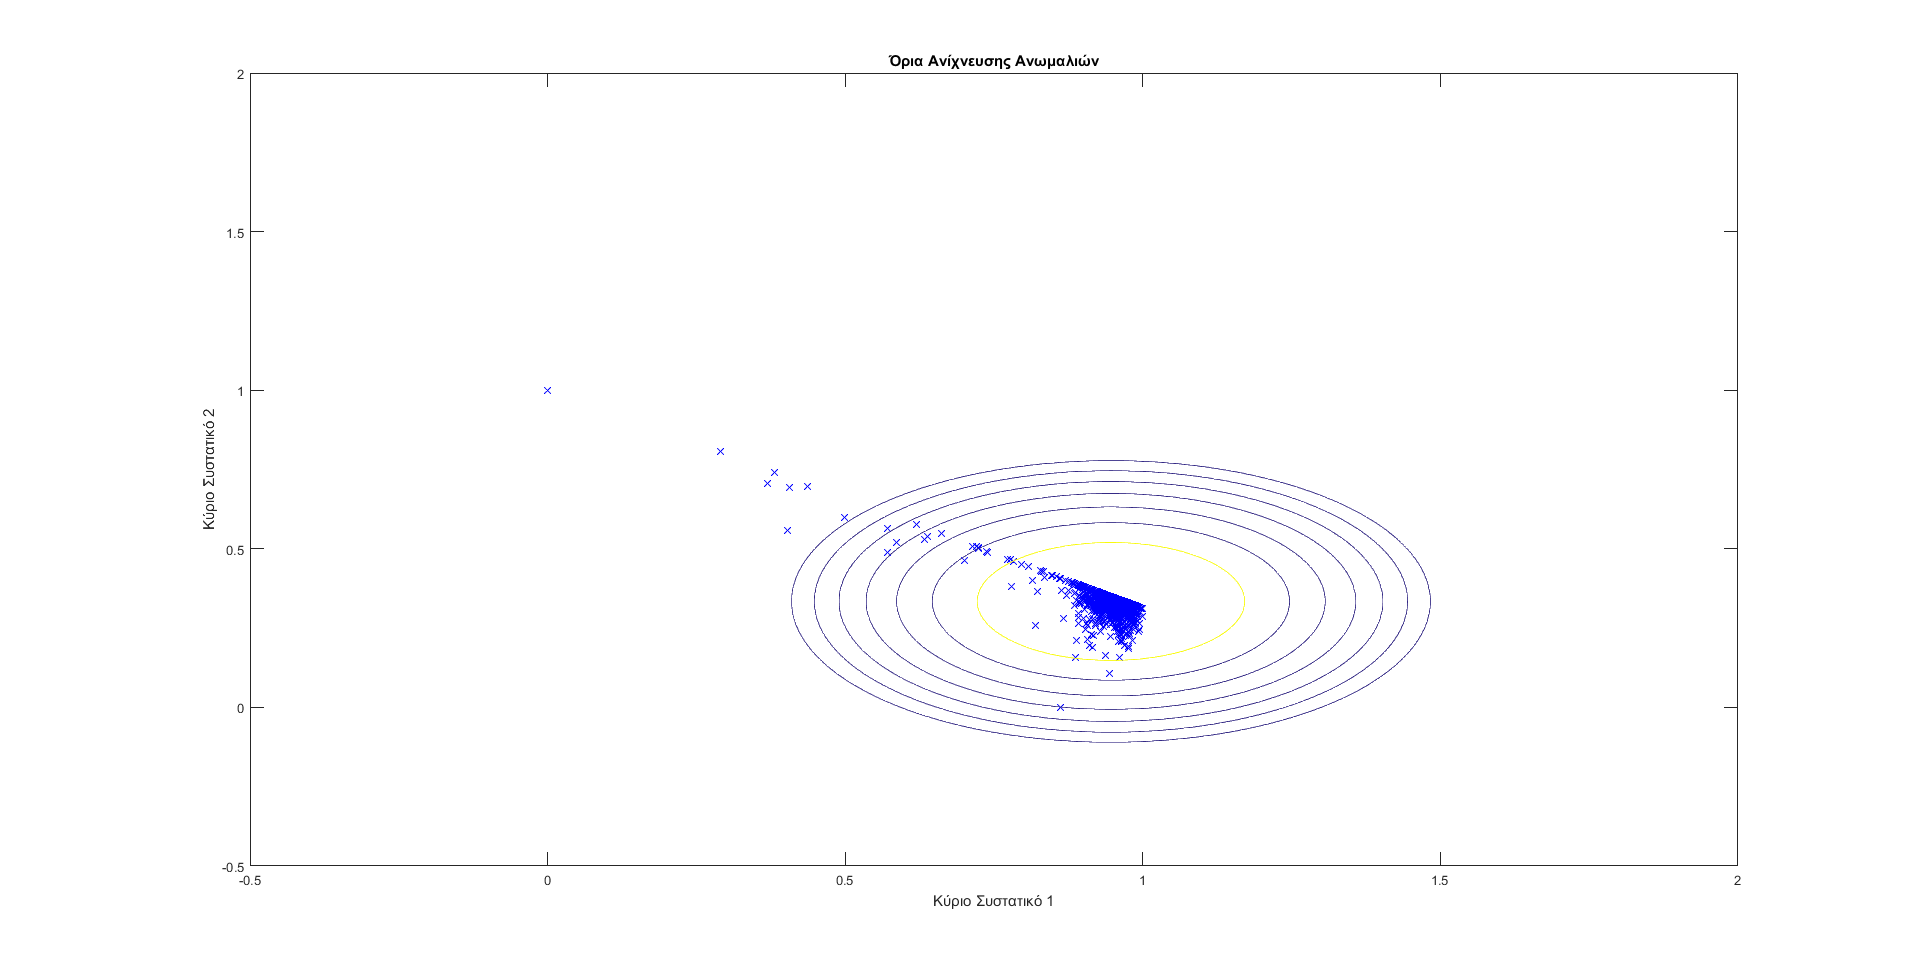
\includegraphics[width=160mm, height=100mm]{../../plots/gr_threshold_semi_sup_2.png}
\caption{Προσαρμογή κατανομής στα ενναλακτικά δεδομένα}
\label{fig:threshanomalydetection2}
\end{subfigure}

\caption{Ισοϋψείς Γκαουσιανής κατανομής}
\label{fig:viewandthreshold}
\end{figure}
\newpage
Για να αποδειχθεί και με αποτελέσματα η παραπάνω υπόθεση, γίνεται μια νέα σειρά δοκιμών με τον αλγόριθμο μείωσης διάστασης.
\begin{center}
\begin{longtabu} to 0.8\textwidth {| c | c || c | c | c | c | c |   }
 \hline
 Σύστημα & Πύλη &\en{DR}  & \en{FPR} & \en{Accuracy} & \en{F1 score} & \en{BDR \%}\\
\hline
τυπικό&\en{AND} & 79.01 & 2.51 & 95.59 & 78.65 & 78\\
 \hline
 εναλλακτικό& \en{AND}& 0.00 & 0.00  & 80.28 &  - &  -\\ 
\hline
εναλλακτικό& \en{OR}& 87.85 & 11.79  & 88.14 & 73.44 & 45\\ 
 \hline
\caption{Εξερεύνηση μείωσης διάστασης στους ημι-επιβλεπόμενους αλγορίθμους}
\label{tab:testpcasemisup}
\end{longtabu}
\end{center}

\subsection{Αποτελέσματα δοκιμής συστημάτων}
Για την τελική δοκιμή επιλέχθηκαν όλοι οι πιθανοί καταναλωτές και εισήχθη 10\% ποσοστό κλοπών. Ένας ικανοποιητικός τρόπος να παρατηρηθεί η λειτουργία του αλγορίθμου είναι να δοκιμαστεί το σύστημα υπό διαφορετικές εντάσεις κλοπής. Έτσι επιλέχθηκαν τα συστήματα με \en{K-Means}, χωρίς μείωση διάστασης και πύλες \en{AND} που είχαν τα πιο συνεπή αποτελέσματα.\par
Στον τυπικό αλγόριθμο παρατηρούνται ομαλές καμπύλες με συνεχή αύξουσα πορεία στο \en{DR} και σχεδόν συνεχή φθίνουσα στο \en{FPR}. Παράλληλα, αξίζει να σημειωθεί πως ενώ το \en{DR} δεν φτάνει το 100\% αλλά το 90\%, το \en{FPR} φτάνει σε εξαιρετικά χαμηλά επίπεδα πράγμα που ουσιαστικά σημαίνει ότι πρόκειται για ένα αρκετά συμπαγές και έμπιστο σύστημα.\par
Από την άλλη πλευρά, ο εναλλακτικός αλγόριθμος έχει και αυτός ομαλή καμπύλη \en{DR} με αύξουσα κυρίως πορεία, αλλά η καμπύλη \en{FPR} έχει ιδιαίτερα περίεργη συμπεριφορά. Το σύστημα φαίνεται πως όσο η ένταση αυξάνει τη σιγουριά της πρόβλεψης ως προς την απάτη, παράλληλα αυξάνει σε τόσο μεγάλο ποσοστό και την ενοχοποίηση των καταναλωτών, επιλέγοντας πιο αυθαίρετα τη θετική κλάση, με αποτέλεσμα τη σταδιακή αύξηση και των δύο μετρικών.
\begin{figure}[ht!]
\centering
\begin{subfigure}[b]{0.4\textwidth}
 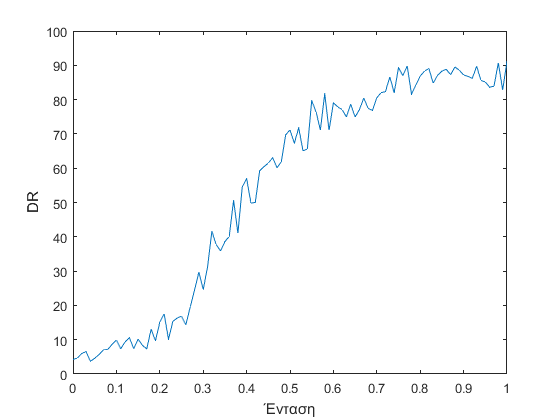
\includegraphics[width=70mm, height=50mm]{../../plots/gr_dr_intensity_semi_sup1.png}
\caption{\en{DR} συναρτήσει της έντασης του τυπικού αλγορίθμου}
\label{fig:testintdrsemisup1}
\end{subfigure}
\quad
\begin{subfigure}[b]{0.4\textwidth}
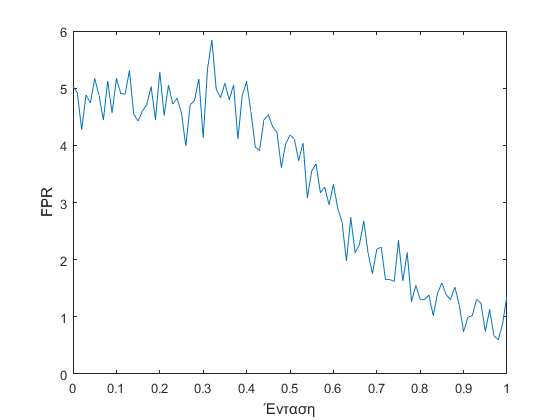
\includegraphics[width=70mm, height=50mm]{../../plots/gr_fpr_intensity_semi_sup1.png}
\caption{\en{FPR} συναρτήσει της έντασης του τυπικού αλγορίθμου}
\label{fig:testintfprsemisup1}
\end{subfigure}
\quad
\begin{subfigure}[b]{0.4\textwidth}
 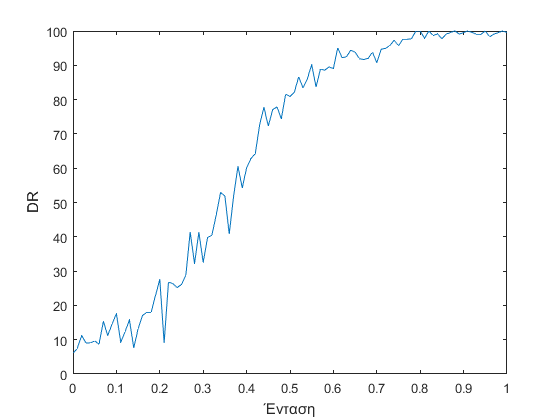
\includegraphics[width=70mm, height=50mm]{../../plots/gr_dr_intensity_semi_sup2.png}
\caption{\en{DR} συναρτήσει της έντασης του εναλλακτικού αλγορίθμου}
\label{fig:testintdrsemisup2}
\end{subfigure}
\quad
\begin{subfigure}[b]{0.4\textwidth}
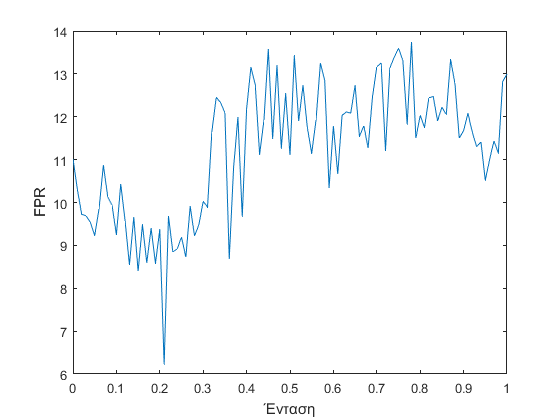
\includegraphics[width=70mm, height=50mm]{../../plots/gr_fpr_intensity_semi_sup2.png}
\caption{\en{FPR} συναρτήσει της έντασης του εναλλακτικού αλγορίθμου}
\label{fig:testintfprsemisup2}
\end{subfigure}

\caption{Δοκιμή έντασης ημι-επιβλεπόμενων συστημάτων}
\label{fig:testintensitysemisup}
\end{figure}
\newpage
\section{Σχόλια}
Στο παρόν κεφάλαιο έγινε μια διεξοδική αναζήτηση μη επιβλεπόμενων και ημι-επιβλεπόμενων συστημάτων με σκοπό την άμεση σύγκριση με τον αλγόριθμο επιβλεπόμενης μάθησης. Τα αποτελέσματα δείχνουν πως μπορεί να υπάρξει σύστημα που εντοπίζει μη τεχνικές απώλειες χωρίς καμία εκπαίδευση και χωρίς τη χρήση δυαδικών χαρακτηριστικών. Παράλληλα, η επίδοση του ημι-επιβλεπόμενου συστήματος δίνει τη δυνατότητα κατανόησης πως ακόμη και με λίγα δυαδικά χαρακτηριστικά ο μη επιβλεπόμενος αλγόριθμος μπορεί να γίνει πιο αξιόπιστος στην αναγνώριση απάτης και να βελτιώσει την επίδοσή του. Συγκρίνοντας τους ημι-επιβλεπόμενους αλγόριθμους, γίνεται φανερό πως η τυπική ανίχνευση ανωμαλιών είναι γενικά πιο προβλέψιμη και πιο εύστοχη.\par
Συνοψίζοντας, καθίσταται σαφές πως οι δύο συνιστώσες ταξινόμησης είναι απαραίτητες για την εξαγωγή ικανοποιητικών μετρικών και πως η αλληλεπίδρασή τους καθιστά την ταξινόμηση αξιόπιστη. Από την άλλη πλευρά,  η μέθοδος συσταδοποίησης δεν έχει εξαιρετική σημασία για την απόδοση του συστήματος, ακόμη και όταν αλλάζει η μέθοδος και στους δύο άξονες ταξινόμησης. Τέλος, για την αύξηση εμπιστοσύνης στα συστήματα απαιτείται η χρήση της πύλης \en{AND} για την τελική δυαδική πράξη των ταξινομητών, καθώς επιτυγχάνει ικανοποιητικά αποτελέσματα σε δύο πολύ σημαντικές μετρικές, το \en{F1 score} και το \en{Accuracy}.


\chapter{Δυσκολίες στην εκπόνηση της διπλωματικής}
Στην παρούσα διπλωματική αντιμετωπίστηκαν δυσκολίες που εν μέρει όρισαν την μελλοντική πορεία του ζητήματος. Υπήρξαν δύο ειδών τεχνικές δυσκολίες στην ανίχνευση μη τεχνικών απωλειών σε ετήσια δεδομένα. Η πρώτη βασίζεται στο γεγονός ότι πρόκειται για ετήσιες χρονοσειρές που δεν μπορεί εύκολα να αποτυπωθεί μια αξιόπιστη καταναλωτική συμπεριφορά. Η δεύτερη στο γεγονός της ευρείας χρήσης και δοκιμής πολλών ταξινομητών αντιμετωπίζοντας τις ιδιαίτερες απαιτήσεις του καθενός. Παράλληλα, πρέπει να ορισθεί και ένα όριο στην αξιοπιστία των συστημάτων μηχανικής μάθησης, καθώς ένα αποτελεσματικό σύστημα πρέπει να έχει σιγουριά στον εντοπισμό του ζητούμενου συμβάντος και να ελαχιστοποιεί τα περιθώρια λάθους εκτίμησης.\par
Στην πιο ευρεία σφαίρα του ζητήματος τίθενται θέματα ιδιωτικότητας στους καταναλωτές, ενώ τους δίνεται η δυνατότητα ανωνυμοποίησης των δεδομένων τους \cite{anonymization} γεγονός που δυσκολεύει σε μεγάλο βαθμό την εξόρυξη δεδομένων σε επόμενα στάδια. Με την ύπαρξη των έξυπνων μετρητών ανοίγεται ένα παράθυρο που εκθέτει τις προσωπικές δραστηριότητες σε οποιονδήποτε έχει πρόσβαση σε καταναλωτικές πληροφορίες. Οι τεράστιες δυνατότητες που ανοίγονται στην αναλυτική μελέτη χρονοσειρών δεν θα μπορούσε να συμβαίνει χωρίς την αντιμετώπιση και του ανθρώπινου παράγοντα, καθώς πρόκειται για ατομικές καταναλώσεις.
\section{Τεχνικά εμπόδια}
Η αντιμετώπιση τεχνικών θεμάτων πάντα απαιτεί τη λεπτομερή ανάλυση της δυσκολίας και λήψεις αποφάσεων. Η έκταση των δεδομένων αποδείχθηκε σχετικά μικρή, καθώς τα συστήματα δεν είχαν τη δυνατότητα παρατήρησης των καταναλωτικών συνηθειών σε μεγάλο βάθος χρόνου. Το συγκεκριμένο πρόβλημα γεννά νέες δυσκολίες και μπορεί να εγείρει την αναξιοπιστία του συστήματος σε δεδομένα άλλων χρονικών περιόδων. Τέλος, αξίζει να ληφθεί υπόψη πως η διαδικασία εύρεσης και επεξεργασίας δεδομένων και χαρακτηρισμών τους είναι εξαιρετικά επίπονη και απαιτεί εμπιστοσύνη στην πηγή τους. 
\subsection{Έλλειψη μακροχρόνιων δεδομένων}
Για να μπορέσει να αντιμετωπιστεί το ζήτημα των μη-τεχνικών απωλειών με μακροπρόθεσμο ορίζοντα απαιτείται η βαθιά κατανόηση της συχνότητας των προτύπων και των στιγμιότυπων των χρονοσειρών. Με αυτό τον τρόπο αναλύονται σε βάθος οι καταναλωτικές συνήθειες και γνωστοποιούνται οι μεταβλητές που τις επηρεάζουν. Τα δεδομένα της παρούσας εργασίας αφορούσαν χρονικό διάστημα που δεν ξεπερνούσε τα δύο έτη. Με τέτοιο εύρος μετρήσεων ήταν λοιπόν λογικό να περιοριστούν οι δοκιμές σε ετήσιες.\par
Εκεί που εγείρεται η σημαντική δυσκολία είναι το γεγονός ότι οι καταναλωτές ταξινομούνται με ένα και μόνο έτος αναφοράς στο αν εμφανίζεται ύποπτο προφίλ κατανάλωσης. Ειδικότερα ο αλγόριθμος χρησιμοποιεί τις γενικές καταναλωτικές συνήθειες του έτους για να ταξινομήσει κάθε καταναλωτή με αυτά τα κριτήρια. Η πιο ασφαλής προσέγγιση θα απαιτούσε να υπάρχει μεγάλο χρονικό παράθυρο κατανάλωσης για να κριθεί ένα έτος ύποπτο, για να μπορεί εύκολα κάποιος να παρατηρήσει μια ασυνήθιστη τάση των δεδομένων. Έτσι θα μπορούσαν να οργανωθούν ευκολότερα οι καταναλωτές σε ομάδες που θα είχαν μια γενικότερη ομοιότητα ως προς τις καταναλωτικές συνήθειες.
\subsection{Έλλειψη παραδειγμάτων}
Παράλληλα, έχει νόημα να παρατηρηθεί πως το δείγμα των καταναλωτών δεν είναι τελείως αντιπροσωπευτικό για την γενίκευση σε ένα μεγαλύτερο πληθυσμό. Ειδικότερα, οι 4.500 καταναλωτές θα μπορούσαν να είχαν πολύ διαφορετικές συνήθειες αν ζούσαν σε διαφορετική τοποθεσία, άρα και διαφορετικές χρονοσειρές που θα εξετάζονταν διαφορετικά αν απέκλιναν σημαντικά από τις υπάρχουσες. Το πρόβλημα εντείνεται παρακολουθώντας την ομοιογένεια των τύπων των καταναλωτών. Εμφανίζεται μια κυρίαρχη ομάδα που έχει σχετική ομοιογένεια μεταξύ της και αποτελείται από νοικοκυριά και οικιακούς χρήστες. Στην ομάδα αυτή ανήκουν τουλάχιστον τα τρία τέταρτα του δείγματος κάτι που έχει εκμεταλλευτεί από τα συστήματα ταξινόμησης, αλλά αίρει ερωτήματα για το υπόλοιπο ένα τέταρτο του πληθυσμού. Το υπόλοιπο ένα τέταρτο στελεχώνεται από καταναλωτές με υψηλές ενεργειακές απαιτήσεις, δηλαδή από μικρο-μεσαίες επιχειρήσεις. Αυτό το μικρό δείγμα δεν μπορεί να εξάγει εύκολα μια γενικευμένη συμπεριφορά που να εκφράζει όλο το σύνολο, καθώς κάθε επιχείρηση ανάλογα με τις ανάγκες της προσαρμόζει τη λειτουργία της. Αποτέλεσμα είναι να έχουμε ένα ικανοποιητικό πλήθος ομοιόμορφων καταναλωτών που εξάγουν όμοια χαρακτηριστικά και ένα μικρό υποσύνολο των δεδομένων με επιχειρήσεις που έχουν μεγάλες και αδιευκρίνιστες ανάγκες.
\subsection{Δυσκολία επιλογής μετρικών}
Στην παρούσα διπλωματική χρησιμοποιήθηκε πλήθος αλγορίθμων μηχανικής μάθησης με κάθε ένα να έχει τα δικά του ιδιαίτερα χαρακτηριστικά. Δημιουργήθηκε λοιπόν η ανάγκη σύγκρισης των αλγορίθμων βάση κάποιων απόλυτων μετρικών για την τελική αξιολόγησή τους. Ειδικότερα, οι επιβλεπόμενοι αλγόριθμοι χρησιμοποιούν 70\% των δεδομένων για εκπαίδευση και το 30\% για προβλέψεις, οι μη-επιβλεπόμενοι αλγόριθμοι δεν χρησιμοποιούν εκπαίδευση για τη δημιουργία μοντέλου πρόβλεψης, ενώ οι ημι-επιβλεπόμενοι αλγόριθμοι χρησιμοποιούν 70\% για την εξαγωγή του στατιστικού μοντέλου και την πρόβλεψη και 30\% για τη βελτιστοποίηση του μοντέλου. Όπως γίνεται αντιληπτό οι προβλέψεις γίνονται σε διαφορετικά δείγματα των πληθυσμών δημιουργώντας απαίτηση για αξιόπιστες μετρικές.\par
Τα \en{DR} και \en{FPR} μπορούν γρήγορα να δώσουν μια πρώτη αίσθηση για την ευστοχία του αλγορίθμου, αλλά λόγο της ευαισθησίας του προβλήματος δεν πρέπει να θεωρούνται οι κύριες μετρικές. Αυτό οφείλεται στο γεγονός ότι ένας αλγόριθμος με πολύ υψηλό \en{DR} μπορεί να αναγνωρίσει τις κλοπές, αλλά αν έχει \en{FPR} που ξεπερνά το 5\% οι προβλέψεις δεν θεωρούνται εντελώς αξιόπιστες, καθώς εισάγεται μεγάλο περιθώριο λάθους. Ένας τρόπος να αποτυπωθεί η σχέση μεταξύ του \en{DR} και \en{FPR} είναι το \en{F1 score}, που έχει εξάρτηση και από τις δύο μετρικές και εξάγει ικανοποιητικά αποτελέσματα μόνο με χαμηλό \en{FPR}. Παράλληλα, ένας γενικότερος τρόπος να εξεταστεί η ταξινόμηση είναι με την ευστοχία \en{Accuracy} που πρέπει να βρίσκεται πάντα πάνω από το 90\% και περιγράφει την γενικότερη πρόβλεψη του συστήματος. Όταν οι αλγόριθμοι έχουν παρόμοιες αυτές τις μετρικές αξίζει να ελεγχθεί το \en{BDR} που προσφέρει μια πιθανοτική προσέγγιση. Ειδικότερα ορίζει την πιθανότητα να είναι κλοπή δεδομένου ότι προβλέφθηκε απάτη.
\subsection{Εύρεση αξιόπιστων δυαδικών χαρακτηρισμών}
Ένα σημαντικός παράγοντας που δεν πρέπει να αμεληθεί είναι η αξιοπιστία και η προέλευση των δυαδικών χαρακτηριστικών των χρονοσειρών. Στην παρούσα εργασία δεν απαιτήθηκε να ευρεθούν τέτοια δεδομένα, καθώς προσομοιώθηκαν οι απάτες. Στην περίπτωση όμως που τα δεδομένα έρχονται με δυαδικούς χαρακτηρισμούς από ένα φορέα, απαιτείται έλεγχος στη μεθοδολογία εξαγωγής των χαρακτηριστικών. Η εγκυρότητα των δυαδικών αυτών διανυσμάτων είναι καίριας σημασίας για την εκπαίδευση και έλεγχο του συστήματος, καθώς είναι η βάση της υλοποίησης των αλγορίθμων και αποτελούν την κινητήριο δύναμη των αλγορίθμων βελτιστοποίησης. Επιπρόσθετα αξίζει να σημειωθεί πως θα μπορούσε να δημιουργηθεί ένα σύστημα με ανατροφοδότηση των φυσικών ελέγχων για τη δημιουργία αξιόπιστων δυαδικών χαρακτηριστικών.\par
\section{Ασφάλεια Καταναλωτών}
Η εισαγωγή των έξυπνων μετρητών στην καθημερινότητά μας δίνει τη δυνατότητα να διερευνηθούν σε βάθος οι καταναλώσεις ενέργειας και διευκολύνει την επικοινωνία των δεδομένων με εγκεκριμένους φορείς. Αυτή όμως η πραγματικότητα έχει και μια σκοτεινή πτυχή που αντιμετωπίζεται στις περισσότερες μελέτες μεγάλης κλίμακας δεδομένων. Οι πληροφορίες των πελατών είναι εκτεθειμένες σε ένα δίκτυο αμφίδρομης επικοινωνίας καταναλωτών και πάροχων, ενώ ανά πάσα στιγμή κάποιος εργαζόμενος μπορεί να ανατρέξει σε αυτές για προσωπικούς λόγους.\par
Η σημερινή τεχνολογία των έξυπνων μετρητών βασιζόμενων στο \en{NALM} αλγόριθμο, παρέχει τρόπους να αναγνωρίζονται συσκευές σε λειτουργία ακόμη και όταν πολλά νοικοκυριά συνυπολογίζονται. Έτσι, κάποιος κακόβουλος χρήστης θα μπορούσε να αντλήσει δεδομένα για το πρόγραμμα των νοικοκυριών, τα είδη των συσκευών τους και τις ανάγκες τους. Ένας τρόπος να αντιμετωπιστεί αυτό το θέμα είναι η διαχείριση της ενεργειακής χρήσης μέσα στο σπίτι, πριν συλλεχθούν τα δεδομένα του μετρητή.\par
Γίνεται λοιπόν σαφές πως οι έξυπνοι μετρητές χωρίς κάποιο σύστημα ανωνυμοποίησης είναι πλήγμα στην ιδιωτικότητα των καταναλωτών και αίρουν θέματα ασφαλείας. Η έρευνα σε αυτή την κατεύθυνση ξεπερνά αυτή τη διπλωματική εργασία, αλλά ήδη προτείνονται νέοι αλγόριθμοι και δικτυακές δομές για να μπορέσει να συμβαδίσει η ιδιωτικότητα με την αποτελεσματικότητα.



\chapter{Συμπεράσματα και δυνατότητες μελλοντικής επέκτασης}
Το κεφάλαιο αυτό συνοψίζει όλη τα γνώση που δημιουργήθηκε από τη μελέτη των αλγορίθμων και την εξαγωγή αποτελεσμάτων. Παράλληλα, κάνοντας ένα βήμα πίσω δημιουργείται άλλη οπτική στην αντιμετώπιση του θέματος του εντοπισμού των μη-τεχνικών απωλειών. Παρατηρούνται τα πλεονεκτήματα και τα μειονεκτήματα κάθε συστήματος δίνοντας βάση στο εύρος του πεδίου εφαρμογής του καθενός και στις δυνατότητές του. Τέλος γίνονται κάποιες επισημάνσεις που αφορούν έχουν ως κύριο μέλημα τη βελτιστοποίηση των συστημάτων.
\section{Σύγκριση αποτελεσμάτων}
Κάνοντας μια επισκόπηση στα αποτελέσματα εύκολα παρατηρείται πως ο επιβλεπόμενος αλγόριθμος έχει την καλύτερη σχέση μεταξύ ποσοστού ευστοχίας στην εύρεση \en{DR} και ποσοστού λάθος προβλέψεων \en{FPR}. Αυτό ήταν αναμενόμενο από τα πρώτα στάδια της διπλωματικής, καθώς ο επιβλεπόμενος αλγόριθμος είναι ευρέως μελετημένος και είναι κοινή γνώση η αποτελεσματικότητά του σε τέτοιου είδους δεδομένα. Παράλληλα, παρατηρείται πως ο αλγόριθμος μη-επιβλεπόμενης μάθησης έχει υψηλότερο \en{DR}, αλλά και υψηλότερο \en{FPR} που είναι στα όρια της κόκκινης γραμμής που ορίστηκε στο 5\%. Με αυτό το σκεπτικό δημιουργήθηκε το ημι-επιβλεπόμενο σύστημα, ώστε να χαμηλώσει το \en{FPR} και να έχουμε πιο σίγουρες προβλέψεις.\par
Τίθεται, λοιπόν σαν άξονας αναφοράς ο επιβλεπόμενος αλγόριθμος που από τη μία έχει τα καλύτερα αποτελέσματα από τους αλγορίθμους, αλλά από την άλλη είναι ο λιγότερο εφαρμόσιμος σε πραγματικά προβλήματα, λόγω της ανάγκης ύπαρξης δυαδικών χαρακτηριστικών. Συγκρίνοντας τα συστήματα με τον επιβλεπόμενο αλγόριθμο παρατηρούνται τα εξής:
\begin{itemize}
\item Το μη επιβλεπόμενο σύστημα κατέχει το σημαντικότερο πλεονέκτημα που είναι η ευρεία και άμεση εφαρμογή του σε υπάρχοντα προβλήματα. Αυτό συμβαίνει, καθώς δεν απαιτεί κανενός είδους εκπαίδευσης, αλλά μόνο εφαρμογή συμπαγών και αξιόπιστων κανόνων που να διαχωρίζουν τις δύο κλάσεις. Παράλληλα, λόγο της έλλειψης εκπαίδευσης η δημιουργία του μοντέλου διαχωρισμού γίνεται ταχύτατα. Στα μειονεκτήματα του αλγορίθμου είναι η οριακή του γενική απόδοση. Το \en{FPR} είναι ακριβώς στα όρια ανοχής που ορίστηκαν (5\%), ενώ το \en{Accuracy} είναι λίγο χαμηλότερα από τα επιθυμητά επίπεδα (95\%).
\item Το ημι-επιβλεπόμενο σύστημα απαιτεί μόνο μικρό ποσοστό καταναλωτών για βελτιστοποίηση του ορίου επιλογής, γεγονός που το κάνει πιο εύκολα εφαρμόσιμο από το επιβλεπόμενο σύστημα, αλλά λιγότερο από το μη-επιβλεπόμενο σύστημα. Ουσιαστικά ο ημι-επιβλεπόμενος αλγόριθμος λειτουργεί σαν ενδιάμεση λύση σε όλα τα κριτήρια που έχουν τεθεί. Ειδικότερα η απόδοση του είναι βελτιωμένη με εξαιρετικά χαμηλό \en{FPR} και βελτιωμένο \en{Accuracy}. Παρόλο, που το σύστημα φαίνεται να έχει σχετικά χαμηλό \en{DR}, αυτό εξισορροπείται από τη σιγουριά της πρόβλεψης που δίνεται από το \en{BDR}. Πιο συγκεκριμένα το σύστημα όταν προβλέπει απάτη είναι 80\% σίγουρο ότι πρόκειται για απάτη, ποσοστό που προσεγγίζει σε μεγάλο βαθμό το επιβλεπόμενο σύστημα.
\end{itemize}

\begin{center}
\begin{longtabu}  to 0.8\textwidth { | c || c | c | c | c | c |  }
 \hline
Σύστημα & \en{DR}  & \en{FPR} & \en{Accuracy} & \en{F1} &  \en{BDR} \\
 \hline
επιβλεπόμενο & 80.87 & 1.54 & 96.96 & 81.94 & 0.85 \\
μη-επιβλεπόμενο & 86.44	& 5.43 & 93.76 & 73.47 & 0.64\\
ημί-επιβλεπόμενο & 71.09 & 2.00 & 95.49 & 74.64 & 0.80\\
\hline
\caption{Σύγκριση συστημάτων}
\label{tab:comparesystems}
\end{longtabu}
\end{center}

Για την οπτικοποίηση αυτών των παρατηρήσεων δημιουργήθηκε ένα γράφημα δίνοντας βάση στο \en{Accuracy}, \en{F1 score} και \en{BDR}. Καθίσταται λοιπόν σαφές πως η ημι-επιβλεπόμενη μάθηση βρίσκεται ακριβώς ανάμεσα στις επιδόσεις και στη χρηστικότητα του επιβλεπόμενου και μη-επιβλεπόμενου συστήματος.

\begin{figure}[ht!]
\centering
 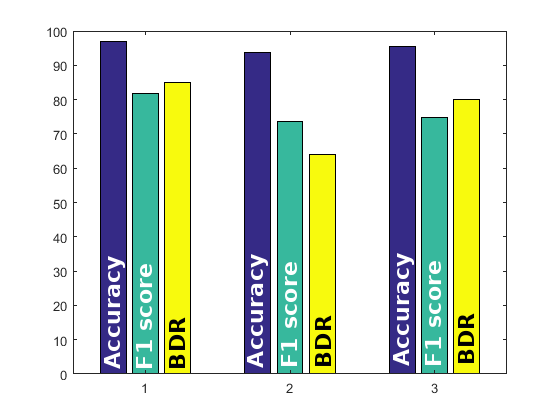
\includegraphics[width=90mm, height=60mm]{../../plots/comparison_systems.png}
 \caption{Σύγκριση συστημάτων}
\label{fig:comparisonsystem}
 \end{figure}
\section{Συμπερασματικές σημειώσεις}
Συνοψίζοντας χρήσιμες πληροφορίες που παρήχθησαν από αυτή τη μελέτη γίνεται σαφές πως η ανίχνευση μη-τεχνικών απωλειών με αλγορίθμους και συστήματα μηχανικής μάθησης είναι εφικτή και μάλιστα και με υποσχόμενα αποτελέσματα. Οι γραμμικοί ταξινομητές μπορούν με μεγάλη επιτυχία να εντοπίσουν με ένα έτος  εκπαίδευσης αν έχει εγκατασταθεί σύστημα αλλοίωσης των μετρήσεων. Η συσταδοποίηση των κανονικοποιημένων χρονοσειρών έχει επίσης πολύ καλά αποτελέσματα στον διαχωρισμό του κυρίως πληθυσμού με μικρότερα δείγματα ασυνήθιστων μετρήσεων. Το γεγονός αυτό είναι και ο λόγος που αποτέλεσε το βασικό συστατικό του μη-επιβλεπόμενου και ημί-επιβλεπόμενου συστήματος. Χρησιμοποιήθηκαν δύο ειδών κανονικοποιήσεις παρατηρώντας πως η κανονικοποίηση σε εύρος [-1,1] ταιριάζει στις χρονοσειρές, ενώ σε εύρος [0,1] σε χαρακτηριστικά διαχωρισμού  με αραιούς πίνακες. Τέλος, καθίσταται σαφές πως η σύνδεση και αλληλεπίδραση διαφορετικών αλγορίθμων για τη δημιουργία μιας τελικής ταξινόμησης μπορεί να λειτουργήσει ικανοποιητικά παρόλο που έχει τεράστια περιθώρια δοκιμών και βελτιστοποιήσεων.
\section{Μελλοντική επέκταση}
Καταλήγοντας στην παρούσα διπλωματική αναλύθηκε ευρύ φάσμα αλγορίθμων μηχανικής μάθησης με επιτυχία, αλλά το ταξίδι για την βελτιστοποίηση συστημάτων μηχανικής μάθησης δεν έχει τέλος. Έτσι, σε αυτό το σημείο αξίζει να αναφερθούν οι μελλοντικές επεκτάσεις που πιστεύεται πως θα μπορούσαν να εξάγουν όμοια ή και καλύτερα αποτελέσματα στο πρόβλημα της ταξινόμησης. Πιο συγκεκριμένα τα συστήματα που δημιουργήθηκαν θα μπορούσαν να συμπεριλάβουν τα εξής:
\begin{itemize}
\item Εφαρμογή ταξινόμησης σε περισσότερες από δύο κλάσεις. Όλα οι ταξινομήσεις που δοκιμάστηκαν σε αυτή τη διπλωματική έγιναν σε δύο κλάσεις, την αρνητική και την θετική. Παρόλα αυτά τα αποτελέσματα έδειξαν ότι υπάρχουν καταναλωτές με ακανόνιστες χρονοσειρές που δεν έχουν ομοιότητες ούτε με τις πραγματικές χρονοσειρές (αρνητική κλάση), αλλά ούτε και με τις προσομοιομένες (θετική κλάση). Για αυτό το λόγο θα είχε νόημα δημιουργηθούν και άλλες κλάσεις που να ενδεικνύουν ιδιαίτερη καταναλωτική συμπεριφορά, αλλά όχι ρευματοκλοπή. Έτσι θα καθιστόταν εφική η περαιτέρω μείωση των λάθος προβλέψεων.
\item Εξερεύνηση τεχνικών ανίχνευσης ανωμαλιών. Στην ανίχνευση ανωμαλιών στον ημι-επιβλεπόμενο αλγόριθμο χρησιμοποιήθηκε παραμετρική τεχνική Γκαουσιανού μοντέλου, καθώς είναι η συνηθέστερη τεχνική. Παρ' όλα αυτά υπάρχουν ενδείξεις από τους γραμμικούς ταξινομητές πως οι παλινδρομήσεις των χρονοσειρών οδηγούν σε αξιόλογα αποτελέσματα. Θα είχε λοιπόν νόημα να δοκιμαστεί ανίχνευση ανωμαλιών βάσει του μοντέλου παλινδρόμησης. Παράλληλα, θα είχε ενδιαφέρον η προσέγγιση του αλγορίθμου από τη μη παραμετρική σκοπιά βάσει των ιστογραμμάτων και των συναρτήσεων πυρήνων, καθώς ήδη στην παρούσα διπλωματική υπάρχουν ενδείξεις με υποσχόμενα αποτελέσματα στο κεφάλαιο \ref{sec:histograms} κκαι \ref{sec:RBFkernel} αντίστοιχα.
\item Ταξινόμηση βάσει πρόβλεψης μελλοντικής χρονοσειράς. Δεδομένης ύπαρξης δεδομένων με μεγαλύτερο χρονικό ορίζοντα θα καθιστόταν δυνατή η καλύτερη κατανόηση των μεταβλητών που επηρεάζουν το επίπεδο της κατανάλωσης. Με αυτό τον τρόπο θα μπορούσε κάθε καταναλωτής να αποκτά μια πρόβλεψη της κατανάλωσης του για το επόμενο έτος με μικρή απόκλιση από την πραγματική του κατανάλωση. Στην περίπτωση που η πρόβλεψη απέκλινε σημαντικά από την καταγραφείσα κατανάλωση ο καταναλωτής θα θεωρούνταν ύποπτος. Η προσέγγιση αυτή θεωρείται υποσχόμενη, καθώς η στατιστική μελέτη που έγινε στο κεφάλαιο \ref{sec:statisticalexplore}.
\end{itemize} 
%-----------------%


%OPTION #1: Embed bibliography from file `references.tex' using plain references.
%
\begin{thebibliography}{1}

\addcontentsline{toc}{chapter}{Βιβλιογραφία}

\bibitem{[ACC+03]} {\textlatin{
D.~J. Abadi, D.~Carney, U.~{\c{C}}etintemel, M.~Cherniack, C.~Convey, S.~Lee,  M.~Stonebraker, N.~Tatbul, and S.~Zdonik. 
Aurora: a new model and architecture for data stream management.
{\em The VLDB Journal -- The International Journal on Very Large Data Bases}, 12(2):120--139, 2003}}.

\bibitem{[DRS09]} {\textlatin{
N.~Dalvi, C.~R{\'e}, and D.~Suciu. Probabilistic databases: Diamonds in the dirt. {\em Communications of the ACM}, 52(7):86--94, July 2009}}.

\bibitem{[GBE+00]} {\textlatin{
R.~H. G{\"u}ting, M.~H. B{\"o}hlen, M.~Erwig, C.~S. Jensen, N.~A. Lorentzos,
  M.~Schneider, and M.~Vazirgiannis.
A foundation for representing and querying moving objects.
{\em ACM Transactions on Database Systems (TODS)}, 25(1):1--42, 2000}}.

\bibitem{[JMS+08]} {\textlatin{
N.~Jain, S.~Mishra, A.~Srinivasan, J.~Gehrke, J.~Widom, H.~Balakrishnan,
  U.~{\c{C}}etintemel, M.~Cherniack, R.~Tibbetts, and S.~Zdonik.
Towards a streaming {SQL} standard.
In {\em Proceedings of the VLDB Endowment}, 1(2):1379--1390, 2008}}.

\bibitem{[MHP05]} {\textlatin{
K.~Mouratidis, D.~Papadias, and M.~Hadjieleftheriou. 
Conceptual partitioning: an efficient method for continuous nearest
  neighbor monitoring.
In {\em Proceedings of the 24th ACM SIGMOD International
  Conference on Management of Data}, pages 634--645, 2005}}.

\bibitem{[Ora11]} {\textlatin{
{Oracle, Inc}.
Complex event processing {CQL} language reference.
\url{http://docs.oracle.com/cd/E16764_01/doc.1111/e12048/intro.htm }
  2009. Last accessed on 15/09/2013}}.

\bibitem{[PS11]} {\textlatin{
K.~Patroumpas and T.~Sellis.
Subsuming multiple sliding windows for shared stream computation.
In {\em Advances in
  Databases and Information Systems}, volume 6909 of Springer {\em Lecture Notes in
  Computer Science}, pages 56--69, 2011}}.

\bibitem{[RSV02]} {\textlatin{
P.~Rigaux, M.~Scholl, and A.~Voisard.
{\em Spatial databases: with application to {GIS}}.
Morgan Kaufmann, 2001}}.

\bibitem{[Pap15]}
Σεραφείμ Παπαδιάς.
Απόρριψη φόρτου από ρεύματα
  τροχιάς κινούμενων αντικειμένων. Διπλωματική Εργασία {\textlatin{\em DIPL-2015-02}} στο
Εργαστήριο Συστημάτων Βάσεων Γνώσεων και Δεδομένων, Εθνικό Μετσόβιο
  Πολυτεχνείο, Ιούλιος 2015.

\end{thebibliography}
%\addcontentsline{toc}{chapter}{Βιβλιογραφία}

%OPTION #2: Alternatively, prepare properly formatted BibTeX entries in file `references.bib'. 
%After processing with BibTeX, a file `main.bbl' is automatically populated and it is actually used for producing references in the resulting pdf. 
%IMPORTANT: You must manually modify `main.bbl' by adding \selectlanguage{english} (TOP) and \selectlanguage{english} (BOTTOM) in order to correctly display Latin and Greek characters in the final text.
\nocite{*}
\bibliography{references}


\appendix
\chapter{Αναλυτικά αποτελέσματα γραμμικών ταξινομητών}
\begin{table}[ht!]
\centering
\begin{tabular}{ |c||c|c|c|c|c|  }
 \hline
 Συνδυασμός & \en{DR}  & \en{FPR} & \en{Accuracy} & \en{F1 score} & \en{BDR} \\
 \hline
1 & 94.66 & 35.93 & 67.04 & 35.79 & 0.23 \\
  \hline
2 & 93.89 & 34.62 & 68.15 & 36.39 & 0.23 \\
  \hline
3 &92.37 & 39.70 & 63.41 & 32.88 & 0.21 \\
  \hline
4 & 91.67 & 21.23 & 80.15 & 49.62 & 0.32\\
  \hline
5 & 93.13 & 34.21 & 68.44 & 36.42 & 0.23\\
 \hline
6 & 91.60 & 35.11 & 67.48 & 35.35 & 0.22 \\
 \hline
7 & 93.89 & 34.29 & 68.44 & 36.61 & 0.23\\
 \hline
8 & 94.66 & 35.93 & 67.04 & 35.79 & 0.23\\
 \hline
\end{tabular}
\caption{Αποτελέσματα δοκιμής τύπου 1 κανονικοποίηση [-1,1]}
\label{tab:exploreclassifiers1norm2}
\end{table}

\begin{table}[ht!]
\centering
\begin{tabular}{ |c||c|c|c|c|c|  }
 \hline
 Συνδυασμός & \en{DR}  & \en{FPR} & \en{Accuracy} & \en{F1 score} & \en{BDR} \\
 \hline
1 & 75.65 & 1.38 & 96.67 & 79.45 & 0.86 \\
  \hline
2 & 80.00 & 1.46 & 96.96 & 81.78 & 0.86 \\
  \hline
3 &80.00 & 1.46 & 96.96 & 81.78 & 0.86 \\
  \hline
4 & 80.87 & 1.54 & 96.96 & 81.94 & 0.85\\
  \hline
5 & 81.74 & 1.94 & 96.67 & 80.69 & 0.82\\
 \hline
6 & 77.39 & 1.54 & 96.67 & 79.82 & 0.85 \\
 \hline
7 & 65.22 & 1.62 & 95.56 & 71.43 & 0.82\\
 \hline
8 & 75.65 & 1.46 & 96.59 & 79.09 & 0.85\\
 \hline
\end{tabular}
\caption{Αποτελέσματα δοκιμής τύπου 1 κανονικοποίηση [0,1]}
\label{tab:exploreclassifiers1norm1}
\end{table}

\begin{table}
\centering
\begin{tabular}{ |c||c|c|c|c|c|  }
 \hline
 Συνδυασμός & \en{DR}  & \en{FPR} & \en{Accuracy} & \en{F1 score} & \en{BDR} \\
 \hline
1 & 4.65 & 0.82 & 90.15 & 8.28 & 0.39\\
  \hline
2 & 12.40 & 3.77 & 88.22 & 16.75 & 0.27 \\
  \hline
3 & 10.08 & 3.19 & 88.52 & 14.36 & 0.26\\
  \hline
4 & 9.30 & 2.87 & 88.74 & 13.64 & 0.26\\
  \hline
5 & 13.18 & 4.01 & 88.07 & 17.44 & 0.27\\
 \hline
6 & 8.53 & 3.44 & 88.15 & 12.09 & 0.22\\
 \hline
7 & 0.78 & 0.41 & 90.15 & 1.48 & 0.17\\
 \hline
8 & 4.65 & 0.82 & 90.15 & 8.28 & 0.39\\
 \hline
\end{tabular}
\caption{Αποτελέσματα δοκιμής τύπου 2 με κανονικοποίηση [0,1]}
\label{tab:exploreclassifiers2}
\end{table}

\begin{table}
\centering
\begin{tabular}{ |c||c|c|c|c|c|  }
 \hline
 Συνδυασμός & \en{DR}  & \en{FPR} & \en{Accuracy} & \en{F1 score} & \en{BDR} \\
 \hline
 1 & 2.05 & 0.83 & 88.67 & 3.77 & 0.21\\
  \hline
 2 & 9.59 & 2.82 & 87.70 & 14.43 & 0.27\\
  \hline
 3 & 8.22 & 2.66 & 87.70 & 12.63 & 0.25\\
  \hline
 4 & 8.22 & 2.33 & 88.00 & 12.90 & 0.28\\
  \hline
 5 & 10.27 & 3.16 & 87.48 & 15.08 & 0.26\\
 \hline
 6 & 8.90 & 2.41 & 88.00 & 13.83 & 0.29\\
 \hline
7& 0.68 & 0.50 & 88.81 & 1.31 & 0.13\\
 \hline
8 & 2.05 & 0.83 & 88.67 & 3.77 & 0.21\\
 \hline
\end{tabular}
\caption{Αποτελέσματα δοκιμής τύπου 3 με κανονικοποίηση [0,1]}
\label{tab:exploreclassifiers3}
\end{table}

\begin{table}
\centering
\begin{tabular}{ |c||c|c|c|c|c|  }
 \hline
 Συνδυασμός & \en{DR}  & \en{FPR} & \en{Accuracy} & \en{F1 score} & \en{BDR} \\
 \hline
1 & 1.55 & 0.74 & 89.93 & 2.86 & 0.19\\
  \hline
2 & 10.85 & 3.03 & 88.74 & 15.56 & 0.28\\
  \hline
3 & 10.08 & 3.03 & 88.67 & 14.53 & 0.27\\
  \hline
4 & 5.43 & 2.70 & 88.52 & 8.28 & 0.18\\
  \hline
5 & 13.18 & 3.69 & 88.37 & 17.80 & 0.28 \\
 \hline
6 & 8.53 & 2.87 & 88.67 & 12.57 & 0.25\\
 \hline
7 & 0.00 & 0.25 & 90.22 &  NaN & 0.00\\
 \hline
8 & 1.55 & 0.66 & 90.00 & 2.88 & 0.21\\
 \hline
\end{tabular}
\caption{Αποτελέσματα δοκιμής μικτών τύπων με κανονικοποίηση [0,1]}
\label{tab:exploreclassifiersmix}
\end{table}

\begin{table}
\centering
\begin{tabular}{ |c|c|c|c| }
\hline
μικρός & 3 & 2 & 1\\
\hline
89.9300  & 88.6700 &  90.1500 &  96.6700\\
\hline
   88.7400  &  87.7000 &  88.2200 &  96.9600\\
   \hline
   88.6700  & 87.7000 &  88.5200  & 96.9600\\
   \hline
   88.5200  & 88.0000 &  88.7400  & 96.9600\\
   \hline
   88.3700  & 87.4800 &  88.0700  & 96.6700\\
   \hline
   88.6700  & 88.0000 &  88.1500  & 96.6700\\
   \hline
   90.2200  & 88.8100 &  90.1500  & 96.5600\\
   \hline
   90.0000  & 88.6700 &  90.1500  & 96.5900\\
\hline   
   \end{tabular}
\caption{Πίνακας \en{Accuracy} }
\label{tab:accuracytypes}
\end{table}

\begin{table}
\centering
\begin{tabular}{ |c|c|c|c|  }
\hline
1 & 2 & 3 & μικτός\\
\hline

   80.7800   & 8.2800 &   3.7700 &   2.8600\\
   \hline
   81.2300   &16.7500 &  14.4300 &  15.5600\\
\hline   
   79.2500   &14.3600 &  12.6300 &  14.5300\\
\hline
   79.8500   &13.6400 &  12.9000 &   8.2800\\
\hline   
   80.3100   &17.4400 &  15.0800 & 17.8000\\
   \hline
   78.6300   &12.0900 &  13.8300 &  12.5700\\
\hline   
   78.9100   & 1.4800 &   1.3100 &        0\\
\hline   
   81.2300   & 8.2800 &   3.7700 &   2.8800\\
\hline   
   \end{tabular}
\caption{Πίνακας \en{F1 score} }
\label{tab:F1scoretypes}
\end{table}
%\chapter{Τεχνικές λεπτομέρειες}
\label{chap7}

Εδώ λέμε ότι θα ακολουθήσουν τεχνικές λεπτομέρειες της διπλωματικής.

\section{Λεπτομέρειες υλοποίησης}

Εδώ περιγράφουμε λεπτομερώς θέματα της διπλωματικής που έχουν τεχνικό ενδιαφέρον. Προσδιορίστε επομένως τα θέματα αυτά, βάλτε μια ενότητα για κάθε ένα και περιγράψτε τα αναλυτικά. Η περιγραφή μπορεί να γίνει βάζοντας κομμάτια κώδικα ή ψευδοκώδικα, και περιγράφοντάς τα με λόγια. Μην ξεχνάτε να δίνετε πάντα παραδείγματα για το πώς τρέχει ένα κομμάτι κώδικα π.χ. για έναν αλγόριθμο.

\subsection{<Τίτλος θέματος 1>}
Γράψτε το κείμενό σας εδώ ...

\subsection{<Τίτλος θέματος 1>}
Γράψτε το κείμενό σας εδώ ...

\section{Πλατφόρμες και προγραμματιστικά εργαλεία}

Εδώ περιγράφονται τα χαρακτηριστικά της συγκεκριμένης υλοποίησης, όπως η πλατφόρμα ανάπτυξης και εκτέλεσης, τα προγραμματιστικά εργαλεία, οι απαιτήσεις της εφαρμογής σε hardware, κ.λ.π. Επίσης, περιγράφεται λεπτομερώς η διαδικασία εγκατάστασης της διπλωματικής σε υπολογιστή. Προσέξτε να δίνονται όλες οι λεπτομέρειες, το απαραίτητο λογισμικό και οι αναγκαίες ρυθμίσεις.

%\chapter{Αναλυτικά Αποτελέσματα}

Ακολουθούν τα αναλυτικά αποτελέσματα ακρίβειας των μεθόδων με τη προτεινόμενη μέθοδο στις αριστερές στήλες και την κλασική στις δεξιές:

\begin{longtable}{|r|rrrrrr|rrrrrr|}


 \hline
  &   \en{DES} &   \en{HES} &   \en{LRL} &  \en{Naive} &  \en{SES} & Θ &   \en{DES} &   \en{HES} &   \en{LRL} &  \en{Naive} &  \en{SES} &  Θ  \\ 
 \hline
1 & 1.46 & 1.66 & 1.45 & 1.39 & 1.39 & 1.53 & 1.99 & 2.25 & 3.15 & 1.8 & 1.84 & 2.05 \\ 
2 & 0.9 & 0.99 & 0.99 & 1.0 & 0.84 & 0.82 & 1.04 & 1.06 & 1.06 & 1.0 & 1.0 & 1.03 \\ 
3 & 0.97 & 0.93 & 0.93 & 0.85 & 1.11 & 1.07 & 1.04 & 1.37 & 2.25 & 1.37 & 1.37 & 1.37 \\ 
4 & 0.86 & 0.83 & 0.94 & 0.85 & 0.85 & 0.84 & 0.87 & 1.06 & 3.64 & 1.01 & 1.01 & 1.04 \\ 
5 & 0.7 & 0.67 & 0.67 & 0.86 & 0.75 & 0.75 & 1.19 & 1.19 & 1.24 & 1.13 & 1.19 & 1.19 \\ 
6 & 0.77 & 0.76 & 1.38 & 0.73 & 0.78 & 0.77 & 0.99 & 1.04 & 5.62 & 1.04 & 1.04 & 1.04 \\ 
7 & 0.66 & 0.77 & 0.77 & 0.67 & 0.35 & 0.44 & 1.1 & 1.08 & 1.08 & 0.78 & 1.16 & 1.12 \\ 
8 & 0.67 & 0.65 & 0.54 & 0.69 & 0.67 & 0.66 & 0.6 & 0.76 & 1.01 & 0.87 & 0.87 & 0.82 \\ 
9 & 0.5 & 0.47 & 0.46 & 0.5 & 0.5 & 0.48 & 0.46 & 0.51 & 0.72 & 0.51 & 0.51 & 0.51 \\ 
10 & 0.33 & 0.35 & 0.35 & 0.82 & 0.71 & 0.3 & 1.32 & 1.43 & 1.31 & 1.44 & 1.44 & 1.44 \\ 
11 & 10.52 & 4.28 & 4.28 & 1.0 & 18.86 & 14.15 & 1.0 & 3.7 & 30.34 & 1.0 & 11.37 & 6.76 \\ 
12 & 1.04 & 0.9 & 0.87 & 1.29 & 1.29 & 1.09 & 0.98 & 0.75 & 1.54 & 1.05 & 1.05 & 0.8 \\ 
13 & 2.98 & 2.6 & 2.6 & 1.21 & 3.79 & 3.75 & 0.97 & 0.97 & 3.22 & 1.23 & 1.23 & 0.97 \\ 
14 & 3.4 & 4.72 & 4.29 & 5.02 & 5.02 & 4.87 & 0.74 & 5.79 & 15.39 & 6.63 & 6.63 & 6.21 \\ 
15 & 0.81 & 0.74 & 0.7 & 0.87 & 0.82 & 0.78 & 0.56 & 0.57 & 0.57 & 0.83 & 0.55 & 0.55 \\ 
16 & 0.89 & 0.89 & 0.74 & 0.91 & 0.88 & 0.89 & 0.85 & 1.36 & 1.77 & 1.39 & 1.41 & 1.39 \\ 
17 & 1.0 & 1.0 & 0.65 & 0.99 & 0.99 & 1.0 & 1.0 & 1.0 & 3.18 & 1.0 & 1.0 & 1.0 \\ 
18 & 0.76 & 0.69 & 0.69 & 0.83 & 0.91 & 0.92 & 1.29 & 1.3 & 2.07 & 1.17 & 1.29 & 1.29 \\ 
19 & 0.5 & 0.5 & 0.55 & 0.5 & 0.5 & 0.5 & 0.83 & 0.94 & 1.27 & 0.43 & 0.43 & 0.43 \\ 
20 & 0.6 & 0.59 & 0.59 & 0.6 & 0.61 & 0.6 & 0.56 & 0.39 & 0.75 & 0.33 & 0.33 & 0.36 \\ 
21 & 1.51 & 1.49 & 1.22 & 1.51 & 1.51 & 1.5 & 1.67 & 1.77 & 2.46 & 1.79 & 1.79 & 1.78 \\ 
22 & 0.41 & 0.4 & 0.4 & 0.43 & 0.43 & 0.42 & 0.5 & 0.44 & 0.91 & 0.43 & 0.43 & 0.43 \\ 
23 & 0.46 & 0.5 & 0.64 & 0.46 & 0.46 & 0.47 & 0.25 & 0.33 & 2.33 & 0.26 & 0.26 & 0.29 \\ 
24 & 0.85 & 0.86 & 0.89 & 0.83 & 0.83 & 0.85 & 0.9 & 0.9 & 0.9 & 0.89 & 0.89 & 0.9 \\ 
25 & 0.5 & 0.51 & 0.56 & 0.53 & 0.53 & 0.52 & 1.35 & 1.71 & 3.77 & 1.72 & 1.72 & 1.71 \\ 
26 & 0.62 & 0.61 & 0.64 & 0.62 & 0.62 & 0.62 & 0.75 & 0.46 & 1.36 & 0.48 & 0.48 & 0.47 \\ 
27 & 0.44 & 0.43 & 0.43 & 0.74 & 0.63 & 0.53 & 1.0 & 1.04 & 3.08 & 0.95 & 1.04 & 1.04 \\ 
28 & 0.62 & 0.7 & 0.87 & 0.63 & 0.63 & 0.67 & 0.93 & 1.0 & 2.81 & 0.78 & 0.78 & 0.78 \\ 
29 & 0.76 & 0.71 & 0.71 & 0.71 & 0.71 & 0.71 & 1.0 & 1.0 & 1.88 & 1.1 & 1.1 & 1.1 \\ 
30 & 0.55 & 0.57 & 0.57 & 0.58 & 0.5 & 0.5 & 1.0 & 0.89 & 1.51 & 0.89 & 0.89 & 0.89 \\ 
31 & 0.73 & 0.69 & 0.69 & 0.69 & 0.8 & 0.78 & 1.04 & 1.02 & 1.3 & 1.0 & 1.0 & 1.01 \\ 
32 & 1.0 & 0.69 & 0.69 & 0.98 & 0.59 & 0.64 & 1.0 & 0.75 & 3.21 & 0.97 & 0.97 & 0.86 \\ 
33 & 0.48 & 0.45 & 0.45 & 0.42 & 0.55 & 0.53 & 0.94 & 0.75 & 1.65 & 0.78 & 0.78 & 0.76 \\ 
34 & 0.89 & 0.93 & 4.34 & 0.52 & 0.53 & 0.81 & 1.0 & 0.58 & 11.11 & 0.26 & 0.33 & 0.37 \\ 
35 & 1.0 & 1.0 & 1.15 & 1.0 & 1.0 & 1.0 & 1.0 & 0.97 & 5.45 & 1.0 & 1.0 & 0.99 \\ 
36 & 0.72 & 0.97 & 0.97 & 0.81 & 1.1 & 0.81 & 1.16 & 1.0 & 1.0 & 0.73 & 4.55 & 3.16 \\ 
37 & 0.73 & 0.76 & 0.76 & 0.58 & 0.56 & 0.64 & 1.05 & 1.11 & 2.96 & 1.12 & 1.12 & 1.11 \\ 
38 & 0.92 & 0.85 & 1.02 & 0.92 & 0.92 & 0.89 & 1.0 & 0.81 & 2.72 & 0.95 & 0.95 & 0.87 \\ 
39 & 0.56 & 0.54 & 0.54 & 0.61 & 0.63 & 0.62 & 0.74 & 0.83 & 1.38 & 0.58 & 0.73 & 0.78 \\ 
40 & 0.6 & 0.58 & 0.58 & 0.6 & 0.66 & 0.63 & 0.89 & 0.79 & 0.79 & 0.37 & 1.16 & 0.98 \\ 
41 & 0.43 & 0.39 & 0.39 & 0.42 & 0.42 & 0.41 & 0.38 & 0.41 & 0.62 & 0.41 & 0.41 & 0.41 \\ 
42 & 0.61 & 0.6 & 1.05 & 0.61 & 0.61 & 0.61 & 0.96 & 0.46 & 5.8 & 0.55 & 0.55 & 0.51 \\ 
43 & 0.62 & 0.76 & 4.62 & 0.64 & 0.64 & 0.82 & 1.09 & 1.15 & 6.07 & 1.18 & 1.18 & 1.17 \\ 
44 & 0.89 & 0.88 & 0.88 & 0.85 & 0.94 & 0.91 & 0.49 & 0.57 & 2.28 & 0.49 & 0.51 & 0.54 \\ 
45 & 0.54 & 0.61 & 1.06 & 0.96 & 0.52 & 0.57 & 1.0 & 0.51 & 5.27 & 0.96 & 0.96 & 0.72 \\ 
46 & 0.84 & 0.96 & 0.96 & 0.4 & 0.68 & 0.78 & 1.0 & 3.08 & 3.08 & 0.85 & 1.04 & 1.04 \\ 
47 & 0.51 & 0.47 & 0.47 & 0.55 & 0.54 & 0.53 & 0.37 & 0.37 & 0.82 & 0.37 & 0.37 & 0.37 \\ 
48 & 0.32 & 0.24 & 0.24 & 1.08 & 0.77 & 0.59 & 1.69 & 1.97 & 3.39 & 1.77 & 1.77 & 1.84 \\ 
49 & 0.38 & 0.41 & 0.41 & 0.29 & 0.3 & 0.33 & 1.0 & 0.99 & 1.66 & 0.85 & 0.99 & 1.0 \\ 
50 & 1.18 & 1.03 & 1.03 & 2.08 & 2.59 & 1.58 & 6.59 & 5.62 & 5.62 & 3.29 & 11.4 & 9.2 \\ 
51 & 0.9 & 0.81 & 1.16 & 0.9 & 0.9 & 0.86 & 0.94 & 0.75 & 4.36 & 0.94 & 0.94 & 0.84 \\ 
52 & 0.52 & 0.57 & 0.57 & 0.93 & 0.51 & 0.45 & 1.0 & 0.62 & 3.73 & 0.91 & 0.91 & 0.69 \\ 
53 & 0.49 & 0.4 & 0.7 & 0.5 & 0.5 & 0.45 & 1.21 & 1.26 & 1.78 & 1.26 & 1.26 & 1.26 \\ 
54 & 0.51 & 0.84 & 0.84 & 0.55 & 0.53 & 0.41 & 1.32 & 1.16 & 1.16 & 0.86 & 0.98 & 1.92 \\ 
55 & 1.0 & 1.0 & 1.0 & 1.0 & 0.59 & 0.95 & 0.96 & 1.01 & 1.01 & 1.0 & 2.07 & 1.53 \\ 
56 & 0.68 & 0.82 & 0.82 & 0.71 & 0.82 & 0.72 & 1.11 & 1.11 & 2.3 & 1.0 & 1.11 & 1.11 \\ 
57 & 1.02 & 1.0 & 1.0 & 0.9 & 0.9 & 1.01 & 1.0 & 1.01 & 2.02 & 1.11 & 1.11 & 1.04 \\ 
58 & 0.62 & 0.64 & 0.64 & 0.61 & 0.58 & 0.61 & 0.76 & 0.83 & 2.97 & 0.8 & 0.8 & 0.8 \\ 
59 & 0.69 & 0.77 & 0.77 & 0.66 & 0.91 & 0.89 & 1.35 & 1.36 & 3.68 & 1.37 & 1.37 & 1.36 \\ 
60 & 0.78 & 0.8 & 0.8 & 0.83 & 0.83 & 0.8 & 0.37 & 0.38 & 0.35 & 0.48 & 0.35 & 0.36 \\ 
61 & 1.0 & 0.99 & 0.6 & 0.99 & 0.99 & 0.99 & 1.0 & 0.99 & 3.54 & 1.0 & 1.0 & 0.99 \\ 
62 & 0.68 & 0.66 & 0.51 & 0.71 & 0.68 & 0.67 & 1.0 & 0.54 & 2.37 & 0.67 & 0.67 & 0.6 \\ 
63 & 1.0 & 0.89 & 1.0 & 0.88 & 0.88 & 0.55 & 0.94 & 0.84 & 1.56 & 1.09 & 1.09 & 0.94 \\ 
64 & 0.92 & 1.0 & 1.0 & 0.41 & 0.5 & 0.38 & 0.87 & 0.89 & 0.89 & 0.58 & 3.02 & 2.93 \\ 
65 & 0.91 & 0.78 & 0.51 & 0.74 & 0.74 & 0.76 & 1.0 & 1.0 & 3.51 & 0.8 & 0.8 & 0.7 \\ 
66 & 0.74 & 0.7 & 0.7 & 0.61 & 1.1 & 0.88 & 1.2 & 0.99 & 0.99 & 0.52 & 0.52 & 0.58 \\ 
67 & 0.73 & 0.72 & 0.72 & 0.73 & 0.73 & 0.73 & 0.9 & 0.99 & 0.66 & 0.26 & 0.26 & 0.23 \\ 
68 & 0.39 & 0.45 & 0.45 & 0.46 & 0.26 & 0.24 & 0.59 & 0.79 & 0.9 & 0.58 & 0.58 & 0.66 \\ 
69 & 1.0 & 0.8 & 1.1 & 0.92 & 0.92 & 0.86 & 1.0 & 1.08 & 5.7 & 1.1 & 1.1 & 1.09 \\ 
70 & 0.55 & 0.56 & 0.56 & 0.5 & 0.55 & 0.55 & 0.95 & 1.0 & 2.28 & 1.18 & 1.18 & 1.15 \\ 
71 & 0.61 & 0.62 & 0.62 & 0.61 & 0.61 & 0.61 & 0.85 & 0.22 & 0.97 & 0.27 & 0.27 & 0.24 \\ 
72 & 0.62 & 0.86 & 0.86 & 0.46 & 0.55 & 0.46 & 0.95 & 0.97 & 2.2 & 0.8 & 0.8 & 0.8 \\ 
73 & 0.82 & 0.68 & 0.68 & 0.48 & 1.01 & 0.95 & 1.0 & 1.08 & 2.08 & 0.83 & 0.93 & 0.96 \\ 
74 & 0.46 & 0.38 & 0.38 & 0.83 & 1.22 & 0.86 & 0.97 & 0.97 & 3.62 & 0.81 & 0.81 & 0.95 \\ 
75 & 1.69 & 1.92 & 1.92 & 0.98 & 1.1 & 1.34 & 1.29 & 2.71 & 7.19 & 1.48 & 1.48 & 2.1 \\ 
76 & 1.97 & 1.49 & 0.98 & 2.13 & 2.46 & 1.98 & 1.67 & 1.5 & 1.34 & 2.69 & 3.38 & 2.03 \\ 
77 & 0.44 & 0.45 & 0.48 & 0.36 & 0.36 & 0.41 & 0.77 & 0.82 & 2.38 & 0.84 & 0.84 & 0.83 \\ 
78 & 0.55 & 0.58 & 0.58 & 0.45 & 0.41 & 0.48 & 0.97 & 0.53 & 2.53 & 0.61 & 0.61 & 0.54 \\ 
79 & 0.62 & 0.69 & 0.69 & 0.49 & 0.49 & 0.52 & 0.64 & 0.82 & 2.76 & 0.69 & 0.69 & 0.71 \\ 
80 & 0.43 & 0.44 & 0.56 & 0.41 & 0.43 & 0.44 & 0.97 & 0.79 & 1.88 & 0.79 & 0.79 & 0.79 \\ 
81 & 0.86 & 1.0 & 1.0 & 0.71 & 0.71 & 0.99 & 1.01 & 1.0 & 1.2 & 0.92 & 0.92 & 1.04 \\ 
82 & 0.58 & 0.59 & 0.59 & 0.52 & 0.54 & 0.55 & 0.54 & 0.93 & 2.21 & 0.6 & 0.6 & 0.59 \\ 
83 & 0.49 & 0.51 & 0.51 & 0.5 & 0.5 & 0.49 & 0.54 & 0.47 & 1.39 & 0.54 & 0.54 & 0.5 \\ 
84 & 1.0 & 0.55 & 1.73 & 0.89 & 0.89 & 0.72 & 1.0 & 1.07 & 8.42 & 1.12 & 1.12 & 1.08 \\ 
85 & 0.57 & 0.61 & 0.61 & 0.89 & 0.37 & 0.41 & 1.83 & 2.05 & 3.58 & 1.83 & 1.83 & 1.94 \\ 
86 & 0.54 & 0.6 & 0.6 & 0.41 & 0.45 & 0.5 & 0.72 & 1.24 & 3.21 & 0.65 & 0.78 & 0.93 \\ 
87 & 0.68 & 0.81 & 0.81 & 0.53 & 0.53 & 0.48 & 0.33 & 0.34 & 1.15 & 0.35 & 0.35 & 0.35 \\ 
88 & 0.45 & 0.45 & 0.45 & 0.46 & 0.5 & 0.47 & 1.66 & 1.87 & 1.87 & 0.38 & 0.39 & 0.46 \\ 
89 & 0.64 & 0.81 & 1.61 & 0.54 & 0.54 & 0.67 & 1.04 & 1.0 & 6.91 & 0.78 & 0.78 & 0.87 \\ 
90 & 4.04 & 4.54 & 4.54 & 2.69 & 2.23 & 3.11 & 4.41 & 7.15 & 13.5 & 3.79 & 3.79 & 5.47 \\ 
91 & 0.87 & 0.93 & 0.93 & 0.49 & 0.49 & 0.59 & 0.56 & 0.94 & 1.64 & 0.39 & 0.39 & 0.38 \\ 
92 & 0.42 & 0.49 & 0.49 & 0.43 & 0.43 & 0.4 & 0.88 & 0.94 & 2.5 & 0.54 & 0.54 & 0.56 \\ 
93 & 0.44 & 0.48 & 0.48 & 0.81 & 0.19 & 0.25 & 1.0 & 1.0 & 2.59 & 0.75 & 0.75 & 0.46 \\ 
94 & 1.81 & 2.06 & 2.06 & 0.7 & 0.86 & 1.37 & 1.0 & 1.0 & 7.33 & 1.42 & 1.42 & 1.44 \\ 
95 & 0.97 & 0.98 & 0.85 & 0.96 & 0.96 & 0.97 & 1.0 & 0.76 & 0.74 & 0.96 & 0.96 & 0.86 \\ 
 \hline  
\caption{Δείκτες Ακρίβειας για όλες τις χρονοσειρές}
\end{longtable}




%\include{proofs}

%\newcommand{\gloss}[2]{#1 \> \en{#2}\\ }

\chapter{����������� ����� ����}

\begin{tabbing}
%ta 'a' rythmizoun to platos ton dyo stilon
  aaaaaaaaaaaaaaaaaaaaaaaaaaaaaaaaaaa \= aaaa\kill
  \Large\textbf{���������} \> \Large\textbf{�������� ����} \\
  \gloss{�������}{sibling}
  \gloss{��������������}{idempotency}
  %\gloss{������������}{identifier}
  \gloss{�������� �����������}{information retrieval}
  \gloss{������������������}{commutativity}
  \gloss{��������}{descedant}
  \gloss{����������}{absorption}
  \gloss{���� ���������}{database}
  \gloss{��������}{attribute}
  \gloss{������������}{interface}
  \gloss{�������}{difference}
  \gloss{��������� ���������}{portal catalog}
  \gloss{�������� ����}{lattice}
  \gloss{������� �����������}{structural queries}
  \gloss{������� �������}{structural relationships}
  \gloss{������ �����}{schema}
  \gloss{����������}{validity}
  \gloss{�����}{union}
\end{tabbing}


\backmatter
\printindex

\end{document}
